% \documentclass[acmtog, screen, nonacm]{acmart}
% \documentclass[manuscript, screen, review]{acmart}
\documentclass[screen, nonacm]{acmart}
% \settopmatter{printacmref=false}
% \renewcommand\footnotetextcopyrightpermission[1]{}
% \setcopyright{none}
\usepackage[utf8]{inputenc}
% \usepackage[margin=3cm]{geometry}
\usepackage{hyperref}
\usepackage{graphicx} % Required for inserting images
\graphicspath{{./figures/}}
\usepackage{listings}
\usepackage[T1]{fontenc}
\usepackage{xparse}
\usepackage{enumitem}
\setlist[description]{
  font={\sffamily\bfseries},
  labelsep=0pt,
  labelwidth=\transcriptlen,
  leftmargin=\transcriptlen,
}

\newlength{\transcriptlen}

\NewDocumentCommand {\setspeaker} { mo } {\IfNoValueTF{#2}
  {\expandafter\newcommand\csname#1\endcsname{\item[#1:]}}%
  {\expandafter\newcommand\csname#1\endcsname{\item[#2:]}}%
  \IfNoValueTF{#2}
  {\settowidth{\transcriptlen}{#1}}%
  {\settowidth{\transcriptlen}{#2}}%
}

% Easiest to put the longest name last...
\setspeaker{mich}[Interviewer]
\setspeaker{alex}[Participant 1]
\setspeaker{lucia}[Participant 2]
\setspeaker{sushma}[Participant 3]
\setspeaker{omri}[Participant 4]
\setspeaker{nabeelah}[Participant 5]
\setspeaker{kyra}[Participant 6]
\setspeaker{henco}[Participant 7]

% How much of a gap between speakers and text?
\addtolength{\transcriptlen}{1em}%

\citestyle{acmauthoryear}

\begin{document}
\title{VRDAVis: Remote Visualisation of Astronomy Data with a Standalone Virtual Reality Device}
\subtitle{Master of Science Dissertation}
\author[Van Zyl]{Michaela van Zyl - VZYMIC015}
\email{michaela@idia.ac.za}
\affiliation{
    \institution{Department of Computer Science, University of Cape Town}
    \city{Cape Town}
    \country{South Africa}
}
\authorsaddresses{}
\renewcommand{\shortauthors}{van Zyl}

\begin{abstract}
\label{sec:abstract}
% introduce the research problem

% this dissertation examines challenges of visualizing vast astronomy data cubes using a virtual reality (VR) environment 
% the increasing volume of data collected by radio astronomy instruments introduces into the analysis process of radio astronomy researchers, and attempts to introduce VR into researchers' workflow
% visual anlysis by researches is an important part of radio astronomy research
% the analysis invloves visualisations of data collected by instruments such as telescopes
% the amount of data these instruments collect increases year-on-year
% collecting tera-bytes to peta-bytes of data at a time
% the sheer amount of data makes processing, storing and analysing the data increasingly difficult
% the amount of data produced by the instruments far exceeds the computational capabilities of devices such as laptop or home desktop computers
% traditional astronomy visualization tools are often inadequate due to the size and complexity of the data
% specialised systems are required to view the data in it's entirety
% in order for researches to analyse the data they either have to gain access to a specialised system or examine one small portion of the data at a time.
% The specialised systems are usually locked to a location, making them inaccessible to most researchers, and examing one small portion of the data at a time has the potential to obscur its context within the larger dataset

This dissertation explores the challenges of visualising vast astronomy data cubes using a virtual reality environment, addressing the ever-increasing volume of data collected by radio astronomy instruments. 
As the amount of data grows year after year—ranging from terabytes to petabytes—radio astronomy researchers face significant difficulties in processing, storing, and analysing this immense data. 
The visual analysis of the collected data is a crucial part of radio astronomy research. 
Traditional visualisation tools are often inadequate due to the size and complexity of the data.
The Data far exceeds the computational capabilities of devices like laptops or home desktop computers.
Researchers are often required to either access specialised systems or analyse small portions of the data at a time.
Specialised systems are typically locked to specific locations and inaccessible to many, and segmenting the data can obscure the broader context of a dataset.
These points highlight the need for a new approach to overcome the presented limitations.

% clearly state the research objectives
% The objective of the research is to develop a prototype system 
% that allows the visualization of large astronomy data cubes in VR, using a standalone VR headset
% the system is designed to operate on devices with limited computational power, such as laptops and VR headsets
% the research questions explore aspects, such as remote implementation, scalability for large datasets, and a performance comparison with existing systems

The objective of this research is to develop a prototype system that enables the visualization of large astronomy data cubes in a virtual reality environment using a standalone VR headset. 
The system is specifically designed to operate on devices with limited computational power, such as laptops and VR headsets.
Making it accessible to a wider range of users. 
The research addresses key questions, including the feasibility of remote implementation, the scalability of the system for handling large datasets, and a performance comparison with existing astronomy visualisation systems.

% methods
The VRDAVis system design follows a client-server architecture, where the client-side communicates with the server to visualise large astronomy data cubes. 
These client devices are either a computer or stand-alone VR headset.
The system pre-processes the data into multiple resolution levels, these levels are referred to as mipmaps, to reduce the computational load on the client. 
The front-end, built as a web-based application, allows users to select data cubes and progressively visualise different levels of detail.
The resolution levels start from a low-resolution overview to higher resolution as a user zooms in on areas of interest. 
The client and server communicate via WebSockets, and WebRTC is used for peer-to-peer connections when transferring the application's state between devices (e.g., from desktop to VR). 

% evaluation
% to test the implementation of the VRDAVis system a qualitative analysis was done
% the participants were astronomy researchers who are both familiar with VR technology and another system which utilises VR to visualise and analyse astronomy data

The VRDAVis system was tested through an qualitative study, with participants who were astronomy researchers familiar with Vr technology.
The participants were asked to perform various actions using VRDAVis. 
The tasks involved selecting a file on the laptop, transferring the session to the VR headset, and interacting with the data cube. 
Key findings were gathered from user feedback, focusing on their experience with the system’s usability, interaction with the visualizations, and the overall workflow. 
Observations on task performance and any difficulties encountered were also collected, along with participants' impressions of working in the VR environment.

% key findings
% the Client-Server Architecture Supports Large Data Handling where the system uses a client-server model to offload computations to the server, allowing the client to focus on rendering the visualizations, ensuring smoother performance
% Mipmap Approach Enhances Performance where pre-processing the astronomy data cubes into multiple resolution levels (mipmaps), the system reduces computational overhead and improves the ability to explore and visualize datasets progressively
% The system successfully scales to handle very large data cubes that are several times larger than the memory of the device used for visualization (e.g., a VR headset), making it possible to visualize vast datasets efficiently
% VRDAVis can function as a remote application, enabling seamless interaction between the client and server over the internet. This architecture aligns well with astronomy researchers' needs for remote data analysis.
% The prototype system is compared to i-Davie, another astronomy data visualization tool. While i-Davie uses a co-located computer for computations, VRDAVis achieves similar functionality with a fully remote, standalone VR solution
% The qualitative user evaluation indicates positive feedback regarding the usability, performance, and experience of VRDAVis, especially in comparison to traditional visualization methods.
% Potential for Further Integration with CARTA
% The system is designed with potential integration into CARTA (Cube Analysis and Rendering Tool for Astronomy), leveraging a similar architecture to extend functionality for remote visualization
% The use of three-dimensional visualization techniques in VR enhances astronomers' ability to interact with and understand the data in ways that two-dimensional screens do not, especially for identifying hidden structures within the datasets

The key findings highlighted:
\begin{itemize}
    \item The client-server architecture supports large data handling by offloading computational tasks to the server.
    \item Mipmaps enhances system performance by limiting the amount of data the system processes, further reducing computational overhead and improves the ability to explore and visualise datasets progressively.
    \item The system successfully scales to handle very large data cubes that are several times larger than the memory of the device used for visualisation, making it possible to visualise vast datasets efficiently.
    \item VRDAVis can function as a remote application, enabling seamless interaction between the client and server over the internet.
    \item VRDAVis achieves similar functionality when compared to a system like i-Davie, while i-Davie uses a co-located computer, VRDAVis is a fully remote system.
    \item The qualitative user evaluation indicates positive feedback regarding the usability, performance, and experience of VRDAVis.
    \item The use of three-dimensional visualisation techniques in VR enhances astronomers' ability to interact with and understand the data in ways that two-dimensional screens do not, especially for identifying hidden structures within the datasets.
\end{itemize}

% conclusions
% The VRDAVis system successfully implements a client-side rendering architecture that allows the visualization of large radio astronomy data cubes on devices with lower computational power, such as laptops and standalone headsets. This architecture ensures that the data sent to the client is scaled appropriately to prevent performance degradation and reduce risks such as simulator sickness.
% A key aspect of the system's success is the use of pre-processed data, with mipmaps stored at various resolution levels. This approach allows the client to request and visualize smaller, manageable data segments without overwhelming the device, maintaining system performance.
% Data compression effectively reduces the time needed for transferring data from the server to the client. This architecture minimizes interruptions in user workflows caused by long data loading times.
% The limitations of lower-powered client devices (like laptops and VR headsets) are mitigated by adjusting the amount of data processed to fit within the device's capabilities. This ensures that client performance remains stable, despite handling large datasets.
% The system demonstrated the ability to function effectively without the need for high-powered hardware (e.g., a co-located computer), relying instead on a remote server to handle the heavy lifting.
% Although VRDAVis is functionally similar to more established systems like i-Davie, it remains an experimental tool. The system needs further development to add features and refine its functionality before it can be fully integrated into research environments.

The VRDAVis system implements a client-side rendering architecture that allows for the visualization of large radio astronomy data cubes on devices with limited computational power, such as laptops and stand-alone VR headsets. 
This architecture ensures that the data sent to the client is scaled appropriately, preventing performance degradation and reducing risks like simulator sickness. 
A crucial element of the system’s success is its use of pre-processed data. 
This enables the client to request and visualise smaller, manageable data segments, maintaining overall system performance without overwhelming the device. 
Data compression is used to minimise the time required to transfer data from the server to the client, reducing interruptions caused by the user waiting for data. 
The system effectively mitigates the limitations of lower-powered devices by adjusting the amount of data processed to fit within the device's capabilities, ensuring stable client performance even when handling large datasets.
VRDAVis has demonstrated its ability to function without the need for high-powered hardware, relying on a remote server to handle computationally intensive tasks. 
While functionally similar to established systems like i-Davie. 
VRDAVis remains experimental and requires further development to refine its features and functionality before it can be fully integrated into research environments.

\end{abstract}

\maketitle % title page
\pagestyle{plain}
% Acknoledgements
% Table of contents

% \tableofcontents
% List of figures and tables
% List of abbreviations

% sections
\newpage
\section{Introduction}
\label{sec:intro}

% topic - what does the reader need to know to understand
% focus and scope - what specific aspect of the topic will be addressed
% relevance of your research - how does the work fit into existing research, what is the problem
% questions and objective - what does your research aim to find out
% an overview of the structure

Radio astronomy research involves the processing and exploration of enormous amounts of data.
The quantity of data available for research increases as data collection instruments improve in quality.
Modern radio telescopes are equipped with larger and more sophisticated sensors, generate data ranging from terabytes to petabytes each day.
To extract knowledge from this data, astronomers need comprehensive visualisations, and analytical tools that enable real-time interaction and exploration.
It is a major challenge to visualise such large datasets and involving issues related to data storage, querying, visual presentation, interaction, and personalisation~\cite{Bikakis2018}.

Astronomy visualisation systems conventionally visualise the three-dimensional datasets using two-dimensional media, such as screens.
Ideally, the data should be presented in a way that maintains its dimensional integrity which allows users to interact with it as if it existed in the real world.
A promising solution lies in the use of virtual reality (VR) headsets, which can display three-dimensional data in three-dimensional space.
VR headsets use stereoscopic displays and motion tracking to provide a more intuitive and interactive environment for data exploration.
However, they are limited by comparatively low computational power comparable to a smartphone and cannot process and visualise the massive data cubes generated by radio telescopes.

An ideal visualisation system must be able to handle very large datasets and operate on machines with limited computational and memory resources such as laptops and virtual reality headsets.
% This is particularly difficult because these comparatively lower-powered systems must be able to accommodate these aforementioned requirements.
% Astronomy is not the only field which has encountered these problems, there have been applications created in the medical and architectural fields, as well as several experiments in biology, geology, meteorology~\cite{Ferrand2016}.

\subsection{Objective}
This research aims to explore the challenges of astronomy data cube visualisation within an interactive environment as these cubes approach gargantuan sizes.
It implements a prototype system which can visualise very large volumetric data cubes within a VR environment, by using an intelligent strategy which can scale to handle ever-increasing sizes without sacrificing system performance or user experience.
The research will compare the performance of the prototype system to a system with similar functionality, while also taking user feedback into account in a qualitative evaluation. 
It will evaluate the validity of the chosen system design with the aim of contributing to the understanding of volumetric visualisation tools and their development and implementation.


\subsection{Research Questions}
% explain the questions
The first question investigates whether the prototype visualisation system can be implemented as a remote application.
This system design prioritises the user experience, ensuring that the prototype system can be adopted into the research workflow with the least amount of friction.

The second question examines the system's capability to handle very large data cubes. 
The system would scale with incredibly large data cubes, several times larger than the memory of a lower-powered device.
These lowered powered devices are devices such as laptop or VR headset.
% a indication of success is that its performance must remain stable as the data-cube it visualises increases in scale

Finally, the research will compare the prototype visualisation system to a system which uses a co-located computer, such as i-Davie.
This comparison will involve user testing, where participants will evaluate the VRDAVis system and provide feedback on its performance, usability, and overall experience.
% to compare how they perform from a user perspective
\begin{enumerate}
    % device be implemented as a remote visualisation system?
    \item Can the proposed system architecture be implemented as a remote application for astronomy data visualisation system? 
    % not fit inside the memory of a VR device or desktop computer?
    \item Can the system produce performance metrics within certain thresholds when presented with a data cube several times the size of the device's memory?
    % such as the Oculus Quest 2, without having a co-located computer take on the majority of the computational workload?
    \item How does the proposed system which uses a standalone virtual reality (VR) headset client, such as the Oculus Quest 2, compare to a system using a co-located computer to take on the majority of the computational workload?
\end{enumerate}

\subsection{Overview}
% nice skeleton but needs a few details
The document is structured into five main sections:
\begin{enumerate}
    \item An introduction that includes the objectives and goals of the research. 
    \item A literature review which explores existing research, and covers topics such as virtual reality, visual analytics, data visualisation, and graphics. 
    \item A system design and implementation section describes the construction of the system. 
    \item An initial evaluation of the system, which assesses the performance of the system. 
    \item The conclusion summarises the research and outlines areas for improvement.
\end{enumerate}

% flesh out
Section 2 - literature review
Section 3 - system design
Section 4 - initial evaluation
Section 5 - evaluation results
Section 6 - conclusion
\newpage
\section{Literature Review}
\label{sec:lit-review}
% introduction goes here
% define topic 
The topics reviewed in this section touch on various fields relating to the development of the VRDAVis system.
This involves reviewing other systems which attempt to create real-time and interactive visualisations of large volumetric datasets. 
As well as other topics which support this process such as analytics, visualisation and rendering strategies.
% These topics relate to the field of virtual reality (VR), visual analysis, data visualisation, and volumetric graphics rendering strategies.
% reasons 
With the goal to gather insight into techniques and methodologies that can enrich the VRDAVis system. 
% but does not go into depth over how the data files are pre-processed instaed it discusses why the pre-processed file are useful 
% Finally, a survey of current systems employed in the visualisation of big data in astronomy is conducted. 
% It's important to note that the scope is confined to these specific themes, predominantly focusing on methodologies and best practices pertinent to the implementation of VRDAVis.
\subsection{Virtual Reality}
\label{sec:virtual-reality}
% what is virtual reality?
VR immerses users in an interactive digital environment using a head-mounted display.
The ``ultimate display" as described by Ivan Sutherland is a theoretical human-computer interaction device that simulates a reality that is realistic to the point where a person cannot tell the difference between actual reality and the simulated reality~\cite{Sutherland1965}.
This level of immersion in a completely new world was an appealing idea even before the technological inception of a device that was even remotely capable of achieving it.
The virtual world appears realistic to a human through the use of stereoscopic displays and sound.
Stereoscopic displays present each eye with a different image for the user to experience simulated depth.
Also, gives the user the ability to interact with the virtual objects in a realistic way with tactile feedback.
% This includes not just observing the virtual world, 
% The concept VR follows the ideals of the ``ultimate display" has shaped the ideas and ideals for VR technology, where with every iteration of the technology it becomes evermore achievable. 
Since the 1960s, the concept of virtual VR headsets has evolved significantly. 
One of the earliest examples dates back to this era, with Morton Heilig's Telesphere Mask~\cite{Heilig1994} which introduced the notion of a head-mounted display. 
It offered wide vision, a stereoscopic 3D display, and stereo sound; it was later augmented by the introduction of a motion tracking feature in 1961.
Over time, various entities, including NASA, Sega, Nintendo, Apple, and Google, have experimented with VR technology. 
Recent advancements have been marked by Oculus, now owned by Meta, which is releasing affordable VR headsets aimed at mass market consumption, particularly targeting the entertainment sector.
However, VR technology is in the process of being adopted in other industries such as education, retail, transportation, energy, consulting, insurance, healthcare, and sports.

\begin{figure}
    \centering
    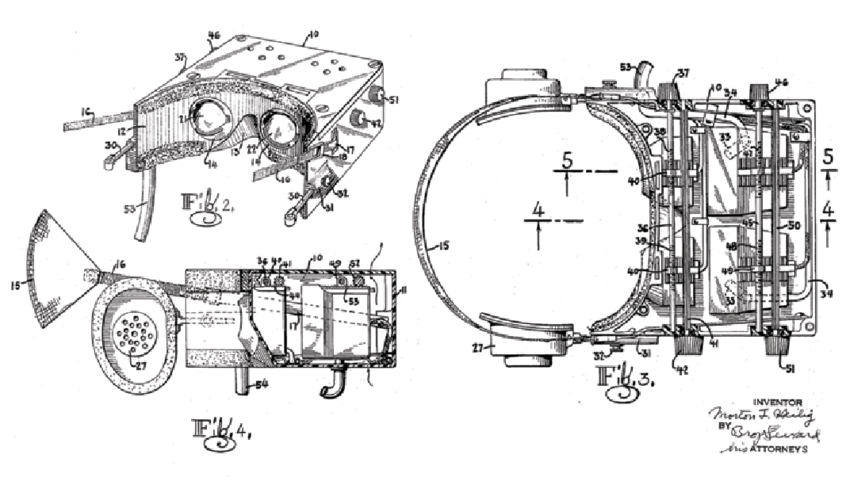
\includegraphics[width=\linewidth]{figures/telesphere-mask.png}
    \caption{Morton Heilig's patent for the Telesphere Mask~\cite{Heilig1994}, note the resemblance to contemporary headset design, such as the Meta Oculus Quest and the Apple Vision Pro.}
    \label{fig:telesphere}
\end{figure}

% what does it do?
%\cite{Wohlgenannt2020} % add othe citations mentioned in this paper
VR uses immersive technology to simulate interactive virtual environments where users feel physically present~\cite{Wohlgenannt2020, Bowman2007}.
This is done through the construction of a real or imagined environment, which blocks the real world from the user.
It also incorporates interaction methods such as controllers and motion tracking for the user to interact with the environment~\cite{Brooks1999, Barfield2000}.

% other VR tecnologies
% augmented reality (AR), augmented virtuality (AV), terms also refered to as mixed reality (MR) superimposes virtual agents over the real world in real-time (added digital information to physical reality)
% the term extended reality (XR) is a term used to refer to all the possible combinations of  real-and-virtual environments and human–machine interactions generated by computer technology and wearables
%  used as a umbrella term for their combined use

\begin{figure}
    \centering
    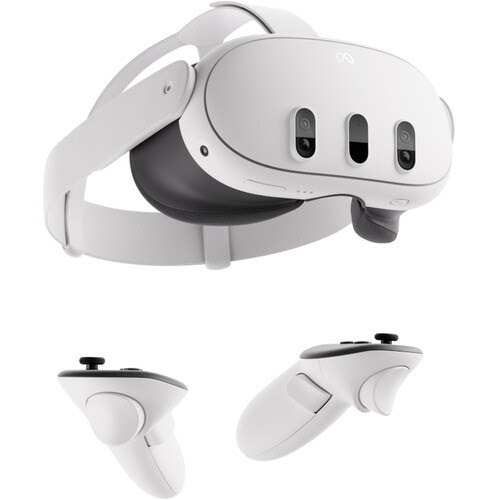
\includegraphics[width=0.6\linewidth]{figures/oculus-quest.jpg}
    \caption{An example of one of the latest iterations of VR technology, Meta's Oculus Quest 2. It can be considered as a extended reality (XR) headset as it can host VR environments while also incorporation augmented reality (AR) features.}
    \label{fig:oculus-quest-2}
\end{figure}

VR experience can be evaluated according to three key properties: presence, interactivity, and immersion~\cite{Walsh2002}.
% presense refers to the sense of physically being somewhere other where someone actually is
Presence refers to the sense of being physically somewhere.
Within a virtual environment, the presence of the user is simulated by capturing their senses, using visual, audio, and tactile simulations~\cite{Sanchez2005}.
% visual, ausio and tactil(haptics) realism is an important factor for presense in a virtual environment
% as well as virtual body representation and body engagement
The feeling of being present in virtual environments arises from the way that a user perceives and processes information from their surroundings, both in their conscious and subconscious environment~\cite{Barfield2000}.
% Some factors which contribute to how present a user feels in a virtual environment are: the virtual environment, communication medium, the individual user, any disturbances from the real world and, the task or tasks which the user performs.
% there are factors which contribute to presense
%   the computer and virtual environment
%   the communication medium
%   the individual
%   disturbances from the real-world environment
%   the task
The sense of presence that a user feels is difficult to quantify, as it can be measured in objective and subjective ways.
Subjective measurement comes from the level of realism in the virtual environment.
As VR technology improves, the level of realism VR headsets are able to display improves with it.
% Subjective measures of presense
%   realism is an essential part of presense in a virtual environment
%   as the technology used in contemporary VR headsets improve so does the realism and sense of presense within the environment
The objective measure of presence observes physical indicators in the user; these indicators include heart rate, dilation of the pupils, blink responses, and muscle tension.
% Objective measures of presense
%  physical indicators in a test subject (Heart rate, pupil dilation, blink responses, and possibly muscle tension)
Some more objective measurements include the extent to which physically reality is excluded from the virtual one, the number of the user's senses that are captured by the virtual reality, the extent of the field of view, the resolution and quality of the displays used, and how the user's body movements match up against their movements in the virtual world~\cite{Sanchez2005, Barfield2000}.
% objectively measurable 
%   inclusiveness - the extent to which reality is exculded
%   extensiveness - the range of sensory modalities
%   surrounding - the size of the feild of view
%   vivedness - the richness, resolution, and quality of the displays
%   matching - the extet to which proprioceptive feedback on body movementsin aligned with display information
% Immersion can be quantifiable judged through the assessment of the inclusively, extensiveness, display size and resolution of display technology~\cite{Barfield2000}.
% The aspect of inclusively refers to how much of the real world is the display able to block out from the vision, extensiveness refers to how many senses the technology encapsulates, such as taste, touch, sight, smell, and hearing.
% The display size judges how panoramic the display is and the resolution refers to the level of resolution or number of pixels on the display.
%   inclusive - the degree to which the stimuli from the real world are excluded from the user
%   extensive - the number of sensory modalities accommodated by the system
%   surroundings - how panoramic the displays are
%   vivid - the resolution of the displays
Interactions in the real world are naturally as good as they could possibly be according to both subjective and objective measurements of presence.
Human senses have specifically adapted for perceiving and interacting in the real world, and therefore it is difficult to simulate the same level of realism digitally.

VR Interactivity refers to how effectively a user can manipulate the virtual environment in real time~\cite{Steuer2000}.
In interactive systems, users have agency and control over various elements within the virtual environment, which allows them to make decisions, perform actions, and influence outcomes with their interactions.
This can range from simple actions like clicking buttons or navigating menus to more complex interactions such as manipulating objects, and altering parameters. 
The level of interactivity correlates with the user's sense of immersion and engagement, as it enables them to influence the environment and participate actively in the experience according to their preferences, goals, and intentions.
% interactivity refers to the extent to which a user can manipulate their environment in real time
Interactivity is a key factor as it affects the level of presence the user feels within the environment and directly influences the user's sense of presence. 
% interactivity can affect the presence the user feels within the environment (body engagement)
 
Immersion in VR is more complicated than presence and interactivity.
% It can be classified as subjective involvement which involves cognitive, emotional, sensory-motor, and spatial immersion.
Immersion can be described as subjective involvement, encompassing various dimensions of a user's experience~\cite{Nilsson2016}. 
However, there are many facets of immersion.
Cognitive immersion manifests when a user engages with the content, experiencing satisfaction and fulfilment upon solving complex problems. 
Emotional immersion occurs when a user become emotionally invested in narrative structures, experiencing highs and lows which come with a story. 
Kinesthetic immersion emerges when users receive immediate feedback on their physical actions, which enhances their sense of presence and agency within the virtual environment. 
% The term distal-attribute describes this phenomenon aptly, it is where an individual creates a mental representation of themselves to include the external and virtual worlds.
% For example, when a tool becomes and extension of an individual's body but it is not physically part of it.
% the phenomenon of individuals creating a mental representation of them selves to include in the external and virtual world.
% eg a tool becomes an extension of your body even though it is physically not
Spatial immersion is experienced as users navigate and perform intricate movements, feeling a sense of spatial presence and immersion within the simulated world. 
These dimensions collectively contribute to a rich and immersive user experience across various interactive platforms and media.
%  immersion can also be classifed as subjective involvement
%   cognitive immersion - users feel when they solve complex problems
%   emotional immersion - users feel when narrative structures unfold
%   sensory-motoric immersion - users feel when they receive feedback on movements
%   spatial immersion - users feel when they perform extensive maneuvers/
The sense of presence relates to the perception of the physical environment and is tightly coupled to how immersed the user feels.
Vice versa, the more immersed the user feels in the virtual environment, the easier it is for them to feel present.

While VR systems offer immersive experiences, they face some downsides, notably simulator sickness. 
This condition is caused by to frame rate drops.
Frame rate is the number of images a display such as a screen can cycle through per second.
The rapid succession of frames on the display is what causes the image on the screen to appear to have motion.
When the frame rate is high, the motion on the display appears smooth; low frame rate makes the motion of the image to appear choppy and unpleasant.
It is this choppy movement on the display which leads to a disconnect between user input and display output, which results in feelings of confusion, dizziness, and nausea for some users. 
% Simulator sickness can easily arise from a poorly designed or poorly performing system.
The level of susceptibility to simulator sickness varies between individuals, but has some dependence on a users experience with VR headsets as well as their natural tolerance to being in a VR environment.
Additionally, as the system's performance declines, the immersive element of the experience diminishes, which highlights the sensitivity of VR experiences to hardware performance. 
Users experience disconnect from the environment when any aspect of presence, interactivity, or immersion is compromised.
% A consequence of this disconnect is that a user may experience simulator sickness.
% Thus, the overall experience of a VR system heavily relies on consistent and high-performance hardware to maintain immersion and prevent adverse effects on users.
% the downsides
% simmulator sickness
% frame rate drop produces a disconnect between the user input and the display output causing a feeling of confusion, dizziness and nausea in some users
% the immsersiv element of the experience breaks down as the performance of the system drops
% the experience of a VR system is dependent on the hardware's performance and is incredible sensitive to drops in performance
\subsection{Visual Analytics}
\label{sec:visual-analytics}

Visual analytics is the practice of analysing datasets using visual representations of the data, these representations are the individual data points of the dataset mapped using a particular visualisation strategy \cite{Bikakis2018}. 
% Offer benefits such as visual perception, interactive exploration, improved understanding, informed steering, and intuitive interpretation~\cite{Li2016}.

Visualisations facilitate the emergence of patterns as they are explored by analysts, typically domain experts, enhancing accessibility, interpretation, and meaningful analysis of data~\cite{Lowe2020, Tukey1977} through interactive engagement with diverse tools.
These visualisations are made with goals in mind, which can be exploitative, confirmatory or for presentation~\cite{keim1997}.
Exploitative analysis involves undirected interaction with data which does not have a hypothesis attached to the exploration.
This type of analysis is done to construct a possible hypothesis relating to the data.
In contrast to confirmatory analysis has a more goal-oriented approach; the purpose of the exploration or examination of the data is to confirm or reject a hypothesis.
This is for the purpose of either confirming or rejecting the hypothesis.
The goal of presentation differs from the goal of a hypothesis where it is only concerned with the technique it uses to present the data to best represent the facts it wishes to communicate.
Human analysts are naturally equipped with sophisticated pattern recognition abilities~\cite{Hassan2011, Taylor2015, Sneiderman1996}, and applying these skills while interacting with data visualisations facilitates knowledge extraction~\cite{Caldarola2017, Yi2007, Becker1987, Glueck2014, Bikakis2018, Muhlbacher2014, Shneiderman2008}.
Large datasets within the Big Data field require analysts' cognitive abilities to make sense of the data, using perceptual grouping, image segmentation, and object recognition~\cite{Lowe2020}.
These skills allow elements such as clustering, outliers, patterns, and correlations between characteristics become apparent.
A visualisation can communicate the essence of a dataset quickly and effectively regardless of size~\cite{Fisher2012}.
The aim of visual analytics is to support the analysts' analytical reasoning and research with interactive visualisations of datasets~\cite{Tufte1983, Ali2016, Becker1987}.

For the users to explore the visualised datasets there must be some interactions they can perform to affect the representation~\cite{Yi2007} without interaction the representation would be a static image~\cite{Becker1987}.
Static images do offer value in visual analytics, but this value is limited once the dataset exceeds a certain size and the granularity of the data becomes too fine.
Interactions performed on the representation must produce an instantaneous change in the visualisation to maintain the user's attention.
There is a threshold of 10ms or less between interaction input and response to facilitate an uninterrupted dialog between the user and the data~\cite{Glueck2014, Li2016, MacKenzie1993, Muhlbacher2014}.
% \cite{Li2016, Zhao2017, MacKenzie1993, Becker1987}
% Visualisation system should retreive data fast enough so that the analist does not lose interest or lose a train of thought (focus and momentum)
% minimise the user's waiting time as much as possible

\subsubsection{Progressive visualisation}
As a user analyses a representation of the dataset, the visualisation should allow the user to steer the appearance of the visualisation through interaction and should also allow them to drill down into areas of interest within the data.
This is the process of progressive visualisation where initially a low fidelity representation is displayed and as it is explored, higher fidelity data is brought into the visualisation~\cite{Zhao2017, Ahrens2005, Rosenbaum2009, Li2016, Tufte1983}.
% To understand the context of the data it is more important to get a broad overview of the data than exact figures.
The user steers the visualisation's progression through the data and the visualisation changes as they explore the data~\cite{Zhao2017, Muhlbacher2014, Fisher2012}.
% Displaying  a  low  fidelity  representation  prior  to  loading  a high  fidelity  version  has  long  been  utilised  to  ensure  responsive  interaction  [4,14,19]. % check refs
% \cite{Zhao2017}
% progressive visualisation / progressive visual analytics
% produce intermediate results of the visualisation as the user explores the dataset
% the dataset can be sampled randomly to make these progressive visualisation or it can be arranged in a heirchical format.
The data stored at different levels of fidelity are pre-processed into a hierarchical order so that required data can be found easily~\cite{Glueck2014}.
% This method of storing data aligns with the exploration process the user undergoes when interacting with the visualisation~\cite{Rosenbaum2009}, the whole dataset is first shown to the user, and as they explore the model increases in resolution as they zoom in on areas of interest.
Pre-processing data used for visualisation can dramatically improve the user experience~\cite{Shneiderman2008}.
% Visualisation tools should give the user a high level overview initially and subsequently load more data as the user explores areas of interest~\cite{Li2016, Tufte1983}.
Some of the visualisation tools for interactions should include scaling, translation, rotation, filter, overview, and detail-on-demand~\cite{Zhao2017, Becker1987, Sneiderman1996, keim1997, Baracaglia2019, Ferrand2016}. 
%overview first, zoom and filter, then details on demand
% In three-dimensional datasets these interaction translation, rotation, croping, measurement and transparency \cite{Baracaglia2019, Ferrand2016}.

Scaling data correctly is important for lower-powered devices such as the VR headset and personal laptop computers, as they have comparatively fewer computational resources available.
The visualisation of points which translates to a size which is smaller than a single pixel on a screen is a waste of resources and should be minimised~\cite{Li2016, ertl1999}.

% \cite{Fisher2012}% information visualization, large amounts of quantitative data can be shown in a limited space
% graphical display extended to visualisations should
%   show the data
%   induce the viewer to think about the substance rather than about methodology, graphic design, the technology of graphic production, or something else
%   avoid distorting the message in the data
%   present a large amount of data in a small space
%   make large sets coherent
%   encourage the eye to compare different pieces of data
%   reveal the data at several levels of detail, from broad overview to fine structure
%   serve a reasonably clear purpose: description, exploration, tabulation, or decoration
%   be closely integrated with the statistical and verbal descriptions of the dataset

\subsubsection{Virtual reality in visual analytics}
Human eyes are naturally suited for three-dimensional space are more in accustomed to interacting with three-dimensional objects and VR simulates this interaction~\cite{Ferrand2018, Abidi2017}.
VR headsets provide an inexpensive and portable environment for multi-dimensional visualisations, which provides the ability to interact with the visualisation.
Three-dimensional data visualised in three-dimensional space grant a holistic view of the of the data~\cite{Ferrand2016, Farr2009}.
An effective visualisation bridges the gap between the data contained in datasets and the human ability to extract knowledge.
The stereoscopic environment produced by a VR headset such as the Oculus Quest 2 allows the user to see the data with a perception closer to a real-world environment, fostering user friendly interaction which resembles interaction in the real world.
% The VR headset also track the user's movement adding an extension of self into the VR environment for increased immersion
% While building the experimental system E0102-VR~\cite{Baracaglia2019} some insights were found involving the use of VR for viewing and interacting with multi-dimensional datasets.
% The depth perception provided by VR aids in understanding complex three-dimensional structures and provides means to quickly measure distances and angles in three dimensions.

% \cite{Ferrand2016}
% major challenges faced by astronomers is to digest the large amount of diverse data generated by modern instruments or simulations
% develop visualization tools that allow exploration of all their complexity and dimensions
% interested in displaying the 3D data in actual 3D space, to get a holistic view, in the expectation that this will generate a more correct perception, and help build an intuition, of the data.
% user friendliness - developing interfaces allowing for Natural User Interaction (NUI) in 3D is still an active field of research
% flat display of a desktop or mobile computer, the visualization is limited to 2D views: slices and projections, that have to be flipped through, or a fake 3D view, emulated with tricks like per- spective and shading.
% Stereoscopic 3D can be achieved using dual projectors, that present a slightly different image to each eye
% The 3D displays we are considering here bring something more: the tracking of the viewer (commonly using infrared cameras), which makes the experience distinctively different. First this enables motion parallax, which gives a much stronger depth cue, and second this allows direct interaction with what is being displayed. Depending on the hardware used, one can get the feeling of being fully immersed inside the data cube, as if it was a physical object that we can explore and manipulate.
% 3D displays for Virtual Reality come broadly into two categories: “fish tanks”, systems where the user is looking at a fixed screen or set of screens that define the boundaries of a virtual volumetric screen, and head-mounted displays (HMD), systems where the user is wearing a pair of screens attached directly in front of their eyes.
% serious applications in the medical and architectural fields, with also several experiments in the natural sciences: biology, geology, meteorology.
% ray casting: for each pixel to be rendered on the screen, a ray is cast along the current line of sight, and along this ray the data is retrieved at regularly spaced intervals. The values are accumulated along the line of sight using the standard radiative transfer approximation: the value at a point (understood here as a voxel) is interpreted as both an emissivity (added to the R, G, B channels) and an opacity (using the alpha channel to handle transparency)

% \cite{Ferrand2018}
% visualisation is important for exploring as well as the communication of data
% astronomy uses 3D data sets
% humans are more in tune to interact with 3D objects
% VR facilitates this interacting

% \cite{ertl1999}  hierarchical methods for visualisation of volume data
% basically introduces a hierarchical structure to the volume data so that it takes less time and memory to create a visualisation
% The standard model of this process comprises a pipeline of three stages. The filter stage is a preprocessing step converting the raw input data into visualization data which is usually reduced by operations like sampling, slicing, cropping, etc. The mapper stage performs a mapping of the abstract data fields into a visual representation consisting of geometric primitives like points, lines, surfaces or voxels and associated graphical attributes like color, transparency, texture, etc. The renderer, finally, uses this scene description to generate images by means of 3D graphics APIs such as OpenGL or OpenInventor, possibly exploiting 3D graphics hardware to achieve interactive frame rates.
% the user has to be given control over the threshold letting him choose between a fast visualization of a very crude approximation of the data and an almost perfect representation of the data which took perhaps minutes to compute. This requirement can only be met if not only one compressed version of the data, but a complete hierarchy of representations of the data set at different levels of resolution is available or can be generated on the fly.
% Direct volume rendering tries to convey a visual impression of the complete 3D data set by assigning different color and opacity values to different objects or value ranges within the volume. The resulting image is then computed by taking into account the so-defined emission and absorption effects as seen by an outside viewer. 
% Hierarchical approaches
%   

% \cite{keim1997}
% goals of visualisation
%   explorative analysis
%       start -> data without hypotheses about data
%       process -> interactive, undirected search for structures, trends, etc.
%       result -> visualisation of data, which provides hypotheses about data
%   confirmative analysis
%       start -> hypotheses about data
%       process -> goal orienatated examination of the hypotheses
%       result -> visualisation of data,which allows the confirmation or rejection of the hypotheses
%   presentation
%       start -> facts to be presented
%       process -> choice of presentation technique
%       result -> high quality visualisation of data presenting facts

% classifications of data visualisation techniques
%   geometric techniques -> scatterplots, landscapes, parallel coordinates
%       visualization of geometric transformations and projections of the data.
%   icon-based techniques -> stick figures, color icons, shape-coding
%       Visualization of the data values as features of icons.
%   pixel-orientated techniques -> spiral- , axes-techniques, recursive pattern techniques
%       each attribute value is represented by one colored pixel ( the value ranges of the attributes are mapped to a fixed colormap)
%       the attribute values for each attribute are presented in separate subwindows
%   hierarchical techniques -> treemap, dimensional stacking
%       Visualization of the data using a hierarchical partitioning into subspaces.
%   graph-based techniques -> basic graphs
%       Visualization of large graphs using techniques to convey the meaning of the graph clearly and quickly.

% Dynamic interaction techniques
% Dynamic generation of the visualizations or interaction with the visualization for a more effective exploration of the data
%   data-to-visualisation mapping
%   projections
%   filtering (selection, querying)
%   linking, brushing
%   zooming
%   detail on demand

% data pre-processing techniques
%   Dimension reduction techniques
%       principal component analysis -> Determines a minimal set of principal components (linear combinations of the original dimensions) which explain the main variations of the data.
%       factor analysis -> Determines a set of unobservable common factors which explain the main variations of the data. The original dimensions are linear combinations of the common factors.
%       Multidimensional Scaling -> Uses the similarity (or dissimilarity) matrix of the data as defining coordinate axes in multidimensional space. The Euclidean distance in that space is a measure of the similarity of the data items
%       fatsmap -> Fastmap also operates on a given similarity matrix and iteratively reduces the number of dimensions while preserving the distances as much as possible.
%   Subsetting techniques
%       (Set of Data Items -> Subset of Data Items)
%       Sampling (determines a representative subset of the database
%       Querying (determines a certain, usually a-priori fixed subset of the database)
%   Segmentation techniques
%       (Set of Data Items -> Set of (Set of Data Items)
%       Segmentation based upon attribute values or attribute ranges
%   Aggregation Techniques
%       (Set of Data Items -> Set of Aggregate Values
%       Aggregation (sum, count, min, max, ...) based upon attribute values, opological properties, etc.
%       Visualizations of Aggregations: Histograms, Pie Charts, Bar Charts, Line Graphs, etc
\subsection{Data Visualisation}
\label{sec:data-visualisation}
This section will summaries the different techniques and strategies used to create visualisations of astronomy data cubes or any volumetric data. 
% explain volumetric data
Volumetric datasets can be thought of as data cubes as they have data along the \textit{x}-,\textit{y}- and \textit{z}-axes. 
They are commonplace in fields such as astronomy, medicine, oceanography, molecular modelling, and engineering.
Data cubes can be described as a set of samples \textit{(x, y, z, v)}, where the value of \textit{v} is some property of data at the three-dimensional coordinates \textit{(x, y, z)} \cite{Kaufman2000}.
A point within a data cube is a three-dimensional pixel and is referred to as a voxel or volume pixel~\cite{Kaufman1996}.
In astronomy datasets \textit{x} and \textit{y} are used for spatial information where the third axis, \textit{z}, is usually a red-shift value, not distance.
The steps through the \textit{z}-axis are refereed to as channels and the number of channels on the \textit{z}-axis depends on the velocity resolution and bandwidth of the receiver~\cite{Taylor2015}.
% the high dynamic range makes assigning colours difficult
% a representation of a point in a three-dimensional dataset is called a voxel or volume pixel which is essentially a three-dimensional pixel and has an x, y, and z coordinate
% These datasets are essentially represented as a three-dimensional scatter plot.
The data is a representation of a measurable property of astrophysical phenomenon, and can be represented as binary values or values within a range.
% the data can be binary, represented as zeros and ones or be multivalued and be a representation of some measurable property
% start by stating why visualisation is important
% what does visualisation do for astronomy data

% -------------
Data visualisation is the presentation of data as a static or interactive image~\cite{Bikakis2018}.
Visualisation is imperative to making sense of abstract datasets such as those prevalent in radio astronomy research ~\cite{Glueck2014, Yang2017},
and is important for the exploration of data and the communication of findings~\cite{Ferrand2018}.
Visualisations allow enormous amounts of quantitative data to be shown in a limited space, while also maintaining the message contained within the dataset~\cite{Fisher2012}.
% Allows the user to see the data without concerning themselves with the methodology or the technology of the graphical production.
% How astronomers use their skills in visual analytic to extract knowledge from these visualisation is inspected further in Section~\ref{visual-analytics}.
Data visualisation has some distinct objectives~\cite{Norris1994, McReynolds2005, Hassan2011}: 
\begin{itemize}
    \item Allow the user to explore the data and obtain a deeper understanding~\cite{Bikakis2018}.
    \item Expose features within the dataset which would otherwise have remained hidden.
    \item Obtain quantitative results from the data, and communicate the results to others.
\end{itemize}

\begin{figure*}
    \centering
    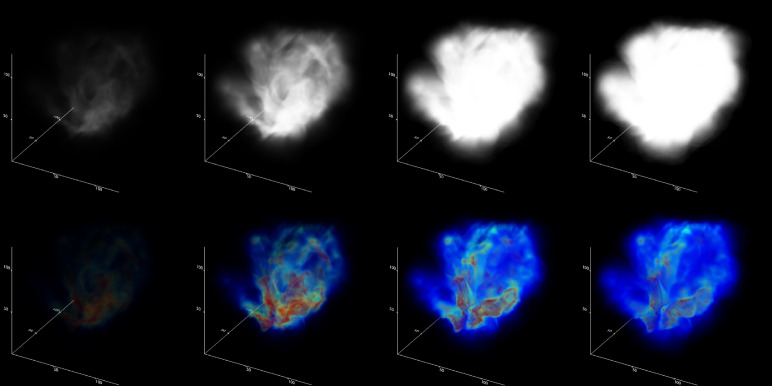
\includegraphics[width=1\linewidth]{figures/volume.jpg}
    \caption{An astronomy dataset visualisation generated by Frelled~\cite{Taylor2015} depicting how the addition of colour and opacity applied to the voxels effectively exposes hidden structures within the dataset. It shows how various ranges of opacity affect the visualisation but also how colour adds to its readability.}
    \label{fig:volume}
\end{figure*}

% Visualisation plays an integral role in allowing the visualisation to be interactively steered,
% the importance of visualisation and interaction for visual analysis is discussed further in Section \ref{visual-analytics}.

% visualisation challenges
There are certain characteristics present in the data which make visualisation difficult~\cite{Hassan2011}.
The datasets produced by astronomy data gathering instruments produce massive amounts of data, giga-bytes to peta-bytes, large enough to fill the memory of multiple conventional desktop computers.
This makes the datasets difficult to manage and process for visualisation.
There is no dominant file type used to represent astronomy data, which makes the development of a generic visualisation tool difficult.
Conventionally FITS files~\cite{wells1979} have been used to represent data cubes.
The cubes are divided up into slices along the \textit{z}-axis. 
Each of the these slices can be visualised as an image consisting of pixels with an \textit{x} and \textit{y} coordinate.
A user can move through slices of a data cube sequentially and can be played through like frames in a movie.
A major downside of visualising the data in this manner is that it does not let the user get an impression of how the dataset looks as a whole.
Therefore, limiting how quickly and effectively a user can construct a mental model and begin extracting insight~\cite{Norris1994}.
% bottleneck between human and machine where it is difficult for the user to construct model of the information in their mind in a way in which knowledge can be extracted
That data also has a high dynamic range and a low signal-to-noise ratio, which makes distinguishing genuine sources between large portions of noise difficult for astronomers.

\subsubsection{Visualisation Techniques}
There are different visualisation techniques which can be used to produce a representation of the dataset.
However, the nature of the data dictates the appropriate visualisation method to be used~\cite{Hassan2011}.
The common techniques used for generating comprehensive visualisations of a volume dataset are points, splats, iso-surfaces, and volume rendering.
% In the absence of a comprehensive visualisation, astronomers rely on techniques such as data-slicing or projected moment maps to aid research.
%\cite{Norris1994}% the most common techniques for representing astronomy volume data

\begin{figure}[h]
    \centering
    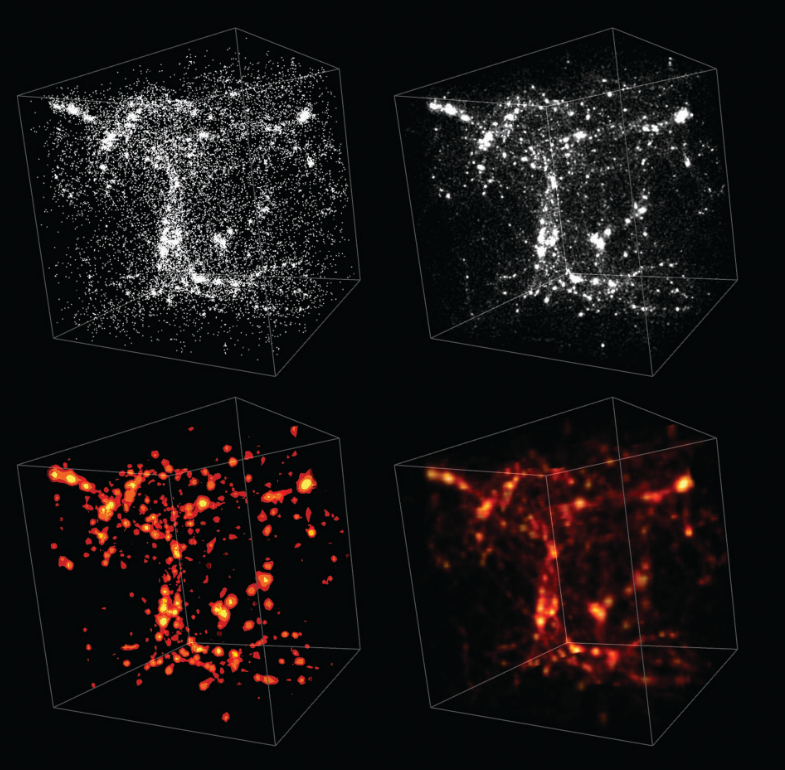
\includegraphics[width=\linewidth]{figures/visualisation.png}
    \caption{Four visualisations of an astronomy dataset using the common visualisation techniques~\cite{Hassan2011}, clearly depicting how the different visualisation techniques affect the presentation of the data. Point (top-left), splats (top-right), iso-surface (bottom-left), and volume rendering (bottom-right).}
    \label{fig:visualisation}
\end{figure}

\paragraph{Points}
% points
%   approach is limited by the available resolution (or pixeldensity) of the display
Each point in a dataset represented as a fixed-width pixel to a picture plane as if it were a three-dimensional scatter-plot.
While it is the most straightforward technique for representing data, this approach is limited by the available resolution or pixel density of a display.
This is not a suitable method for visualising astronomical data.
Simply plotting the data as a three-dimensional scatter plot makes it difficult to derive meaning from the data visualisation.
For example, the top left quadrant of Figure \ref{fig:visualisation} when compared to the bottom right quadrant is much less semantically comprehensible.

\paragraph{Splats}
This visualisation technique uses small two-dimensional textures to represent data points, and uses a method known as ``bill-boarding"~\cite{Taylor2015}, to ensure the textures always point towards the camera regardless of the scene's orientation.
When many splats are combined, this produces an effect that is much like volume rendering, but without the computational overhead of ray-tracing.

\paragraph{Iso-surface}
Polygon-based rendering, also referred to as surface rendering, is used to visualise volume data using polygons.
% three-dimensional equivalent of contouring
The majority of three-dimensional models use this method to represent their forms.
Surfaces or polygons must be extracted from volume data before it can be visualised.
Part of the visualisation process involves determining where the boundaries of the objects are and defining a skin for each region.
There are various methods for calculating these boundaries, such as: marching cubes, marching tetrahedra, multi-resolution iso-surface extraction, and surface wave propagation.
%   methods for calculating an isosurface from a data-set (check source for citations of the different methods)
Iso-surface rendering is commonly used to search for correlations between different scalar values, but is not used as a visualisation method because the visualisation is not comprehensive enough for knowledge extraction.
%   usually used to to searcg for correlation between different scalar values but are not as good at giving the overall picture of the dataset
% transparency is difficult
% boundaries could leave out interesting structures

\paragraph{Volume Rendering}
This technique renders each data point as three-dimensional pixels, also referred to as voxels. 
Voxels are arranged on the x-, y- and, z-axes to construct a three-dimensional image.
To make these structures more comprehensible, a colour transfer function is used to assign an opacity and colour to each voxel.
% volume rendering
%   provides a global view of the data-set
%   renders the external surfaces as well as the internal three-dimensional structure
%   ability to display weak or fuzzy surfaces
%   uses colour transfer function to assign an opacity and colour to the voxels
% uses ray-tracing or ray-marching shaders which can be computationally expensive
Volume rendering uses ray-tracing or ray-marching shaders to render the visualisation.
These types of shaders use significantly more computing resources compared to the traditional shading model~\cite{Wittenbrink2000}.
There are several optimisations and acceleration techniques that can tailor the shader to data being visualised.
% various algorithms for volume rendering
% back-to-front
% front-to-back
% shearing
% ray-casting
%   casts a ray from each pixel on the screen into the volume data along the viewing vector until it accumulates an opaque value
% ray-tracing
%   ray tracing is referred to as the process where reflected and transmitted rays are traced
However, it is a favoured method for representing volume data as it produces a complete view of the external surface as well as the internal three-dimensional structures within the dataset.

\subsubsection{Two-dimensional versus Three-dimensional Visualisations}
Three-dimensional visualisation techniques are better-suited for representing volume datasets, compared to two-dimensional visualisation techniques.
% why 3D is better suited for astronomy data than 2D visualisations

Some intuitive understanding of the data is missed when the data is examined using two-dimensional approaches~\cite{Kent2013}.
These approaches examine pieces of the data, such as individual slices from the dataset, or are played through sequentially like a movie.
This method of examination does not allow the user to observe the dataset as a whole.
% an intuitive understanding is missing when only examining data visualised with 2D approaches
% approaches where the iundividual channels or slices of a data cube are examined seperately 
Three-dimensional visualisations highlight hidden features within the data that would otherwise have remained hidden~\cite{Ferrand2016}.
% 3D vis techniques highight hidden features within the data that would have otherwise gone unnoticed
Comprehensive visualisations are important for communicating results quantitatively.
Therefore, visualisation which represent the data in a more comprehensive way is preferred.
% visualisation is important for communicating results quantitavely

%%%%%%%%%%%%%%%%%%%%%%%%%%%%%%%%%%%%%%%%%%%%%%%%%%%%

% challenges for petascale astronomy era
% \cite{Hassan2011}
% support of quantitative visualisation
% effective handling of large data-sets
% discovery in low signal-to-noise data
% better human-computer interaction and ubiquitous computing
% better workflow integrtion
% encouragement of adoption of 3D scientific visualisation techniques

%\cite{Hassan2011} % allow analysis to see the underlying large-scale structures hidden in the volumetric data set 
% by colour coding the points or applying a surface function to the data

% \cite{Sneiderman1996}
% mantra: overview first, zoom and filter, then details on demand
% seven data types (one-, two-, three-dimensional data, temporal and multi-dimensional data, and tree and network data)
% seven tasks (overview, Zoom, filter, details-on-demand, relate, history, and extracts).
% Exploring information collections becomes
% increasingly difficult as the volume grows.
% but the opportunity for dynamic displays takes user interface designers well beyond current wisdom. -> VR section in visual analytics
% Overall, the bandwidth of information presentation is potentially higher in the visual domain than for media reaching any of the other senses -> visual analytics section
% Users can scan, recognize, and recall images rapidly, and can detect changes in size, color, shape, movement, or texture

% \cite{Shneiderman2008}
% the purpose of visualising is insight not pictures
% the heart of information visualization is the well-designed user control panel and interaction techniques that enable users to generate task-related comprehensible coordinated windows
% The successful tools support a process of information-seeking that leads to important insights
% The successful visualization tools apply carefully designed data structures that run in the high speed store (RAM), so that even users of laptops with a few gigabytes of RAM can interactively explore million record databases.
% millions of records can translate to millions of data points within a volumetric dataset
% Billion record databases will require compression strategies or innovative hierarchical data management
% Precomputing of anticipated data needs can dramatically improve the user experience.

% \cite{Kaufman1996}
%  Volume visualization is a method of extracting information from volumetric datasets through interactive graphics and imaging, and is concerned with the representation, manipulation, and rendering of these datasets
% Volume data are 3D entities that may have information inside them, may not consist of surfaces and edges, or may be too voluminous to be represented geometrically.
% The primary sources of volume data are three: sampled data of real objects or phenomena, computed data produced by a computer simulation, and modeled data generated from a geometric model
% Examples of applications generating sampled data are medical imaging (e.g., CT, MRI), biology (e.g., confocal microscopy), geoscience (e.g., seismic measurements), industry (e.g., nondestructive inspection), and chemistry (e.g., electron density maps)
% volume cell (voxel for short), with each voxel being a rectangular cuboid havingsix faces, twelve edges, and eight corners.

% \cite{Kaufman1993}
% volume visualisation is a method for extracting meaningful information from volumetric datasets through the use of inteactive graphics and imaging. \cite{Rosenblum1994}
% provide mechanisims for peering inside volumetric datasets
% 3D voxel is the counterpart to the 2D pixel

% \cite{Rosenblum1994}
% that is, the basic ide a of using c omputer-generated pictures to gain information and understanding from data (geometry) and relationships (topology)


\subsection{Rendering}
\label{sec:rendering-strategy}
% strategies for rendering large amounts of data without storing it on the client computer
The visualisation of large amounts of data becomes problematic when processing the data consumes all of the computational resources of a non-specialised system. 
This is because the resource requirements for processing increase with the size of the data-sets~\cite{Shneiderman2008}. 
Visualisations of large data cubes can still be produced by systems with specialised hardware, but these systems are often limited by their connection to a single geographical location and restricts the number of users able to access the system at a given point in time.
% yanG2017 every line has a source in this bloody paper - refer for more sources
% visualisation is essential to make sense of the data
Visualisation of data is essential to acquire an understanding of it~\cite{Yang2017}. 
Additionally, making the visualisation interactive increases its effectiveness. 
The addition of interaction increases computational overhead as the dataset being visualised must be rendered for each frame displayed.
Changes in the visualisation's appearance resulting from interactions should be perceived as instantaneous. 
Developing a system for producing interactive visualisations of gigantic datasets in real-time is a challenge because hardware will always be pushed to its limits. 
Waiting for hardware technology to catch up with the size of the datasets is futile, as the datasets also increase in size at a steady rate over time.
The increasing size of the datasets can be attributed to many things, but specifically in astronomy it stems from data-capturing instruments becoming more sensitive and more accurate.
To solve this problem would require a system which can scale consistent performance with the ever-increasing datasets without relying on the brute-force strategy for producing visualisations~\cite{Ali2016}.
In the brute force strategy, every single data point within the dataset is visualised regardless of the size of the dataset.

While visualising the entire dataset produces a highly accurate depiction of the data, the amount of time it takes to produce the visualisation is directly linked to the computational power of the hardware.
It could potentially take a long period of time to produce the visualisation if the visualisation is produced on lower-powered hardware~\cite{Fisher2012}.
The length of time can be affected by hardware issues such as system bandwidth, which depends on factors such as the graphical computations, the speed of the display hardware, and the speed at which information can be passed between components~\cite{Becker1987}.
All of the factors present bottlenecks where system performance is potentially stunted.

The rendering speed of the visualisation is crucial to user experience~\cite{MacKenzie1993}, especially in the context of VR, where if the time between updates takes too long it could cause simulator sickness in the user, making the system unusable from the user's perspective. % look for simulator sickness source
For devices with lower-powered hardware to be able to process and visualise the data without negatively affecting system performance the dataset must be reduced in size to reduce the amount of time required to produce a visualisation.
Either through breaking the dataset up into smaller pieces~\cite{Masiane2019, Li2016} or using some sort of data reduction technique to reduce the overall resolution of the dataset through downsampling techniques such as filtering, clustering and sampling~\cite{Masiane2019, Glueck2014}. 

There are problems with both of these approaches.
Dividing the data cube into subsections has the potential to affect the integrity of the data and obscure the context of a section within the larger dataset \cite{Abidi2017}. 
Downsampled data does attempt to preserve as much detail as possible \cite{Dumitrescu2019}, although the integrity of the data cube is affected and some data can be lost.
If the time reduction provided by downsampling the data obscures potential insights, the visualisation becomes useless.
Both of these techniques reduce the accuracy of the visualisation.

The accuracy with which the visualisation is depicted in is incredibly important to the analysis of the data, as discussed further in Section \ref{sec:visual-analytics}.
It is advantageous to give the user a high-level overview of the data at the start if their workflow\cite{Li2016, Lowe2020, Zhao2017}.
This overview can be a downsampled version of the data, which would reduce the processing time because there is less data to be visualised overall\cite{Masiane2019}.
The user must be able to dig deeper into certain areas of interest in order to explore the dataset and uncover insights.
In the architecture of the astronomy visualisation system i-Davie \cite{Marchetti2020}, the user is initially presented with a downsampled version of a data cube and can then explore smaller sections at higher levels of resolution.
i-Davie was made for the exploration of data cubes on a VR device, but the majority of the computation is performed on a co-located computer, typically with mid-range computational power and a GPU.
The i-Davie system workflow is as follows, the user explores the initial data cube and finds an area of interest they would like to explore further.
The user selects that area and crops the section.
i-Davie fetches the higher-resolution version of the selected portion of the data cube.
The user sees these intermediate results at the early stage of the data processing, which allows them to do further exploration based on current knowledge.
This method of progressive visualisation facilitates the exploration of large data cubes.
It allows for speedy access to a visualisation and minimises processing time~\cite{Zhao2017} while also maintaining the accuracy and integrity of the data \cite{Masiane2019}.
% The user sees partial results at the early stage of the data processing and allows them to do further exploration based on a current view to extract knowledge from the data \cite{Zhao2017}.
This method provides required data on demand but does not overwhelm the user with too much information at once.
Even if it is a subsection of the larger data cube the context of the piece of data is understood.
The user understands how that particular section relates to the whole data cube.
This rendering strategy supports the user workflow~\cite{Hassan2011},
initially presenting the user with the full-resolution visualisation does not have a significant improvement to knowledge extraction as, the level of detail visible on the display is limited by the display's resolution. 
The visualisation wastes computational resources by attempting to render points which corresponds to an area smaller than a pixel on the chosen display hardware.
% --------------------------------------------------------------------% what is remote rendering
\subsubsection{Remote Rendering}
The remote rendering strategy is an approach to rendering which offloads computational overhead from lower-powered hardware, such as a laptop or personal computer, to higher-powered hardware, such as a dedicated server.
It makes use of the client-server model;
the server component stores the large data-sets and performs the computationally expensive processes,
whereas the client provides input as requests to the server and displays the output of these requests to the user.
This makes it possible to produce visualisations of datasets which are larger than the client's resources can accommodate~\cite{Hassan2011}.
For remote rendering to function as intended, the client must be able to access any portion of the dataset, and the server and client systems must coordinate with each other to render and display the visualisations in real time~\cite{Glueck2014}.
There are also bottlenecks present in this approach that must be considered.
% network is the biggest bottleneck - want to minimise the overall amount of data sent from server to client as well as the client to the server
The largest bottleneck is the amount of data than can be sent through a network channel in a period of time~\cite{Abidi2017}.
To mitigate the bottleneck the amount of data transferred between the server and client systems needs to be minimised.
% compression is the most common method for counteracting this bottleneck
Compression is the most common method for reducing the bottleneck.
However, compression and decompression consumes CPU on both the client and the server systems and adds time to the rendering process.
It also presents the added chance of losing data during the compression-decompression process.
The system would use lossy or lossless compression, depending on the type of data and how important the integrity of the data is to the functionality of the system.

There are two rendering strategies present in remote rendering; server-side and client side rendering, both of which are prevalent in web application development.
Systems choosing an appropriate approach for their system architecture must consider which strategy would compliment the functionality of the system ~\cite{Iskandar2020}.
% comparison between client-side and server-side rendering in web development
% software architecture
%   choose the right architecture pattern to use to maximise/optimise the utilisation in the given context the application will be used
%   different architectural patterns
%       layered, client-server, master-slave, pipe-filter, broker, peer-to-peer, event-bus, model-view-controller(layered), blackboard, interpreter
% server-side - better search engine optimisation
% client side - better user experience

\paragraph{Client-side Rendering}
% request, download bundle, extract bundle being the web application
In client-side rendering, data is downloaded from a server and then rendered in the client browser.
More specifically, in a web application a request is made to a server, a bundle of data is downloaded.
Once the bundle reaches the web application it extracts the data from the bundle and uses the data in application.
These types of applications use API calls or WebSocket connections to request a from servers.
The process of rendering of volumetric data is the same, data is stored on the server, the data is bundled and sent to the client, the data is extracted and then rendered to produce a visualisation on the client system.
% reduces latency but affects/reduces accuracy
This reduces processing time by rendering the data on the client system.
The compression and decompression of the data during the transfer process can affect its accuracy.
The integrity of the data could also be affected by the downsampling process it went through on the server..
The amount of data that can be rendered is limited to the computational power of the client system while the client system performs other tasks besides those related to the rendering of the data visualisation~\cite{Becker1987}.
In a comparison between client-side and server-side rendering, client-side produces a better user experience~\cite{Iskandar2020}, as the interactions performed on the client are perceived as instantaneous.

\begin{figure*}
    \centering
    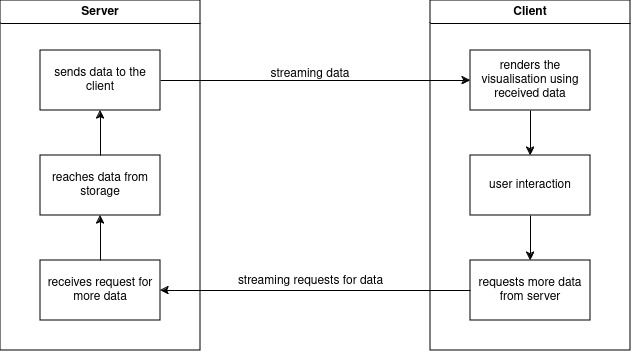
\includegraphics[width=0.6\linewidth]{figures/client-side-rendering.jpg}
    \caption{An example of the process of client-side rendering where data is sent from the server to the client to be rendered. The user interacts with the data on the client and only requests more data from the server when it is required.}
    \label{fig:client-rendering}
\end{figure*}

\paragraph{Server-side Rendering}
% Server side rendering is were static or semi-static web-pages are hosted on a server, and when the user opens a websites these pages are sent from the server.
Server-side rendering involves storing the data on the server and also rendering the data into a visualisation on the server.
Frames of this visualisation are sent to be displayed on the client web application.
% server handles requests from the client, performas actions, and returns a response
The client system has no part in the rendering process, it just displays the frames it receives from the server. 
The user can manipulate the visualisation by forwarding input capture by the client application to the server, following the classic request-response model for web applications.
% In remote visualization (or remote computation) heavy graphics tasks are delegated to a high-end graphics server that actually performs the 3-D rendering and generates a 2-D frame that can be visualized on a remote device (possibly characterized by limited hardware resources). 
The server renders the three-dimensional visualisation of the data but streams two-dimensional images to the client.
% Server-side rendering is implemented when there are computationally expensive graphics tasks that need to be performed.
% These tasks are delegated to the server which has enough computational resources to perform them, whereas the client system does not have the hardware resources to produce the visualisation~\cite{Becker1987}.
% increases accuracy but increases latency 
This strategy increases the accuracy as the integrity of the data is unaffected as it is not processed or transferred, however, it does increase processing time.
The main point where this processing time becomes apparent is when the user performs interactions with a visualisation on the client system.
The user must wait for the interaction to be forwarded to the server, then the visualisation must be re-rendered, and finally the updated frames are streamed to the client.
The time in which these tasks are done increases if the frames are also compressed for transfer over a network, and subsequently decompressed on the client.
The speed of the network the frames are streamed on also affects the processing time of the feedback to the user on the client system.
The slower the network, the more time the user has to spend waiting for feedback.
The server could also have a delayed response because it is performing other tasks, and handling many clients' requests~\cite{Becker1987}.

\begin{figure*}
    \centering
    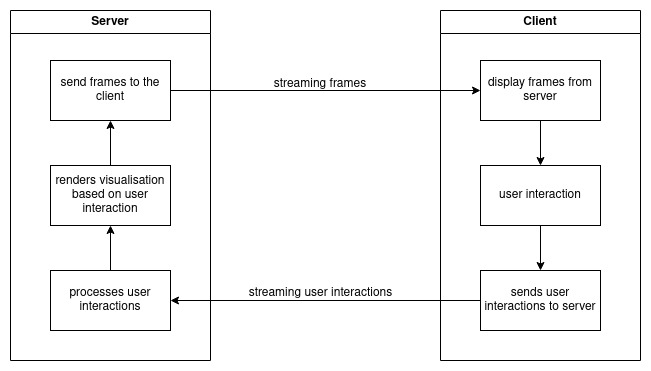
\includegraphics[width=0.6\linewidth]{figures/server-side-rendering.jpg}
    \caption{An example of the server-side rendering process, where the rendering of the data is done on the server and the frames are streamed to the client. The user interacts with the visualisation on the client but the interactions are sent to the server. The rendering is updated based on the user interactions and the frames are once again streamed to the client.}
    \label{fig:server-rendering}
\end{figure*}
\subsection{Current Visualisation Systems}
\label{sec:current-systems}
Extremely large datasets are commonplace within radio astronomy research. 
As this research progresses, the datasets are predicted to balloon in size even more at ever faster rates.
Advances in astronomical technology, such as larger detectors, increases in bandwidth, and astrophysical simulations, drive the need for visualisation solutions.
Specialised systems have been developed to cater to this aspect of astronomy data, as well as to astronomy researchers. 
While not all of these systems attempt to apply a generalist approach to volumetric data visualisation, important points can be taken from the systems reviewed.
The system architectures and strategies employed to handle the enormous amount of data produced by modern radio astronomy data-capturing instruments emphasise points that can be applied to various systems, as there are some shared goals.
Sources~\cite{Ferrand2016, Hassan2011, Naiman2016, Kent2013, Shneiderman2008} highlight a need for a generic standalone, cross-platform application capable of processing and visualising large amounts of volumetric data. 
These visualisations, used in addition to traditional statistical visualisations, have complementary effects on knowledge extraction by communicating information clearly and effectively~\cite{Caldarola2017, Goodman2012, Naiman2016, Rosenblum1994} especially as the variety of data grows and becomes more complex.
% want for a cross platform appication capable of processing and visualising various types of astronomy data formats, especially as those format grow evermore complex

\subsubsection{Big Data Visualisation Systems}
While not specifically geared towards astronomy data visualisation, these systems face similar issues handling large amounts of scientific data, and reviewing some of these systems could add valuable insight which can be applied to the development of radio astronomy visualisation systems.

% The big data era has made many very large datasets available, they are dynamic and characterised by high variety and volitility where new data is constantly being added
\textit{Big data} as a term can be defined as ``datasets whose size is beyond the ability of software tools to capture, store, manage, and process''~\cite{manyika2011, Sneiderman1996} or ``data which exceeds the capabilities of commonly used hardware environments and software tools to capture, manage, and process it within a reasonable amount of time''~\cite{merv2011}.
These datasets have characteristics relating to the three V's of \textit{big data}: volume, velocity, and variety.
As volume increases, problems involving processing, storing, and extracting knowledge arise.
When variety increases it complicates the storage and analysis of the data because of the different structures of data being stored.
Velocity relates to the speed at which data is generated, this has the potential to compound the issues of storing and processing a high volume of data~\cite{Caldarola2017}.
This is because processing data takes time and if data is not process fast enough it creates a backlog when new data is inbound.

There are various software packages and platforms to assist the user in making sense out of massive amount of information, each tailored to a specific use case.
For big data visualisation and analytics, great consideration must be put into the method of visualisation because the structure of the data affects the resulting visualisation.
Generally the tools value flexibility and user convenience.
By making these tools available on multiple platforms for ease of access and by having them be programming language agnostic, allowing the user to cutomise their workspace.
% There is a wide range of data plotting software that can be used to tailor a solution according to the data that needs to be analysed.
% RNeo4J, Statnet, Tableau, infogram, Tulip

A general solution to visualisation and analytics is complicated because it is impossible to account for all methods of visualisation and for the variety of data.
But most are aimed towards business analytics.
Some examples of data visualisation software for specific data types are:
\begin{itemize}
  \item Timeline - specialised to create interactive timelines from a spreadsheet
  \item Commetrix and Cuttlefish - used for dynamic network visualisation and analysis
  \item Cytoscape - used for visualising molecular interaction networks and biological pathways, originally designed for biological research but is now also used for complex network visualisation and network analysis
\end{itemize}

Current systems used for exploration and visualisation cannot handle the size of many contemporary datasets and restrict themselves to analysing only comparatively small data-sets.
This is mainly due to them using a brute force method of visualising the entire dataset regardless of how it will appear on a display~\cite{Bikakis2018}.
% offline - use a single local machine to generate the visualisations

The free-to-use game engine Unity~\cite{Marchetti2020, Ferrand2016, Ferrand2018} and the open source three-dimensional modelling and animation software Blender~\cite{Taylor2015, Taylor2016, Kent2013, Naiman2016} have been used for fast prototyping of various astronomy visualisation systems.
Blender is favoured for three-dimensional rendering capabilities and it three-dimensional space manipulation tools,
particularly useful for generating animations and graphics with astronomy data.

\paragraph{ParaView}
ParaView~\cite{Ahrens2005}, is an example of a tool created for scientists to visualise and analyse extremely large data-sets,
while emphasising the workflows of the domain experts.
It highlights speed and performance as key aspects of the software's functionality.
Its rendering strategy involves executing programs in parallel on either shared or distributed memory resources.
% supports hardware accelerated parallel rendering
% acheives interactive rendering performance via level-of-detail techniques
It can achieve high frame rates suitable for interaction by utilising level-of-detail techniques.
These level-of-detail techniques, also known as progressive visualisation, involve storing the dataset at many different resolution levels, which are also know as mipmaps.
They reduce the amount of data that has to be rendered, which also impacts the quality of the visualisation.
The dataset being visualisation must find a balance between the resolution of the data and the performance of the system
%  advantage of progressivly refining a coarse model of the data
% But leveraging the advantages of refining a coarse model of data and refining parts as the user works through the data.
\begin{figure*}
    \centering
    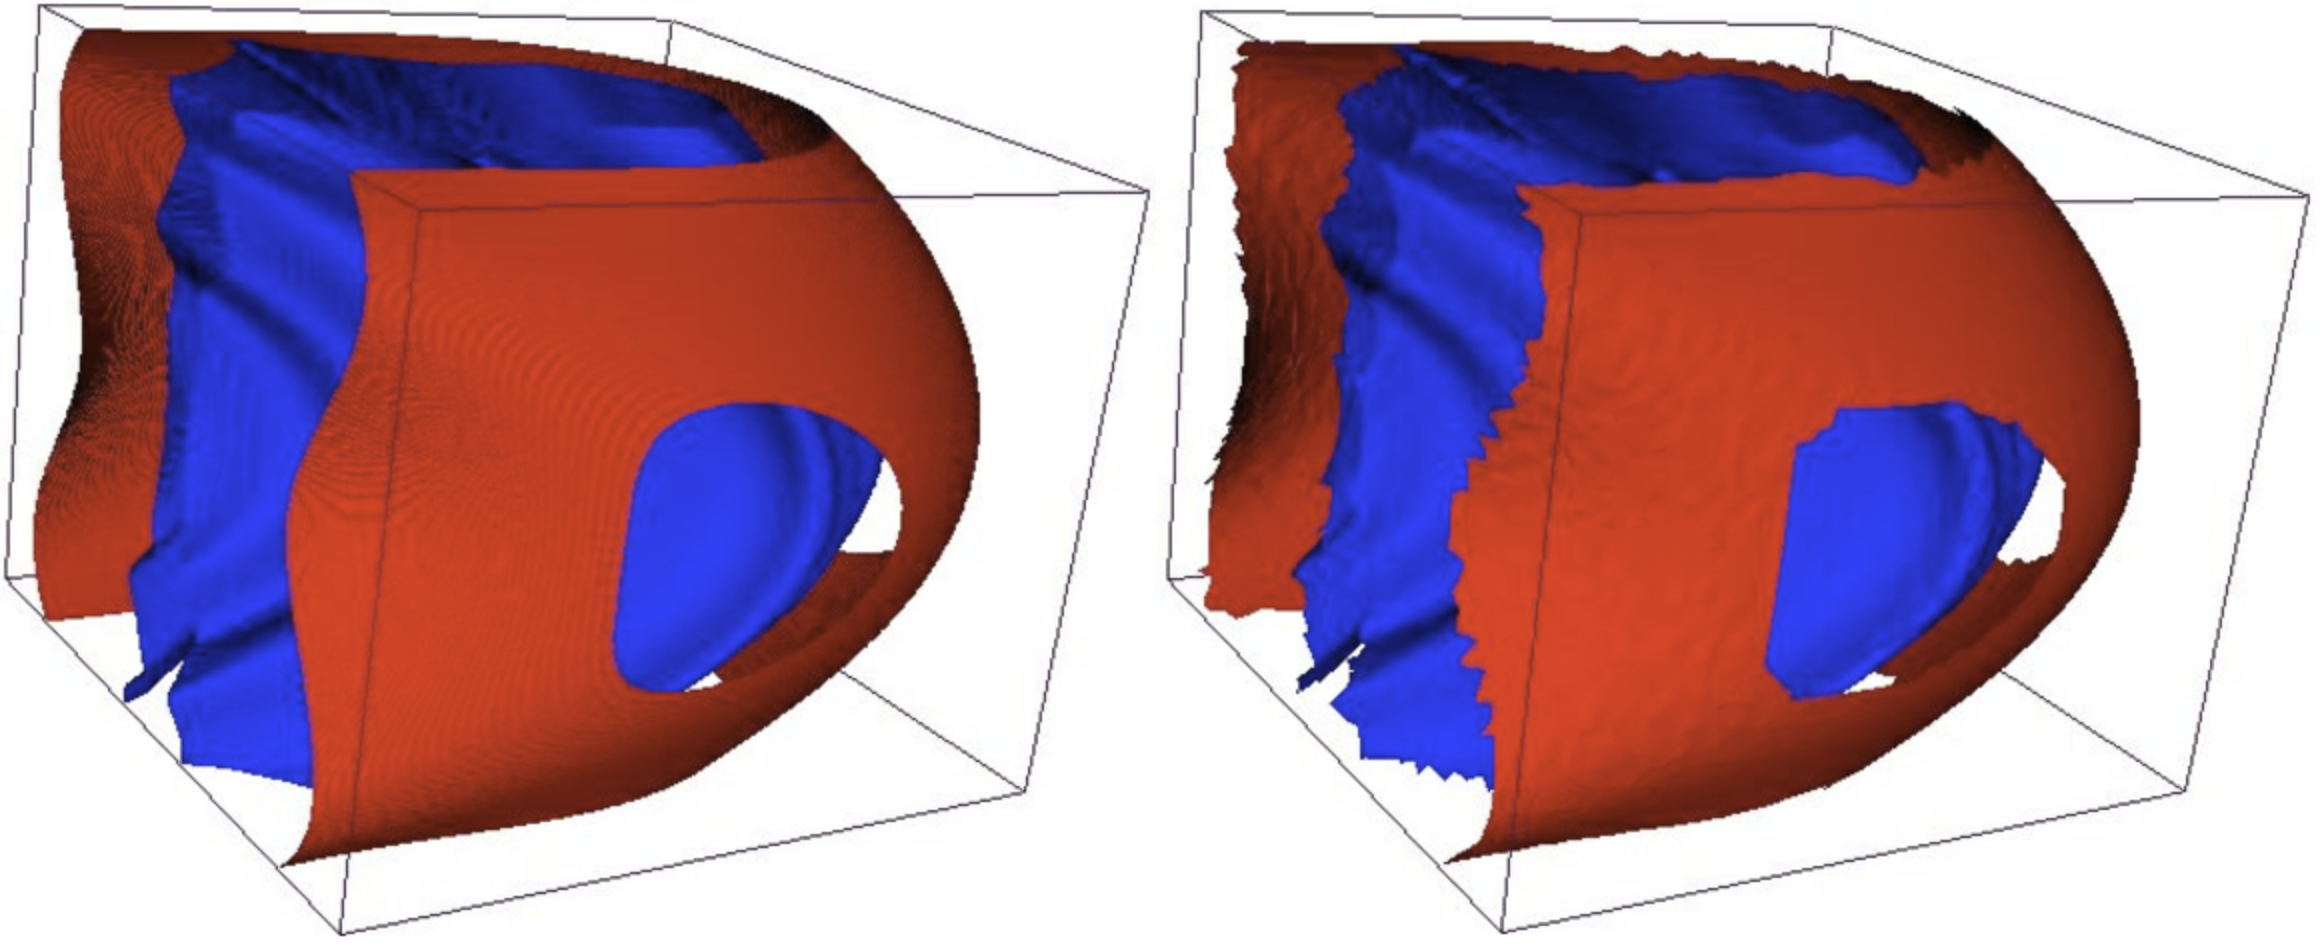
\includegraphics[width=0.6\linewidth]{figures/paraview.png}
    \caption{An example of a level-of-detail technique specified by ParaView. The model on the left is rendered at a higher resolution than the one on the right. While the quality of rendering is impacted, but improving rendering performance by having a lower resolution model to visualise.}
    \label{fig:paraview}
\end{figure*}
% multi-resolution representations or mipmaps as well as parallelism can be used to improve both visualisation and rendering performance
% describing and exploratory mode (a graphical user interface toll is used to explore the dataset) and batch mode (scripting and programming languages are used to write and execute a program

% portability - for to function on the diverse computational resources available and differnt displays (VR)
% accessability - ability to gain access to, setup, and run the tool
% extensibility - ability to easily add new functions to the tool
% describes a large dataset as data that exceeds the resource limit of a single machine
% uses a layered architecture
ParaView uses a layered architecture~\cite{Ahrens2005}.
The VTK foundation layer handles the data representation and algorithms~\cite{Ahrens2005}.
The second layer handles the parallel extensions to the visualisation toolkits, while supporting streaming of many data types and parallel execution.
The third and final layer is ParaView itself, which provides a graphical user interface and the visualisations.

\subsubsection{Astronomy Data Visualisation Systems}
Among the systems used to process and visualise \textit{big data} datasets there are some systems exclusively made for astronomy data.
% \cite{Lan2021}
% a comprensive catalogue of the current state of visualisation technologies present in astrophsyics

\paragraph{CARTA}
The acronym CARTA stands for Cube Analysis and Rendering Tool for Astronomy~\cite{Comrie2021}.
% aim is to provide a usable and scalable system utilising modern web technologies and parallel computing
Its objective is to provide a usable and scalable system using modern web technologies,
and its main hallmark is being able to load and render a dataset of several Terabytes in a matter of second.
It achieves this by storing the dataset at various levels of resolution and sending only the required requested data to produce a comprehensible rendering, instead of attempting to render the whole dataset at once.
% hosts large datasets remotely, uses the remote approach
It makes use of the client-side remote rendering approach for handling large datasets, by hosting them on a remote server.
% access the remote data from a local web-based client
A local web-based client accesses the data through a network connection, the data is transferred to the client and rendered within the web browser.
% focuses on being able to load a dataset of several TeraBytes worth of data in a matter of seconds
% designed for the ALMA, VLA, SKA pathfinders
It is designed for the ALMA, VLA, and SKA pathfinders
% works with data types such as FITS, CASA, MIRIDA, and HDF5
and works with data types commonly used in astronomy research such as FITS, CASA, MIRIAD, and HDF5.

\paragraph{i-DAVie}
This software for data cube exploration within a virtual environment, 
providing tools to navigate and interact with the visualisations.
Functionality to view metrics and interactively mask regions of data in the VR environment to catalogue sources is particularly useful.
% They enable a unique and immersive perspective on the data and allow intuitive interactions with the data
The VR environment integration enables a unique and immersive perspective of the data, affording intuitive interactions.
% created using the Unity game engine
It was created using the Unity game engine and uses the client-server architecture within its design~\cite{Marchetti2020}.
% system design uses the client-server model with server side rendering, where the visualisation is generated on the server and the frames are streamed to the front-end
It stores the datasets on the server but also renders the visualisation using the server.
% takes computational load off of the client but adds latency to the inteactions
% This approach takes computational load off the client but adds latency to the visualisation feedback as the user interactions must first be sent to the server, then visualisation is then updated based on the received interaction, and finally the frames are sent back to the client.
% The latency is proportional to the distance the client is from the server, and therefore latency increases as the distance between the client and server increases.
%   interactions performed on the client is sent to the server
%   visualisation is udated based on the input
%   frames are sent back to the client
A prototype system similar to i-Davie created for public outreach~\cite{Ferrand2018}, is a tethered standalone system which means that the server and the client are connected to each other with a physical connector such as a cable.
It also uses Unity with custom scripts to visualise FITS files and displays the visualisation in a VR environment using the HTC Vive. 
It can produce iso-surface or volumetric visualisations of a dataset.

\paragraph{Frelled}
A general-purpose astronomy viewer~\cite{Taylor2015} which uses a set of Python scripts to create three-dimensional visualisations of FITS files inside Blender, and is used for visual source extraction, cataloguing, and analysis.
It can visualise large datasets of roughly 600,000 points at more than 10 frames per second, while providing tools to mask data interactively, functionality similar to i-DAVie.
The FITS file can be explored in a three-dimensional space, instead of two-dimensional slices.
It provides a significant speedup in source cataloguing compared to other viewers, facilitating the recording of hundreds of sources a day.
Visual source extraction by an astronomer is still currently more effective than automated processes.
% motivations
%   desire to view 3D datasets in a 3D space
%   the need to rapidly mask regions of the data

\paragraph{AstroBlend}
A Python package for Blender~\cite{Naiman2016}, combining the three-dimensional capabilities of Blender with astronomy analysis tools.
Allows astronomers to analyse data alongside visualisations, while simplifying the importing process.
% simplifies the importing process of importing astrophysical datasets, generating visualisations, and anyalysis plots

\paragraph{SlicerAstro} % other good sources
A multi-platform open-source package for visualising and processing medical images,
which is an extension of the open-source software 3D slicer~\cite{Fedorov2012}.
It aim is to provide an interactive three-dimensional visual analytics tool using two-dimensional displays and interaction devices.
It is implemented using C++.
Its features include interactive filtering, three-dimensional masking and modelling, and support for FITS files.

\paragraph{E0102-VR}
\cite{Baracaglia2019}
An experimental standalone application using a VR display and interaction devices.
Its aim is to demonstrate the benefits of using human depth perception for fast and accurate characterisation of three-dimensional structures.
It explores the scientific potential of VR for displaying multi-dimensional datasets in astronomy and astrophysics.
The system pre-processes datasets into an iso-surface representation as it does not currently support volume rendering.
These pre-processed datasets can be swapped out with no effect on the functionality, but the system is currently coupled to a single dataset (SNR E0102) for experimental purposes.
The size of the dataset is limited because all the computation is done on a single computer.
% the pre-compiled/pre-processed dataset can be swapped out with no major loss of functionality
%   currently coupled to a single dataset (SNR E0102) for experimentation purposes
% uses isosurfaces to represent the visualisation
% limits the size of the datasets that can be used as all computation is done on a single computer
\subsection{Findings}
\label{sec:findings}
% VR findings
Virtual reality technology has made significant strides since its conceptualisation, evolving into immersive experiences that blur the lines between real and virtual environments. 
Central to the effectiveness of VR experiences are the concepts of presence, interactivity, and immersion. 
Presence is the sensation of physically existing within the virtual world, influenced both by subjective perceptions and objective indicators. 
Interactivity allows users to engage dynamically with the virtual environment, enhancing their sense of immersion and agency. 
Immersion, with its cognitive, emotional, kinesthetic, and spatial dimensions, contributes to a rich user experience across various platforms. 
Challenges such as simulator sickness highlight the importance of high-performance hardware in maintaining immersion and preventing adverse effects. 

% interaction is also very important in visual analytics
% interaction creates a much deeper experience for the user whether it is for entertainment or knowledge extraction

% Thus, interactivity serves as a crucial determinant of the overall quality and effectiveness of the user experience, shaping the user's sense of presence, immersion, and agency within the digital realm.
% Simulator sickness can affect some individuals but can be diminished 

% visual analytics key findings
% progressive rendering benefits both rendering effeciency and visual analytics

% The user explores the data from a broad overview and refines there search through continually adjusting the subset of data as they explore.
% From a system efficiency perspective the broad overview is a down-sampled data cube and as the user explores higher resolution portion of the data-set is brought to be visualised.
% Decreasing the time which the user is waiting for the visualisation as well as decreases the computational load on the system by limiting the amount of data visualised at any point in time.

The integration of visual analytics into data exploration and analysis practices offers a dynamic approach to uncovering insights and patterns within datasets. 
Through visual representations, analysts are empowered to interact with data, leveraging their inherent pattern recognition abilities to extract knowledge effectively. 
% For a data-set to be explored effectively there must be some way of interacting with it to facilitate exploration.
% This is to aid in extracting knowledge from the visualised data-set, and is imperative to the users ability to extract data from a visualisation
% Whether exploring to construct hypotheses, analysis to validate conjectures, or presentation-focused visualisation for effective communication, 
The goal of visual analytics is to enhance analytical reasoning and research through interactive visualisations. 
The efficacy of visual analytics hinges on user interaction, where progressive visualisation plays a pivotal role. 
It benefits both the flow of exploration for the user as well as the overall functionality of the system.
By allowing users to steer the representation's progress through data exploration, it facilitates a seamless transition from low-fidelity overviews to detailed insights. 
This iterative process, supported by techniques such as zooming, filtering, and immersive experiences like VR, enables analysts to navigate complex datasets efficiently. 
VR offers a compelling avenue for immersive analytics, providing an intuitive environment for multi-dimensional visualisations. 
By bridging the gap between quantitative data and human perception, VR not only enhances interaction but also enriches the understanding of complex phenomena, fostering a more holistic and user-centric approach to data analysis.

% data visualisation key findings
% explores how volumetric data can be rendered on a display
% Volumetric data can be represented as a visualisation using many different techniques, such as points, splats, iso-surfaces, and volumetric rendering.
% Each technique varies in how much computational resources is required to generate a visualisation.
% compares techniques such as points, splats, iso-surfaces, and volumetric rendering to determine the positives and negatives of each method
The data visualisation section \ref{sec:data-visualisation} also discusses the benefits of of using a three-dimensional visualisation rather than two-dimensional views. 
The visualisation of volumetric data cubes, particularly in fields like astronomy, presents a challenge because the complexity and scale of the datasets involved. 
These data cubes are essential for understanding phenomena in various scientific disciplines, including astronomy, medicine, oceanography, molecular-modeling, and engineering. 
Visual representation techniques unlock insights from these datasets.

One of the key objectives of data visualisation is to enable users to explore and understand complex data more deeply while having the means to communicate their findings to others. 
However, the unique characteristics of radio astronomy data, such as its massive size and dynamic range, present specific challenges for visualisation.

Various visualisation techniques exist, each with its own advantages and limitations. 
These include points, splats, iso-surfaces, and volume rendering. 
Among these, volume rendering emerges as the most comprehensive method for representing volume data, providing a detailed view and of external surfaces and internal structures within the dataset. 
It is resource-intensive, volume rendering offers a robust approach for extracting knowledge from volumetric datasets.

Furthermore, the choice between two-dimensional and three-dimensional visualisations is crucial. 
While two-dimensional approaches may be enough for certain analyses, three-dimensional visualisations are generally more effective for representing volumetric datasets comprehensively. 
They reveal hidden features and allow for a more intuitive understanding of the data, enhancing communication of quantitative results.

In summary, effective visualisation techniques are unlocking insights from volumetric datasets in fields such as astronomy. By leveraging advanced visualisation methods like volume rendering and prioritising three-dimensional representations, researchers can better understand complex data and communicate their findings more effectively.

% rendering strategy key findings
% In the rendering strategy section it was found that it is not enough to simply scale the computational power of a system as the size of data cubes increase, there is a need for a more intelligent strategy to handle the increasing size of the data cubes.
% It is very inefficient to simply brute-force the generation of visualisations by throwing more computational resources at the issue.
% The size of the data cubes are increasing in size at a faster rate than the development of the computational power of system, especially devices made for commercial consumption by the mass market. % see if i can find a source for the increase of data in astronomy and computer power
The rendering strategies section addresses the challenges of visualising large datasets and the strategies that balance computational efficiency with maintaining data integrity and user experience. 
Traditional approaches, such as brute force visualisation, strain computational resources and impede real-time interaction. 
To overcome these limitations, progressive visualisation techniques, used by i-Davie, offer a solution. 
By presenting users with initial down-sampled overviews and enabling them to explore areas of interest in greater detail, these methods optimise processing time without sacrificing accuracy or overwhelming users with excessive information. 
Moreover, remote rendering strategies, whether server-side or client-side, offer avenues for offloading computational overhead and accommodating datasets larger than the client's resources can handle. 
However, network bottlenecks and trade-offs between data compression and integrity must be managed carefully to ensure efficient data transfer and timely user feedback. 
As datasets continue to grow in size, the development of scalable visualisation systems that prioritise both performance and usability remains imperative.

% explore current system which work on the problem of visualising very large volumetric data-sets
% current systems key finding
% Some of the current systems that were reviewed produced some key points.
% Such as the benefits of pre-processing large datasets where the system retrieve higher detail versions of a section of data to provides a speedup with data visualisation.
% Three-dimensional representations produce a better experience for viewing multi-dimensional datasets and VR displays provide a more intuitive experience when working with multi-dimensional datasets than two-dimensional displays.
% VR technology also leverages user depth perception and spatial awareness.

% In some current astronomy visualisation systems they attempt to use datasets in the FITS file format to create 3D visualisations. 
% Implementations produce effective three-dimensional visualisations, however, the Fits file format is not suited for efficient visualisation as the data is stored in sequential slices, like pages in a book. 
% This makes traversing and extracting data to create the three-dimensional visualisation tedious. 
% Files can also be too large to be visualised as a whole and whole have to be broken up into more manageable pieces for visualisation.
% Breaking datasets into pieces runs the risk of obscuring the context of the individual piece and could obscure the insight the dataset would communicate as a whole.

% While building the experimental system E0102-VR~\cite{Baracaglia2019} some insights were found involving the use of VR for viewing and interacting with multi-dimensional datasets.
% The depth perception provided by VR aids in understanding complex three-dimensional structures and provides means to quickly measure distances and angles in three dimensions.

The review of existing systems has highlighted several key points. 
For instance, the advantages of pre-processing large datasets, where systems retrieve higher-detail sections of data to expedite data visualisation. 
Three-dimensional representations enhance the viewing experience for multi-dimensional datasets, and VR displays offer a more intuitive interface compared to two-dimensional displays. 
VR technology capitalises on user depth perception and spatial awareness, further improving the visualisation process.

Efforts have been made to utilise datasets in the FITS file format to generate 3D visualisations, in system such as \textit{Frelled} and \textit{SlicerAstro}
While these implementations yield effective three-dimensional visualisations, the FITS file format is not inherently conducive to efficient visualisation because of its storage of data in sequential slices, like pages in a book. 
This sequential storage method makes traversing and extracting data for three-dimensional visualisation a cumbersome task. 
Additionally, files may be too large to visualise in their entirety, necessitating the division of datasets into more manageable pieces. 
However, breaking datasets into fragments risks obscuring the context of individual pieces and potentially diluting the insights the dataset would otherwise convey as a whole.

During the development of the experimental system E0102-VR, valuable insights were gained regarding the utilisation of VR for viewing and interacting with multi-dimensional datasets. 
The depth perception afforded by VR aids in comprehending complex three-dimensional structures and facilitates rapid measurement of distances and angles in three dimensions.

\newpage
\section{System Design and Implementation}
\label{sec:system-design}

% NB be more abstract in this section
% it sounds like you are talking about something that has already been made

% have a diagram of the system at the to
% following paragraphs explain the components
% any diagrams relating to those components go in these paragraphs as well

% explain why we use stuff in the introduction, give context

% explain how everything works in the respective subsection

% what does VRDAVis do
% it visualises large astronomy datasets
% using a server to store and process the data and a client to display the data and allow th user to interact and explore the data through a visualisation
% the server is accessible through the internet
% the client is also accessible through the internet
% the client functions within a web browser
% the client can function on a desktop computer such as a laptop or on a standalone VR headset such as the oculus quest 2

This section explains the design and implementation of the VRDAVis system. 
It outlines the system's structure and delves into how each component functions, some key language and package choices, as well as some key algorithms. 
The full source code can be found at the public GitHub repository for VRDAVis~\cite{VRDAVisGitHub}.

% libraries used in project
The architecture of CARTA was used as a guide for architectural choices and implementation. 
VRDAVis is a prototype proof-of-concept system, with the goal of potential integration into CARTA as additional functionality. 
The architecture was kept as similar as possible to allow the systems to be integrated with minimal changes to both systems.
% explain client-server architecture
%   server -> hosts, delivers, and manages most of the resources and services requested about the client
%   client -> presentation

% colour code diagram
\begin{figure*}
    \centering
    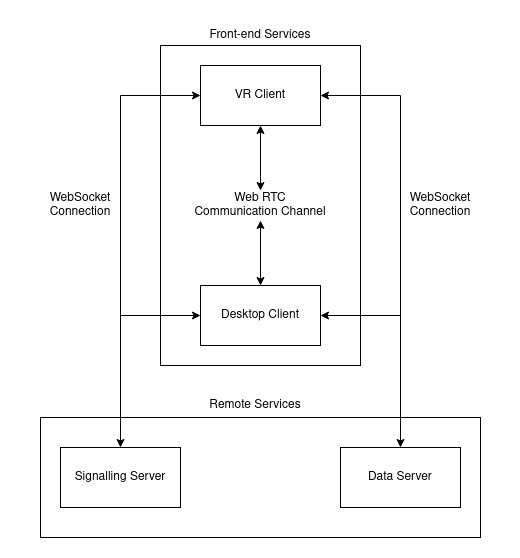
\includegraphics[width=0.6\linewidth]{figures/system-diagram.jpg}
    \caption{The VRDAVis high-level system architecture, showing the front-end and remote services. The arrows depict communication channels between the components, where the main channels of communication are between the client of the front-end services and the data server of the back-end services, the front-end client and the signalling server, and the VR and Desktop clients.}
    \label{fig:system-diagram}
\end{figure*}

The system uses the client-server architecture. 
With two main subsystems, the front-end and remote services.
The front-end service only contains the client web browser application.
This application is used on both the desktop computer and the standalone VR headset. 
These remote services host, deliver, and manage the resources and services requested by the client. 
% The data server and the signalling server sub-systems are separate remote systems which serve the client application. 
% The front-end services controls the majority of the system logic, while also being the main point of interaction between the data visualisation and the user. 

% The rendering approach, where a system like VRDAVis renders the data visualization on the client instead of the server, is referred to as client-side rendering. 
% A more in-depth explanation about the rendering approach can be found in Section \ref{rendering-strategy}.

Several libraries were evaluated for the development of VRDAVis. These included libraries for embedding VR environments and rendering three-dimensional graphics in a web browser, web-socket and peer-to-peer connections.
Aspects of these packages and libraries such as functionality, documentation, community support; must be considered before attempting to integrate.
Selecting a sub-optimal package which is not suited for the needs of the system could have potential cascading effects on the overall design of the system and the project timeline.
Many of the architectural and system choices were selected because for compatibility with CARTA's architecture, the relevance of each choice will be explain further in the respective sections.

% More details about the respective subsystems are explained in the sections below.

The main decisions in designing and implementing this architecture is deciding which system function are performed by the respective services. 
Once the system has been implemented, moving a task to a different service could be costly. 
For this prototype system, only one architecture could be tested, because of time constraints imposed on this research project.

% breifly explain the components of the system and how they work with each other
% the user side manages system logic and user interaction

The remote and front-end services, with their respective components, work together to create VRDAVis. 
We explain the functionality starting with front-end service, where the user begins their interaction with VRDAVis.

The web browser application is accessible through the Internet, either on a desktop computer or on a standalone VR headset. 
The interface allows the user to choose from a list of files available on the data server. 
These files are pre-processed HDF5 files that store data at various levels of resolution. 
This allows the browser application to request the same section of a data cube at a higher or lower resolution, and then display the requested data for the user to interact with.

The user can use the file selection UI on a desktop computer or a VR headset, but the embedded VR environment can only be accessed through the browser on the VR headset. 
Once the file has been selected, a low-resolution version of the entire data cube is requested from the data server. 
The data is sent from the data server to the browser application, where it is rendered into a visualisation. 
The visualisation can be viewed from the browser window or from within the VR environment.

However, if the user is viewing the visualisation from a desktop computer and would like to view it from a VR headset, the state of the visualisation can be transferred to the VR headset, and vice versa.
This process uses a peer-to-peer connection between the two devices to transfer the application's state. 
This connection is facilitated by the signalling server, which assists with the pairing of the devices as well as automatically establishing a new peer-to-peer connection. 
The signalling server itself is not involved with the data transfer once the connection is established.

Once the user has entered the VR environment, they can interact with the visualisation using various actions like translation, rotation, and scaling. 
If the user wants to examine a portion of the data cube in more detail, they can select the crop mode from the menu and draw a cube around the portion they are interested in. 
Once the area has been finalised and the crop button has been selected, the application determines which cubelets to request from the data server. 
As they arrive, they are reassembled into a larger cube and rendered. 
The user can continue to select and crop smaller portions of the visualised cubes until they reach the highest resolution level available for the selected file.

\subsection{Communication Layer}
\label{sec:communication-layer}
% introduction to communication layer
The sub-systems of VRDAVis need communication channels and protocols to communicate effectively.
These channels are established between the components of the front-end service and remote services. 
The data and signalling servers within the remote services communicate with the client application in the front-end. 
Peer-to-peer connections are formed between instances of the client within front-end services. 

\subsubsection{Data Server and Desktop/VR Client Application}
The communication between the user-side browser application and the server-side data server takes place through a WebSocket connection, which is more suitable for VRDAVis than the typical request and response or promise and resolve model common in many HTTP-based clients and servers~\cite{MDN_WebSockets_API}.
WebSockets allow the respective systems to send messages to each other without requiring a request first to respond. 
This behaviour allows for many responses to a single request, 
so the server is not restricted to responding to the client with a single very large message with a large piece of data, it can send smaller pieces of data in individual messages.

Protocol Buffers are used to define the structure of messages and facilitates the reading and writing of structured data to and from various data streams using different programming languages, such as C++, JavaScript, and Python.
The Protocol Buffer library was created by Google to serialise structured data. 
A platform-neutral mechanism for converting data objects into a byte stream for transfer~\cite{Google_Protocol_Buffers}.
This library is used to define a schema and format for data exchanged between the front-end and remote services. 
The Protocol Buffer message definitions are stored in their own folder and are used by the user-side and server-side systems. 
When a message needs to be sent from the user-side to the server-side or vice versa, the data objects are serialised into a byte stream before they are transferred. 
Once the data arrives, it is converted from a byte stream back into a data object.
% serialisation -> process of converting data type objects into a byte stream for transfer
IProtocol Buffers was chosen for its error-prevention capabilities compared to JavaScript Object Notation (JSON), and because it is the chosen communication format used in CARTA.

\subsubsection{Signalling Server and Desktop/VR Client Application}
The signalling server creates, manages, and establishes peer-to-peer connections between instances of the client browser application on different devices.
% JSON
The communication required between the signalling server and the client application is significantly less complex than the communication between the data server and the client application.
The tasks performed by the signalling server are also less time-sensitive than those performed by the data server, and less data needs to be transferred between them.
These factors led to the use of the simple request-response communication protocol to be used as well as the use of JSON to format the messages.
JSON is a lightweight format for storing and transporting data that is language-independent and easy to understand as it considered ``self-describing"~\cite{JSON}.

\subsubsection{Client Application and Client Application}
Another component of the communication layer is the peer-to-peer connection between two instances of the client web browser application. 
One of these instances would be in a browser on a desktop computer, and the other would be in the browser on a standalone VR headset. 

Web Real-Time Communication (WebRTC)~\cite{Blum2021, WebRTC} is an internet communication protocol that enables web applications to stream audio, video, or data between peer browser windows, without the need for the data to be routed through an intermediate server. 
It facilitates peer-to-peer communication without requiring additional third-party packages.
% facilitates peer-to-peer without requiring plug-ins or third-party software to be installed
% support for audio and video conferencing, file exchange, screen sharing, identity management, and interfacing with legacy telephone
WebRTC is used in VRDAVis to establish a connection between these instances. 
This connection is used to transmit the application's state between its peers, allowing the user to continue their work seamlessly without needing to repeat steps on another device.
% used to create a peer-to-peer connection between browser instances on different devices
% used to send data between the broswer instances 
% chosen for its functinality to create peer-to-peer connections
% peer-to-peer connection
This peer-to-peer connection allows the instances to exchange data between instances without having to send it through middleware service such as a server. 
However, it does require the signalling server to establish and manage the connections. 

% has the capability with help from the signalling server to create a peer-to-peer conection between another instance of the client on a VR headset
%   show pairing process diagrams
%   show transfer diagram

\paragraph{Headset Pairing}
% To establish the connection both devices must connect to the signalling server which a server-side component which stores unique id pairs which.
The initial pairing process requires both of the VR headset and the desktop computer to be connected to the signalling server. 
When each devices connects, it sends the server an unique ID, a name, and announces whether it is a VR capable device. 
The server checks if the device already has a pair and if it does not find a pair it sends a list of unpaired VR devices to the unpaired devices which are not VR-capable. 
A desktop user selects a VR device and generates a code from the desktop computer, a code which is sent to the signalling server, and forwarded to selected device using its unique ID. 
The VR device then prompts the user to enter the code locally, and verifies it against the code received from the server.
When the server confirms that the codes match it saves the device pair to a local JSON database.
The server then sends a confirmation message to both devices stating that the devices have been paired.
Both devices then confirm that they are ready to begin a peer-to-peer connection and the WebRTC peer-to-peer protocol begins.

\begin{figure}
    \centering
    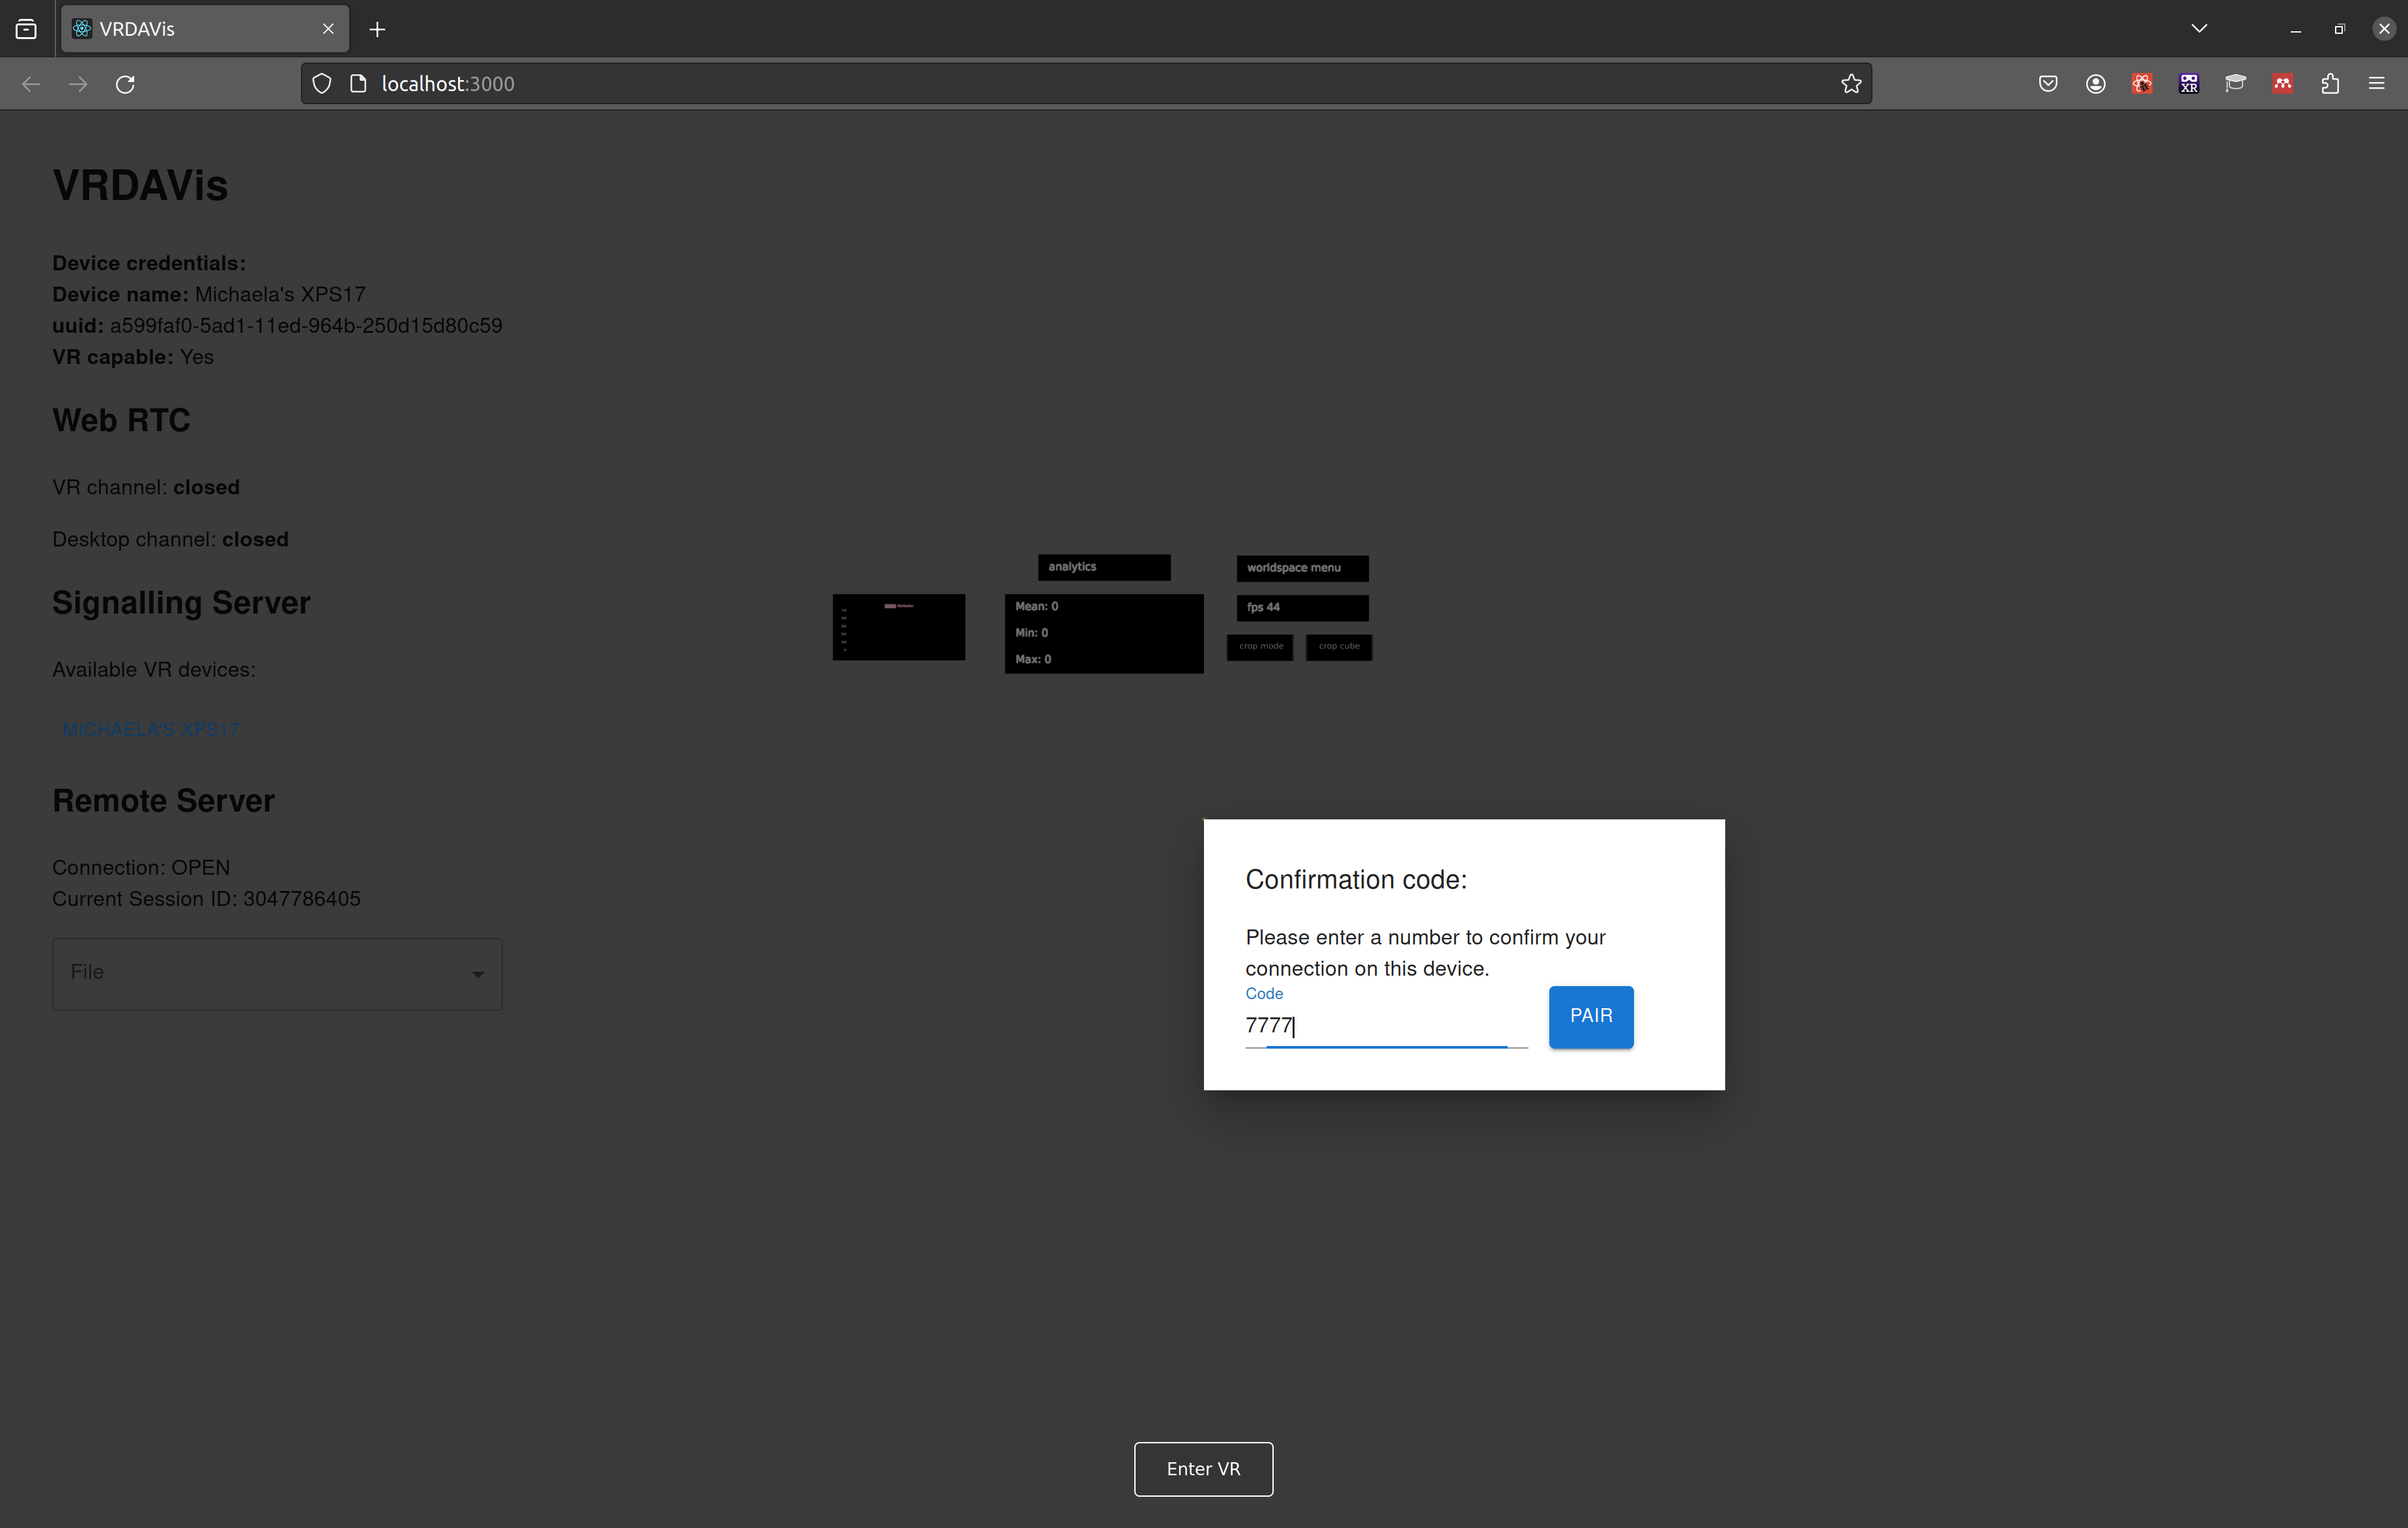
\includegraphics[width=\linewidth]{figures/screenshots/3.png}
    \caption{The menu that appears in the browser window when the user selects a VR device to pair with on the desktop computer. The user must enter a code which must also be entered in the same menu on the VR headset.}
    \label{fig:screenshot-3}
\end{figure}

% pairing process diagrams
\begin{figure*}
    \centering
    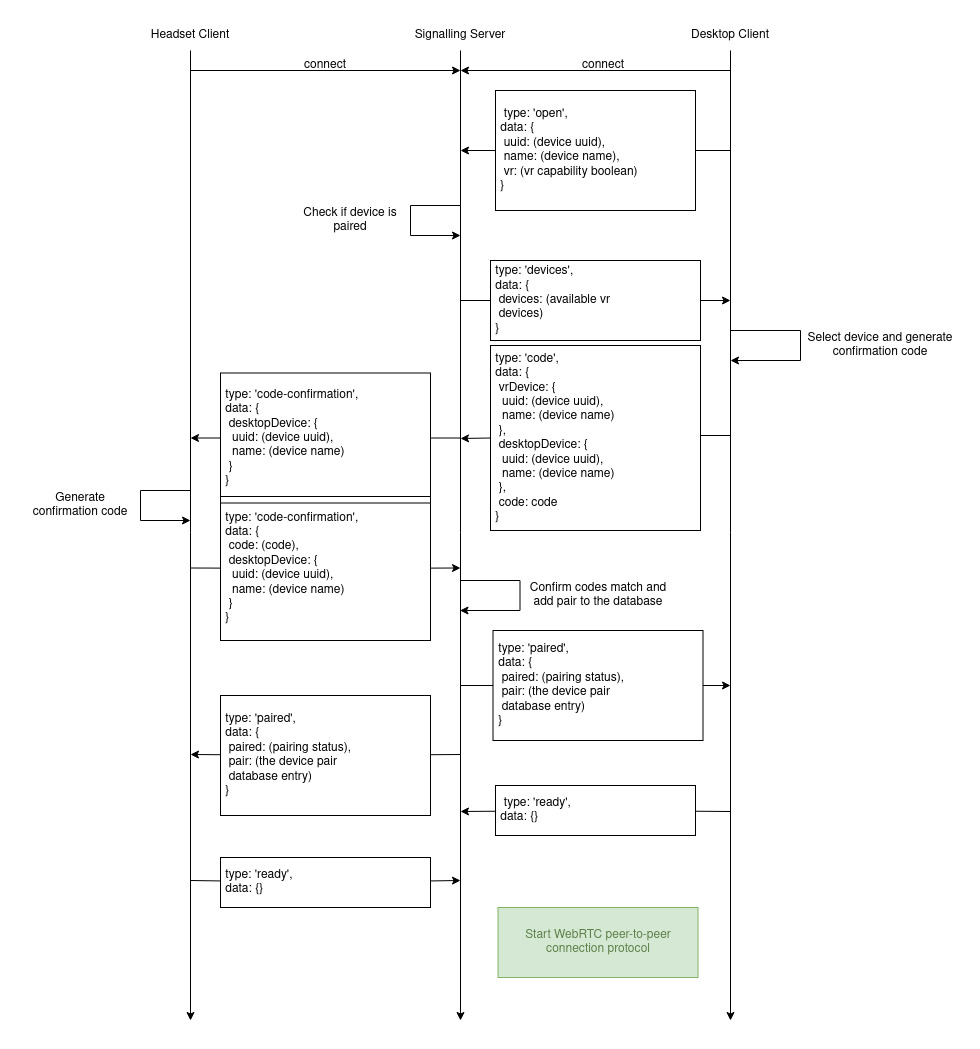
\includegraphics[width=0.6\linewidth]{figures/pairing-process.jpg}
    \caption{The pairing process between an instance of the front-end application running on a desktop computer and an instance running on a VR headset. It shows the order of the messages sent from each device and the contents of each message.}
    \label{fig:pairing-process}
\end{figure*}

\paragraph{Paired Devices Connection}
% Once the devices have been paired they must connect to the signalling server at the same time and then a peer-to-peer connection is established between the paired devices. 
% No data which is sent between the devices on the peer-to-peer connection passes through this server.
When one device connects to the signalling server, the server checks if the device is currently paired by searching the JSON file which contains all the pairs.
If the device is paired, the server checks if the other paired device is connected to the server as well.
When the VR device and the desktop computer are connected to the signalling server and the server detects that these device are paired to each other, it starts the process of creating the WebRTC peer-to-peer connection.

\begin{figure*}
    \centering
    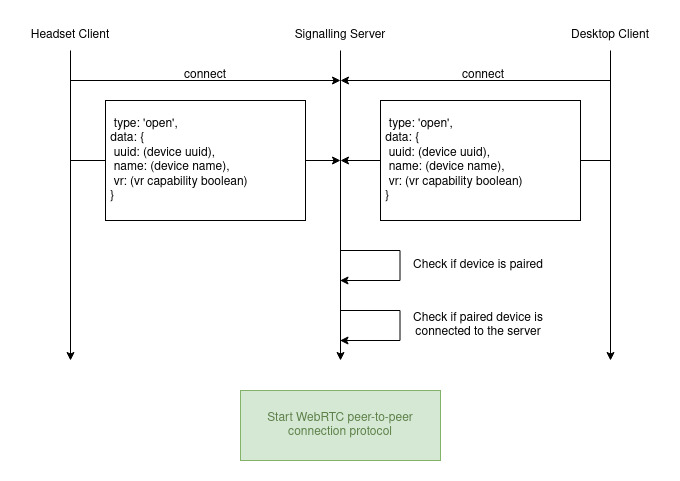
\includegraphics[width=0.6\linewidth]{figures/connect-paired-devices.jpg}
    \caption{The process of connecting paired devices through the signalling server. Both devices indicate that they wish to open a peer-to-peer connection with their ``open" messages.}
    \label{fig:connect-paired-devices}
\end{figure*}

\paragraph{Peer-to-peer Connection}

Once the VR headset and the desktop client indicate that they are ready to establish a peer-to-peer connection with each other,
the desktop client sends WebRTC Interactive Connectivity Establishment (ICE) candidates to the VR device through the signalling server.
These ICE candidates contain the protocols and routing needed for remote devices to communicate with each other as well as details used to establish the connection.
Multiple candidates are sent until one is found which works for both devices.
The candidates are sent to the VR device through the signalling server as this is the only channel currently connecting the devices.
The desktop computer creates a Session Description Protocol (SDP) offer, which contains the RTCPeerConnection interface. 
It contains information about open channels already attached to the current WebRTC session, a codec, any candidates already gathered, and options supported by the browser.
This SDP offer is sent to the VR device through the signalling server, and the VR device handles the offer through WebRTC by creating an answer which contains the corresponding information about its own capabilities.
The answer is returned to the desktop client, the offer is resolved and the peer-to-peer connection is established between the devices.
No further data needs to pass through the signalling server in order for the devices to communicate with each other; they now pass data to one another through the peer-to-peer connection.

\begin{figure*}
    \centering
    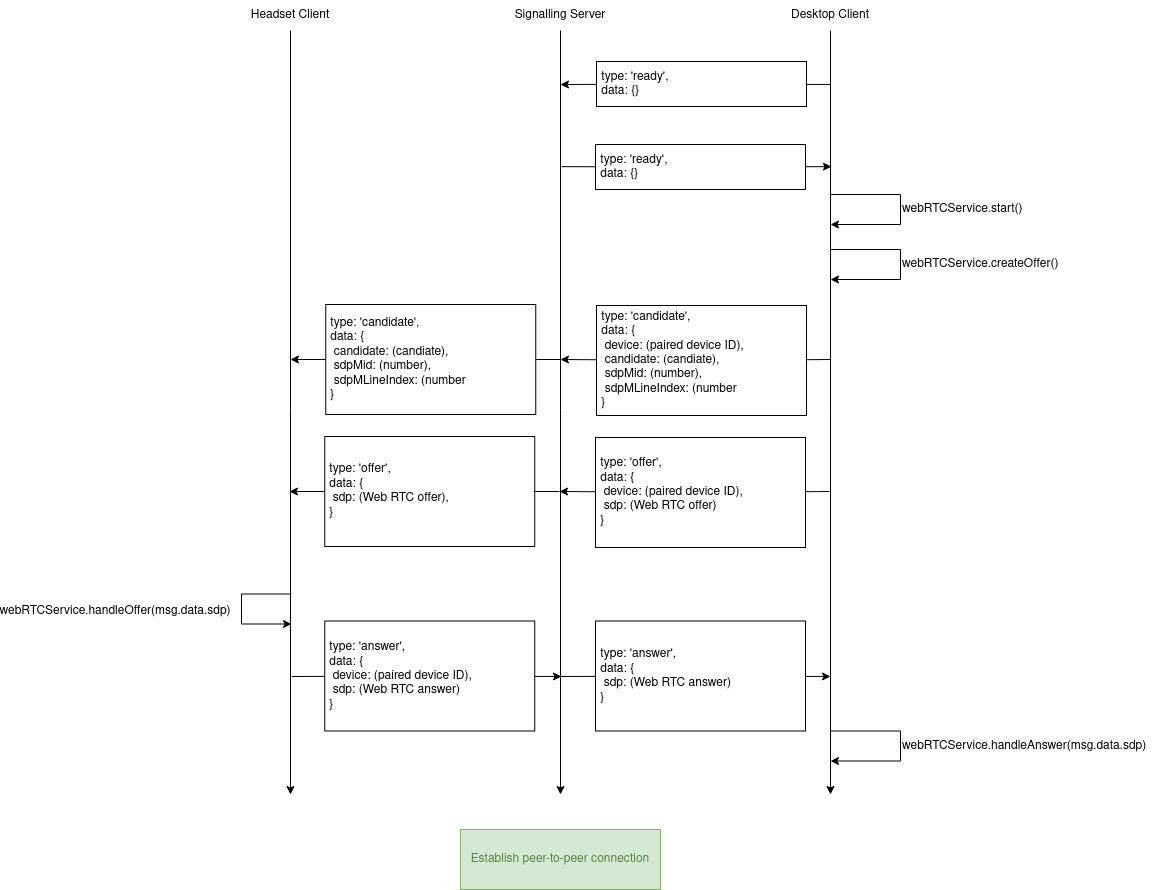
\includegraphics[width=0.8\linewidth]{figures/peer-connection(1).jpg}
    \caption{How the peer-to-peer connection is established between the paired devices.}
    \label{fig:peer-connection}
\end{figure*}

\paragraph{Transferring Client Application State Over Peer Connection}
The purpose of the peer-to-peer connection is for the connected instances of the front-end to exchange state.
This allows the user to start their exploration of a data cube on a device such as a laptop or a desktop computer, then move the state of the desktop instance to the VR headset to continue the exploration in the VR environment.
Transferring the state of an instance in this manner means that the user does not need to perform additional steps to start a new instance and get back to the same position in their new exploration.

The state is transferred through JSON messages sent over the peer-to-peer connection.
Each message contains the file name, and the size and the position of the local cube state.
Once these details have reached the new instance, a new connection to the data server is used to make requests and receive responses from.

% JSON
% add a diagram for how the state is transferred between the devices
\begin{figure*}
    \centering
    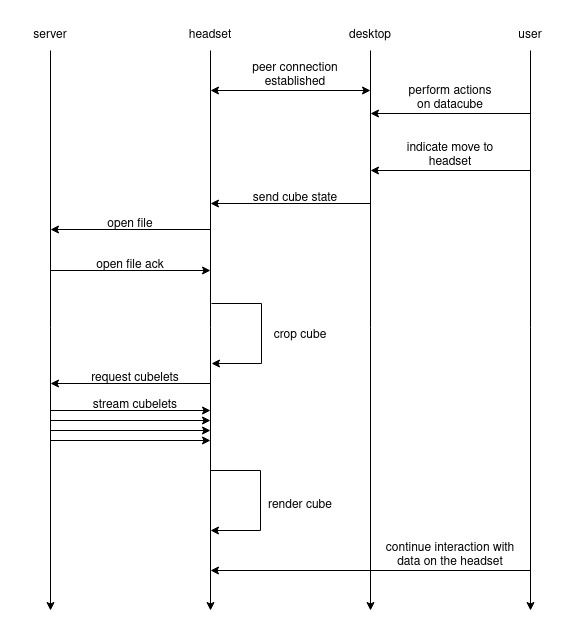
\includegraphics[width=0.6\linewidth]{figures/transfer-flow.jpg}
    \caption{The diagram depicts the event sequence for transferring the state between the two instances of the front-end browser application. The application state can be bilaterally transferred between client devices.}
    \label{fig:transfer-flow}
\end{figure*}

\begin{figure*}
    \centering
    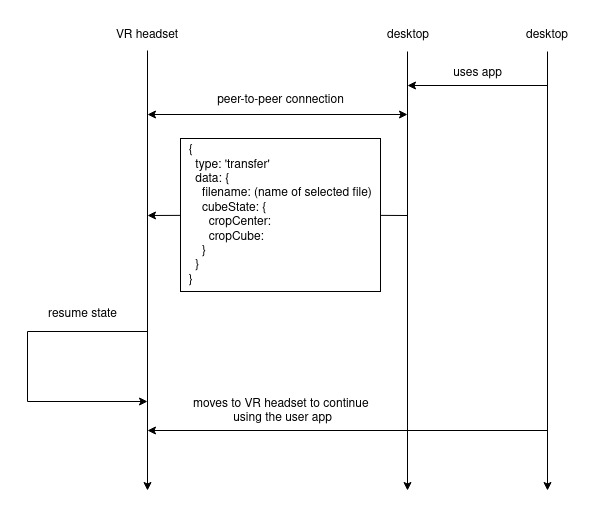
\includegraphics[width=0.6\linewidth]{figures/transfer-cube-state.jpg}
    \caption{The message structure which is sent between the VR headset instance and the desktop instance when the cube state needs to be transferred between the devices.}
    \label{fig:transfer-cube-state}
\end{figure*}

\subsection{Server-side}
\label{sec:remote services}

The remote services of VRDAVis are composed of all the systems that serve the front-end applications; consisting of a data server and a signalling server. 
The data server receives requests from the user application, where its purpose is to transfer data from astronomy data files. 
The signalling server is used to create and manage peer-to-peer connections between two instances of the front-end browser application. 
The peer-to-peer connection is used to transfer the state of the visualisation across instances, allowing the user to transfer the state from a desktop computer to a standalone VR device and vice versa. 
This showcases how VRDAVis would be able to integrate into an astronomer's workflow with minimal disturbance.
% The main purpose of the server-side systems is to serve requests from the front-end clients. 

\subsubsection{Data Server}
% preprocessed files
% cite the CARTA HDF5 papers
% point out that there is a converter from FITS to HDF5
It is common in astronomy for data to be stored in the FITS format.
But in VRDAVis the HDF5 file format will be used to store data. 
Unlike FITS files, where data must be read sequentially, the HDF5 format allows any part of the file to be accessed at any point in time. %cite
The HDF5 C++ library is used to read the files. 
Initially written in C, the C++ package encapsulates the Python code into a format that can be interfaced with C++.

However, merely using a more effective file type is not provide speed-up for creating a visualisation of the stored data. 
Especially when the data in the file is still at its original resolution and therefore its largest size. 
It has the potential to overwhelm the client device with the sheer amount of data it would need to process.
The full-resolution data must be processed into multiple levels of resolution, referred to as mipmaps. 
These mipmaps are contained in the same HDF5 file as the data at its original resolution. 
Portions of the mipmaped data are read, instead reading the full-resolution data, decreasing the likelihood of overwhelming a client device.
% mention that the FITS to HDF5 converter also does the mipmap conversions
% cite the git repo

The server stores the data files pre-processed into a mipmaped format.
This approach to handling \textit{Big Data} files allows the entire dataset to be visualised with less computational overhead, compared to rendering the full resolution dataset~\cite{Li2016}. 
It still allows the visualisation to maintain the overall context of the data, but as the data is explored, higher resolution versions of the same region can be swapped out to allow the user to observe the details.

% insert diagram of how the preprocessed cubelets are stored in the server
\begin{figure*}
    \centering
    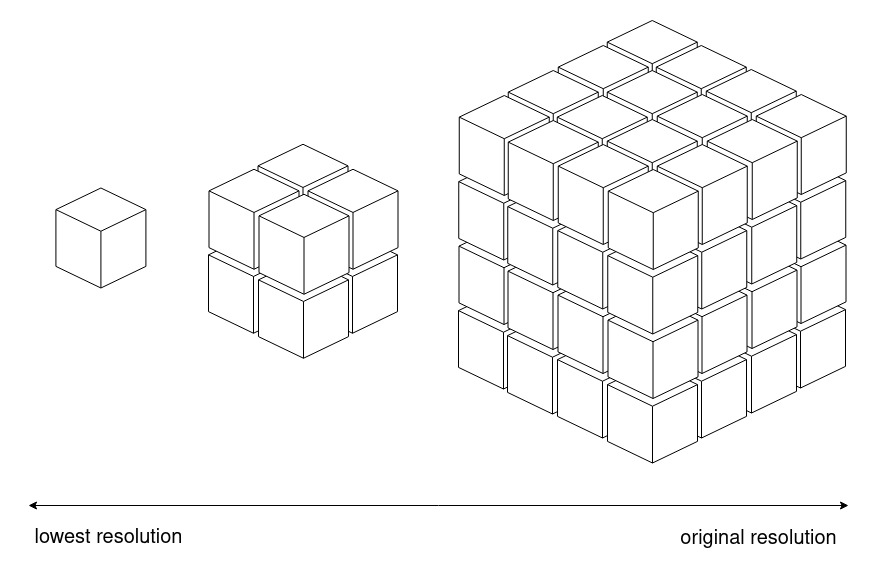
\includegraphics[width=0.6\linewidth]{figures/three-dimensional-mipmap.jpg}
    \caption{In the pre-processed data file, different resolutions are stored as mipmaps, from a single cubelet which represents the entire data cube to the original full-resolution data, with several intermediate levels.}
    \label{fig:three-dimensional-mipmap}
\end{figure*}

\begin{figure*}
    \centering
    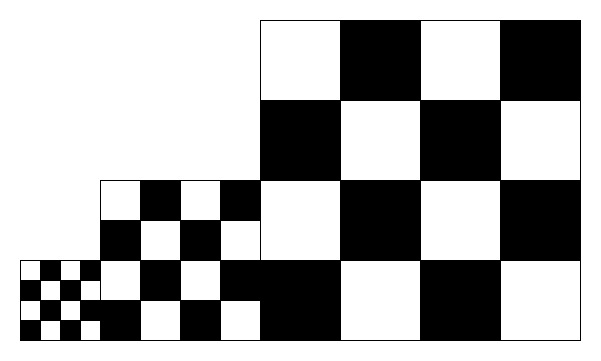
\includegraphics[width=0.5\linewidth]{figures/two-dimensional-mipmap.jpg}
    \caption{An example of a two-dimensional mipmap. Observe how the pattern is scaled at each level}
    \label{fig:two-dimensional-mipmap}
\end{figure*}

% mipmap
% \cite{Li2016}
% The displays on which the visualisations are rendered have a limited number of pixels, thus the lowest granularity possible is to plot one data point onto one pixel (Molina-Solana et al.2017; Olshannikova et al.2015; Yang et al.2015). 
% Visualisation tools are required to “squeeze a billion records into a million pixels”(Bikakis2018) empha-sizing the need for summarisation of data, particularly when creating visualisations

The server must fetch data from its filesystem according to the client's request. 
When the client requests a number of sub-sections of a data cube, the server retrieves these cubes or cubelets and streams them back to the client over a websocket connection. 
Each message streamed to the client contains one compressed cubelet. 
Additionally, the server performs file system functions such as sending lists of available files, opening them, and reading data.

The ability to view various analytics on the visualised data is also an important feature, and the server supports this by computing various derived values such as minimum, maximum, and median values. 
It also compiles analytics data to be visualised as various graphs, including the distribution of values.
%   fetches data based on the client's request
%       client requests a number of cubes but the server streams back the data in chuncks 
%       each message back to the client has the data of a single cube contained within it
%   file system functions (opening files and reading data from them)
%   performing analytics functions on data
% stores the data
%   the pre-processed mipmap data cubes as well as the full sized data cubes

The data server was written in C++ for the purposes of speed and performance and follows a similar structure to the CARTA software.
C++ is a high-level, general-purpose programming language used to implement the data server of VRDAVis remote services. 
An object-oriented programming language that was initially released in 1985 as an extension of the C programming language, with a focus on performance, efficiency, and flexibility.

It was selected for its speed of execution and object-oriented nature, as well as being the same language utilised in implementing the CARTA back-end.
uWebSockets is a C++ library used to integrate WebSockets into a C++ project.
It is also used establish WebSocket connections between the client application and the data server.

\subsubsection{Signalling Server}
Node.js, also referred to as Node, is a free, open-source server environment, with cross-platform capabilities, which uses JavaScript to create server-side tools.
It uses asynchronous programming which is a different manner to handle the conventional HTTP one request, one response model.
Synchronous systems wait for tasks to complete before returning content to the client, only once a task is complete is the system ready to handle the next request.
Asynchronous systems do not wait for a task to be completed before starting a new request.

VRDAVis uses Node in the signalling server to create and manage peer-to-peer connections between the instances of the front-end web applications.
It was chosen because servers can be implemented quickly.

Express is a minimal and flexible Node.js framework that provides a robust set of features for the development of web and mobile applications.
It is one of the most popular Node web frameworks.
% cite
It provides functionality to write handlers for HTTP requests at different URL paths know as routes.
It is integrated with view-rendering engines, which generate responses by inserting data into templates.
It has the functionality to set common web application settings like the connection port, and the location of templates.
It can also insert additional request processing known as middleware at any point within the request handling pipeline, to add functionality such as authentication.
It is used in the VRDAVis signalling server to implement the WebSocket connections, and was chosen because of its flexibility and the speed at which prototype systems can be implemented.

% from the comm section
% This server-side component is named the signalling server and is made using Node.js and JavaScript. 
% It also uses a WebSocket connection to communicate with the web browser application and sends dats using JSON. 
% Unlike the data server, this server component was not made with speed and performance as its main focus. 
% The speed of implementation was the focus when creating this component. 
% Its main purpose in the context of the VRDAVis system, besides creating the peer-to-peer connections, is to pair the devices, store the devices pairs, and streamline the connection process when the pair needs to reconnect.
\subsection{User-side}
\label{sec:user-side}
% give an overview of the user-side system
% a web browser application
The front-end service of the system is a user serving web browser application accessible through the internet. 
The decision to use a browser application ensures that application is operating system-agnostic, which makes it available to more user devices. 
It also allows the system to remain up-to-date with any changes for all users, unlike native applications, which the user is responsible for updating. 
% The front-end application is used on desktop computers and standalone VR headsets. 
The instances of the application can be used on desktop computers, laptops, and standalone VR headsets, and communicate through a peer-to-peer connection, which allows them to coordinate with each other without routing data through a server. 
These web application instances serve as entry points to the embedded VR environment, which can be accessed through the VR headset. 
This is the environment where the user can see the visualised data, interact with the visualisation, manipulate it, and explore.

React.js is the framework chosen to implement the web application for VRDAVis, to replicate architectural choices from the CARTA system, as CARTA also uses React.js for its front-end application.
It is a free and open-source JavaScript library is used for building user-oriented applications based on components and can be employed to develop single-page, mobile, or server-rendered applications. 
It is maintained by Meta and a community of individual developers as well as companies.

In addition to React.js, MobX is a state management library designed for front-end web browser applications, responsible for maintaining stateful information. 
It integrates into React and is also used for state management within the CARTA framework.

% explain how the mipmap data supports functionality on the front-end
% no unneccessary rendering of points which equate to smaller than a pixel
% it returns a managable amount of data
% does not overwhelm the computer with the sheer amount of data it needs to process

% hosts some of the system logic
The front-end also hosts the majority of the system logic as it determines which piece or pieces of data need to be retrieved from the server. 
When the initial data is retrieved or the cube is cropped, a list of cubelets must be made so that the correct subsections can be fetched from the appropriate resolution level. 
The resolution level and lists are determined through a selection process taking into account the predetermined cubelet size, cubelets are selected from a mipmap level which maximises the resolution while maintaining performance. 
It is biased towards the mipmap layer with the maximum downsample ratio, which reduces the total number of cubelets that cover a selected area, whether it is the whole cube or a subset of the cube. 
This strategy limits the maximum amount of data that can be sent to the client. 

This selection process is critical when the cube is cropped on the front-end, as it discards portions of the cube that are not being focused on. 
Figure \ref{fig:crop-cube} illustrates the relationship between the cropped portion of the cube and the cube space, showing the dimensions of the full-resolution cube, as well as how multiple cropping actions relate to each other. 
Each crop action selects a subset of the previous cube.

The algorithm used to crop the cube and select cubelets at a higher resolution level can be broken down into the several steps:
\begin{enumerate}
    \item To determine which cubelets need to be requested initially, the full-sized data cube is cropped with a selection boundary of the same size.  The cube localspace is the current state of the cube being visualised on the front-end application, and the crop cube is the subset of the cube for which higher resolution cubelets are going to be requested.
    \item Every time the cube is cropped, the visualised cube's space and crop cube's space are aligned in the full-resolution cube's space, which can also be referred to as the cube's worldspace, encapsulating the full resolution dimensions. This is done to ensure that the crop cube's corner coordinates fall within the x, y, and z dimensions of the cube's coordinates. This is achieved through the multiplication of the crop cube dimensions and the centre coordinates by the current mipmap level. The initial mipmap level for the XY and Z axes is set to 1, and when the cube is cropped, the cube localspace dimensions and centre are updated to equal the crop cube's dimension and centre.
    \item The corners are calculated by the division of the dimensions by 2 then the addition or subtraction of this number to the centre for the x, y, and z dimensions.
    \item The crop cube's dimensions and centre are translated to coordinates within the full-resolution cube.
    \item The maximum mipmap level that data can be fetched from is determined by the adjustment of the crop cube corners to coordinates within the data cube, so that the centre of the axis shifts from zero to the midpoint of the full-resolution cube dimensions. This point is referred to as the adjusted centre.
    \item The current mipmap for XY and Z is initially set to 1. The minimum and maximum values of x, y, and z dimensions are determined to establish which cubelets are fully or partially inside the cropped area.
    \item The crop cube dimensions are rounded to the nearest cubelet boundary. 
    \item The process then steps through each range from the minimum boundary to the maximum boundary level. 
    \item The step is divided by the cubelet dimension size to determine the encoded coordinate of the cubelet needed from the data server.
\end{enumerate}
% mipX = Math.pow(2, Math.ceil(Math.log2(this.cropCube.x * this.currentXYMip)))/CUBELET_SIZE_XY;
% mipZ = Math.pow(2, Math.ceil(Math.log2(this.cropCube.z)))/CUBELET_SIZE_Z;
% Where the begining and end of each dimension of the cube in mipmap level is determined by
% const xStart = Math.floor((cubeState.xMin / cubeState.mipXY) / CUBELET_SIZE_XY) * CUBELET_SIZE_XY;
% const xEnd = Math.ceil((cubeState.xMax / cubeState.mipXY) / CUBELET_SIZE_XY) * CUBELET_SIZE_XY;
% \[ maxmip_x = 2^\frac{\cdot{cropCube_x}{currentMip_x}}{cubelet_x} \]

\begin{figure*}
    \centering
    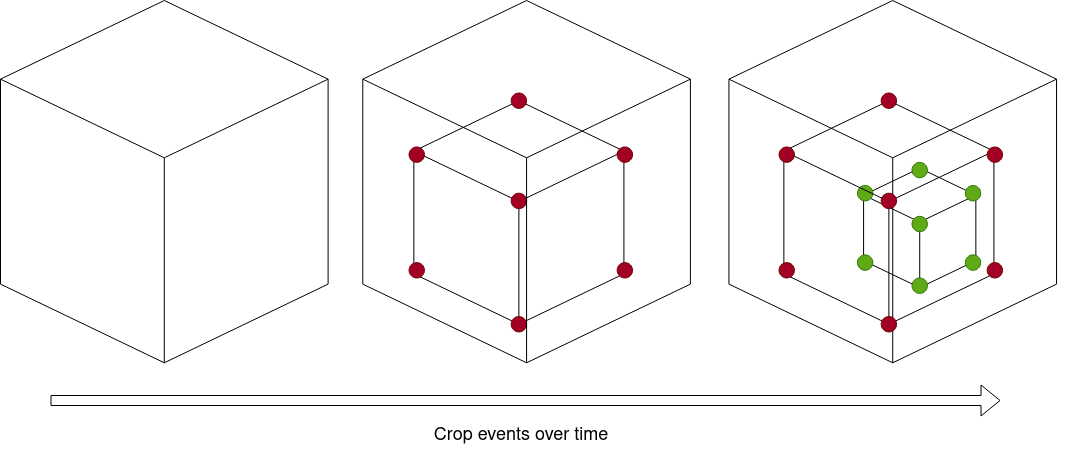
\includegraphics[width=0.6\linewidth]{figures/crop-cube.png}
    \caption{The relationship of the crop cube across cropping events to the full resolution data cube as the user drills down into a section of interest. The cropped sections refer to the marked red and green squares in the diagram; these sections are a selection made during a crop action. They are the portion of the data used to create the visualisation in the front-end services.}
    \label{fig:crop-cube}
\end{figure*}

% Virtual Reality Environment
% As the popularity of VR has boomed in recent times, there have been major developments in VR technology, driven by the demand for VR devices in the entertainment industry ~\cite{Farr2009}. 
% The virtual reality component of the front-end is embedded in the web browser application, and with packages like Three.js and WebXR, VR and three-dimensional environments can be embedded into web pages. 
WebXR grants access to the display of the headset, as well as the positions of the camera and controllers, allowing for integration with the web. 
Three.js was used to create the assets within the VR environment, such as the data cube used to display the astronomy data, and the UI elements which use canvases as textures to display text on a plane. 
These elements are made interactive through WebXR functions. 
The combination of these libraries facilitates a VR experience through the internet.
The data visualisation is presented within the VR space as a cube mesh with a three-dimensional texture used to map the three-dimensional data. 
This presentation method was selected because of its minimal processing cost~\cite{Ferrand2018}.
% choice to use volume rendering
%   present the data as is with minimal processing
%   iso-surface models must be generated using the raw data

% performs the rendering of the data
The data visualised by VRDAVis is volumetric astronomy data; however, this system would be able to visualise any volumetric data as long as it is in the HDF5 file format.
The HDF5 schema used is the same schema used by the fits2idia repository~\cite{fits2idia}, which is used to convert FITS files into the HDF5 files.
The mipmaps in the HDF5 file are stored according to their downsampling ratios.
For example XY\_2\_Z\_4 means that the x and y axis have been downsampled to a size 2 times smaller than the original cube and the z axis has been downsampled 4 times smaller than the original cube. 
The data arrives at the front-end from the data server in a float array format, where it is placed in a three-dimensional texture and rendered using a ray-cast shading technique.
The process of the ray-casting shader has the following steps:
\begin{enumerate}
  \item A ray is cast until it hits a bounding box of the volume texture.
  \item The ray takes a step through the volume and samples a point from the three-dimensional texture.
  \item The values that the ray sampled are added to an accumulator to determine the opacity of the pixel.
  \item The shader keeps track of the maximum value the ray has sampled.
  \item The ray continues to sample points until it has reached its maximum step count or the accumulated opacity reaches a 100\%.
  \item The shader then samples a two-dimensional colour map texture to retrieve a colour value for the pixel.
  \item If the opacity of the pixel is 0\%, the point is discarded.
\end{enumerate}

The rendering of the data with a ray-casting shader was implemented with the Three.js framework~\cite{Danchilla2012}, it can be easily integrated with React.js, a cross-browser JavaScript library built on top of WebGL. 
It is used to create and animate three-dimensional computer three-dimensional graphics within web browsers.
Three.js is widely adopted, and benefits from an active community that offers robust support. 

The shader goes through these steps for every frame, for every pixel on the screen. % cite
This is the most computationally expensive step in the visualisation process. 
Although ray-cast shading is computationally expensive, it depicts the data in a way that closely matches its structure, as if it were a high-resolution three-dimensional scatter plot.

For the user to view the visualisation with the VR headset in a virtual environment, a package is require which makes the three-dimensional environment compatible with VR displays and controllers.
WebXR provides access to input data related to the pose information from the headset and controllers, and output, which is the display within the headset. 
This technology enables web browsers to facilitate Virtual Reality (VR) and Augmented Reality (AR) experiences over the internet. 
It encompasses functionalities commonly associated with VR and AR devices.

In VRDAVis, WebXR is used to integrate an embedded VR environment into the client web application. It works in conjunction with Three.js and React.js to create an immersive three-dimensional environment, constituting the VRDAVis front-end application.

\subsubsection{User Workflow}

\begin{figure*}
    \centering
    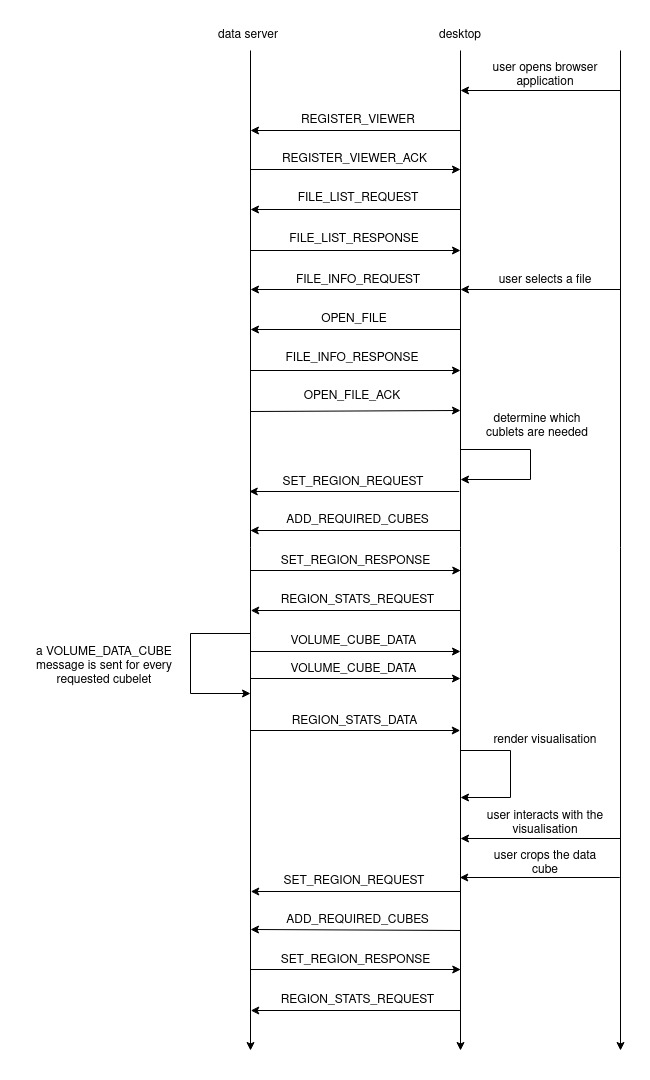
\includegraphics[width=0.6\linewidth]{figures/user-worklow(4).jpg}
    \caption{ A sequence diagram showing the user's interaction with an instance of the client application and the corresponding protocol buffer messages which are sent from the front-end to the back-end, as well as the responses from the back-end to the front-end. It shows the message sequence of the user opening the front-end application, selecting a file from a list, and cropping the visualisation.
    }
    \label{fig:user-workflow}
\end{figure*}

The user first opens an instance of the browser application on their desktop computer. 
When it is launched, this application instance creates a connection with the remote services such as the data and signalling servers. 
The signalling server connects the desktop client instance and pairs with the standalone VR headset if it is also connected to the signalling server at that time. 
This connection is made automatically once both devices are connected to the server. 
If the desktop device is not paired, then the user can pair it with an available unpaired device. 
When this peer-to-peer connection is created, the state of the visualisation can be transferred between the paired devices. 
The data server acknowledges the client application's connection, and the client requests a list of the available files on the server.

\begin{figure}
    \centering
    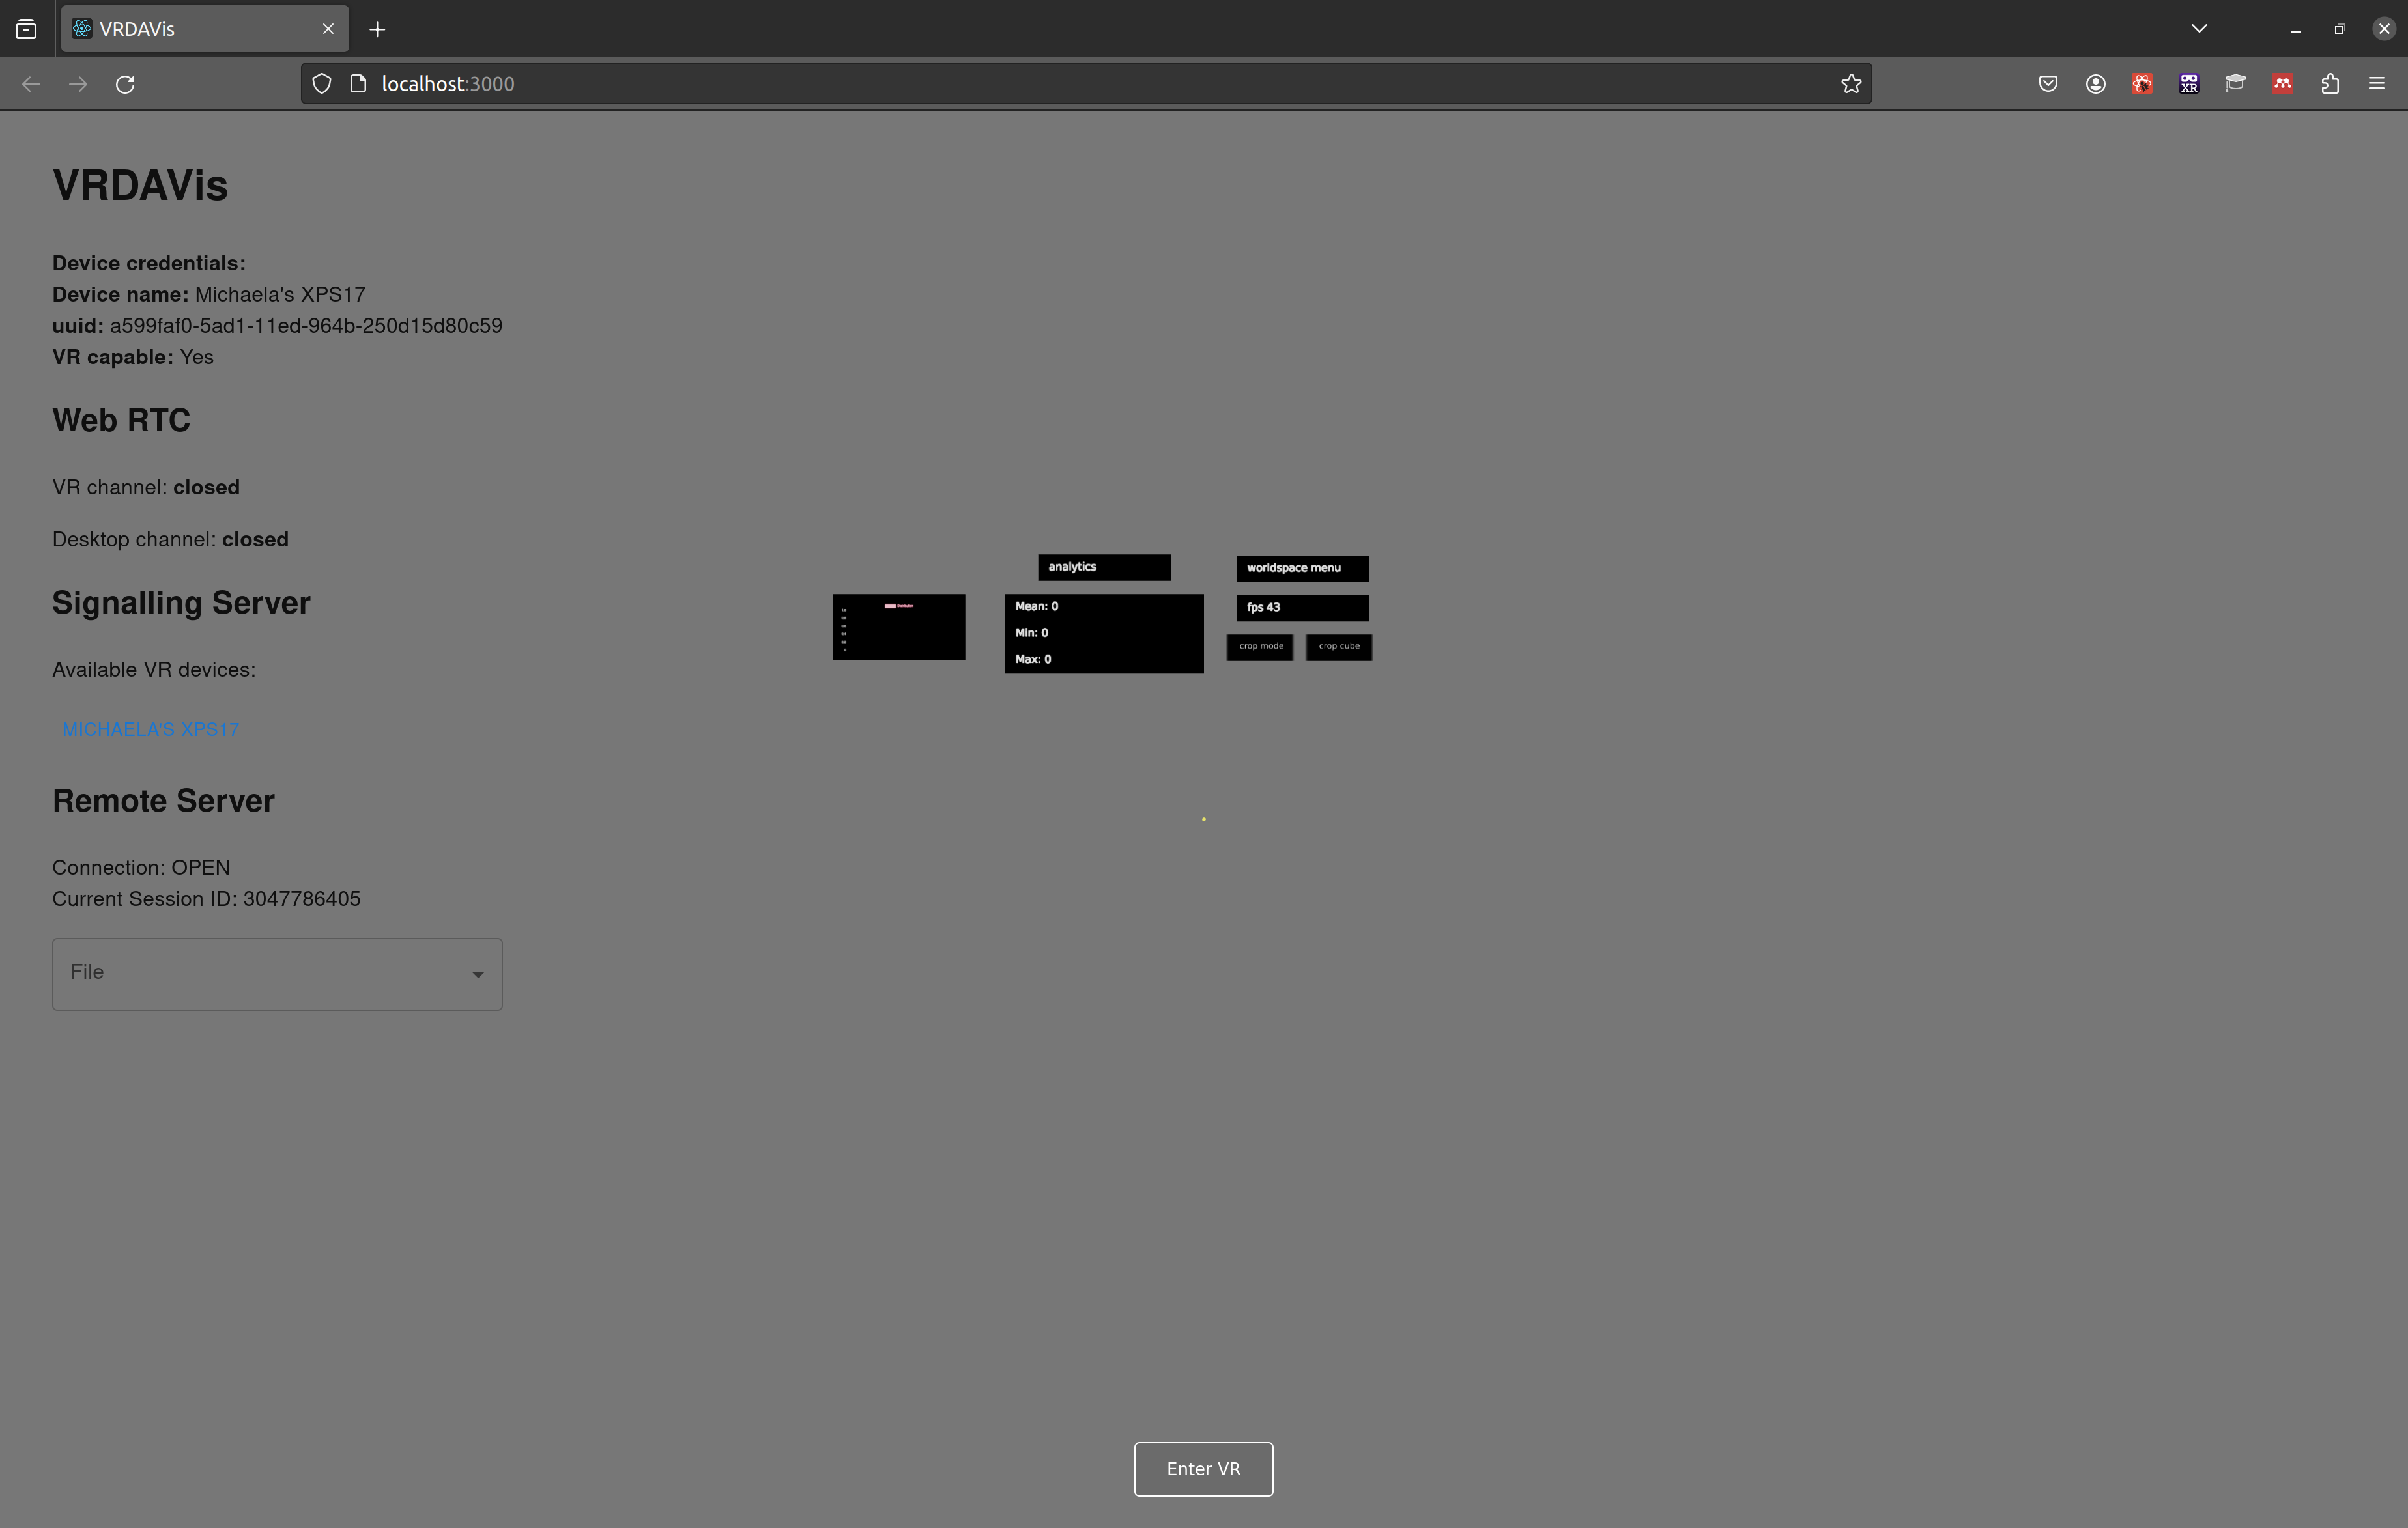
\includegraphics[width=\linewidth]{figures/screenshots/1.png}
    \caption{The appearance of the VRDAVis application when it is fist opened in the browser. In this instance the browser is Firefox. Some information about the current session can be seen on the left side of the screen, as well as the status of the peer-to-peer connection under the Web RTC heading, the available VR devices which can be paired with under the Signalling Server heading, and a drop down menu for selecting a data cubes under the Remote Server heading. Some VR environment assets can be seen in the centre of the screen.}
    \label{fig:screenshot-1}
\end{figure}

\begin{figure}
    \centering
    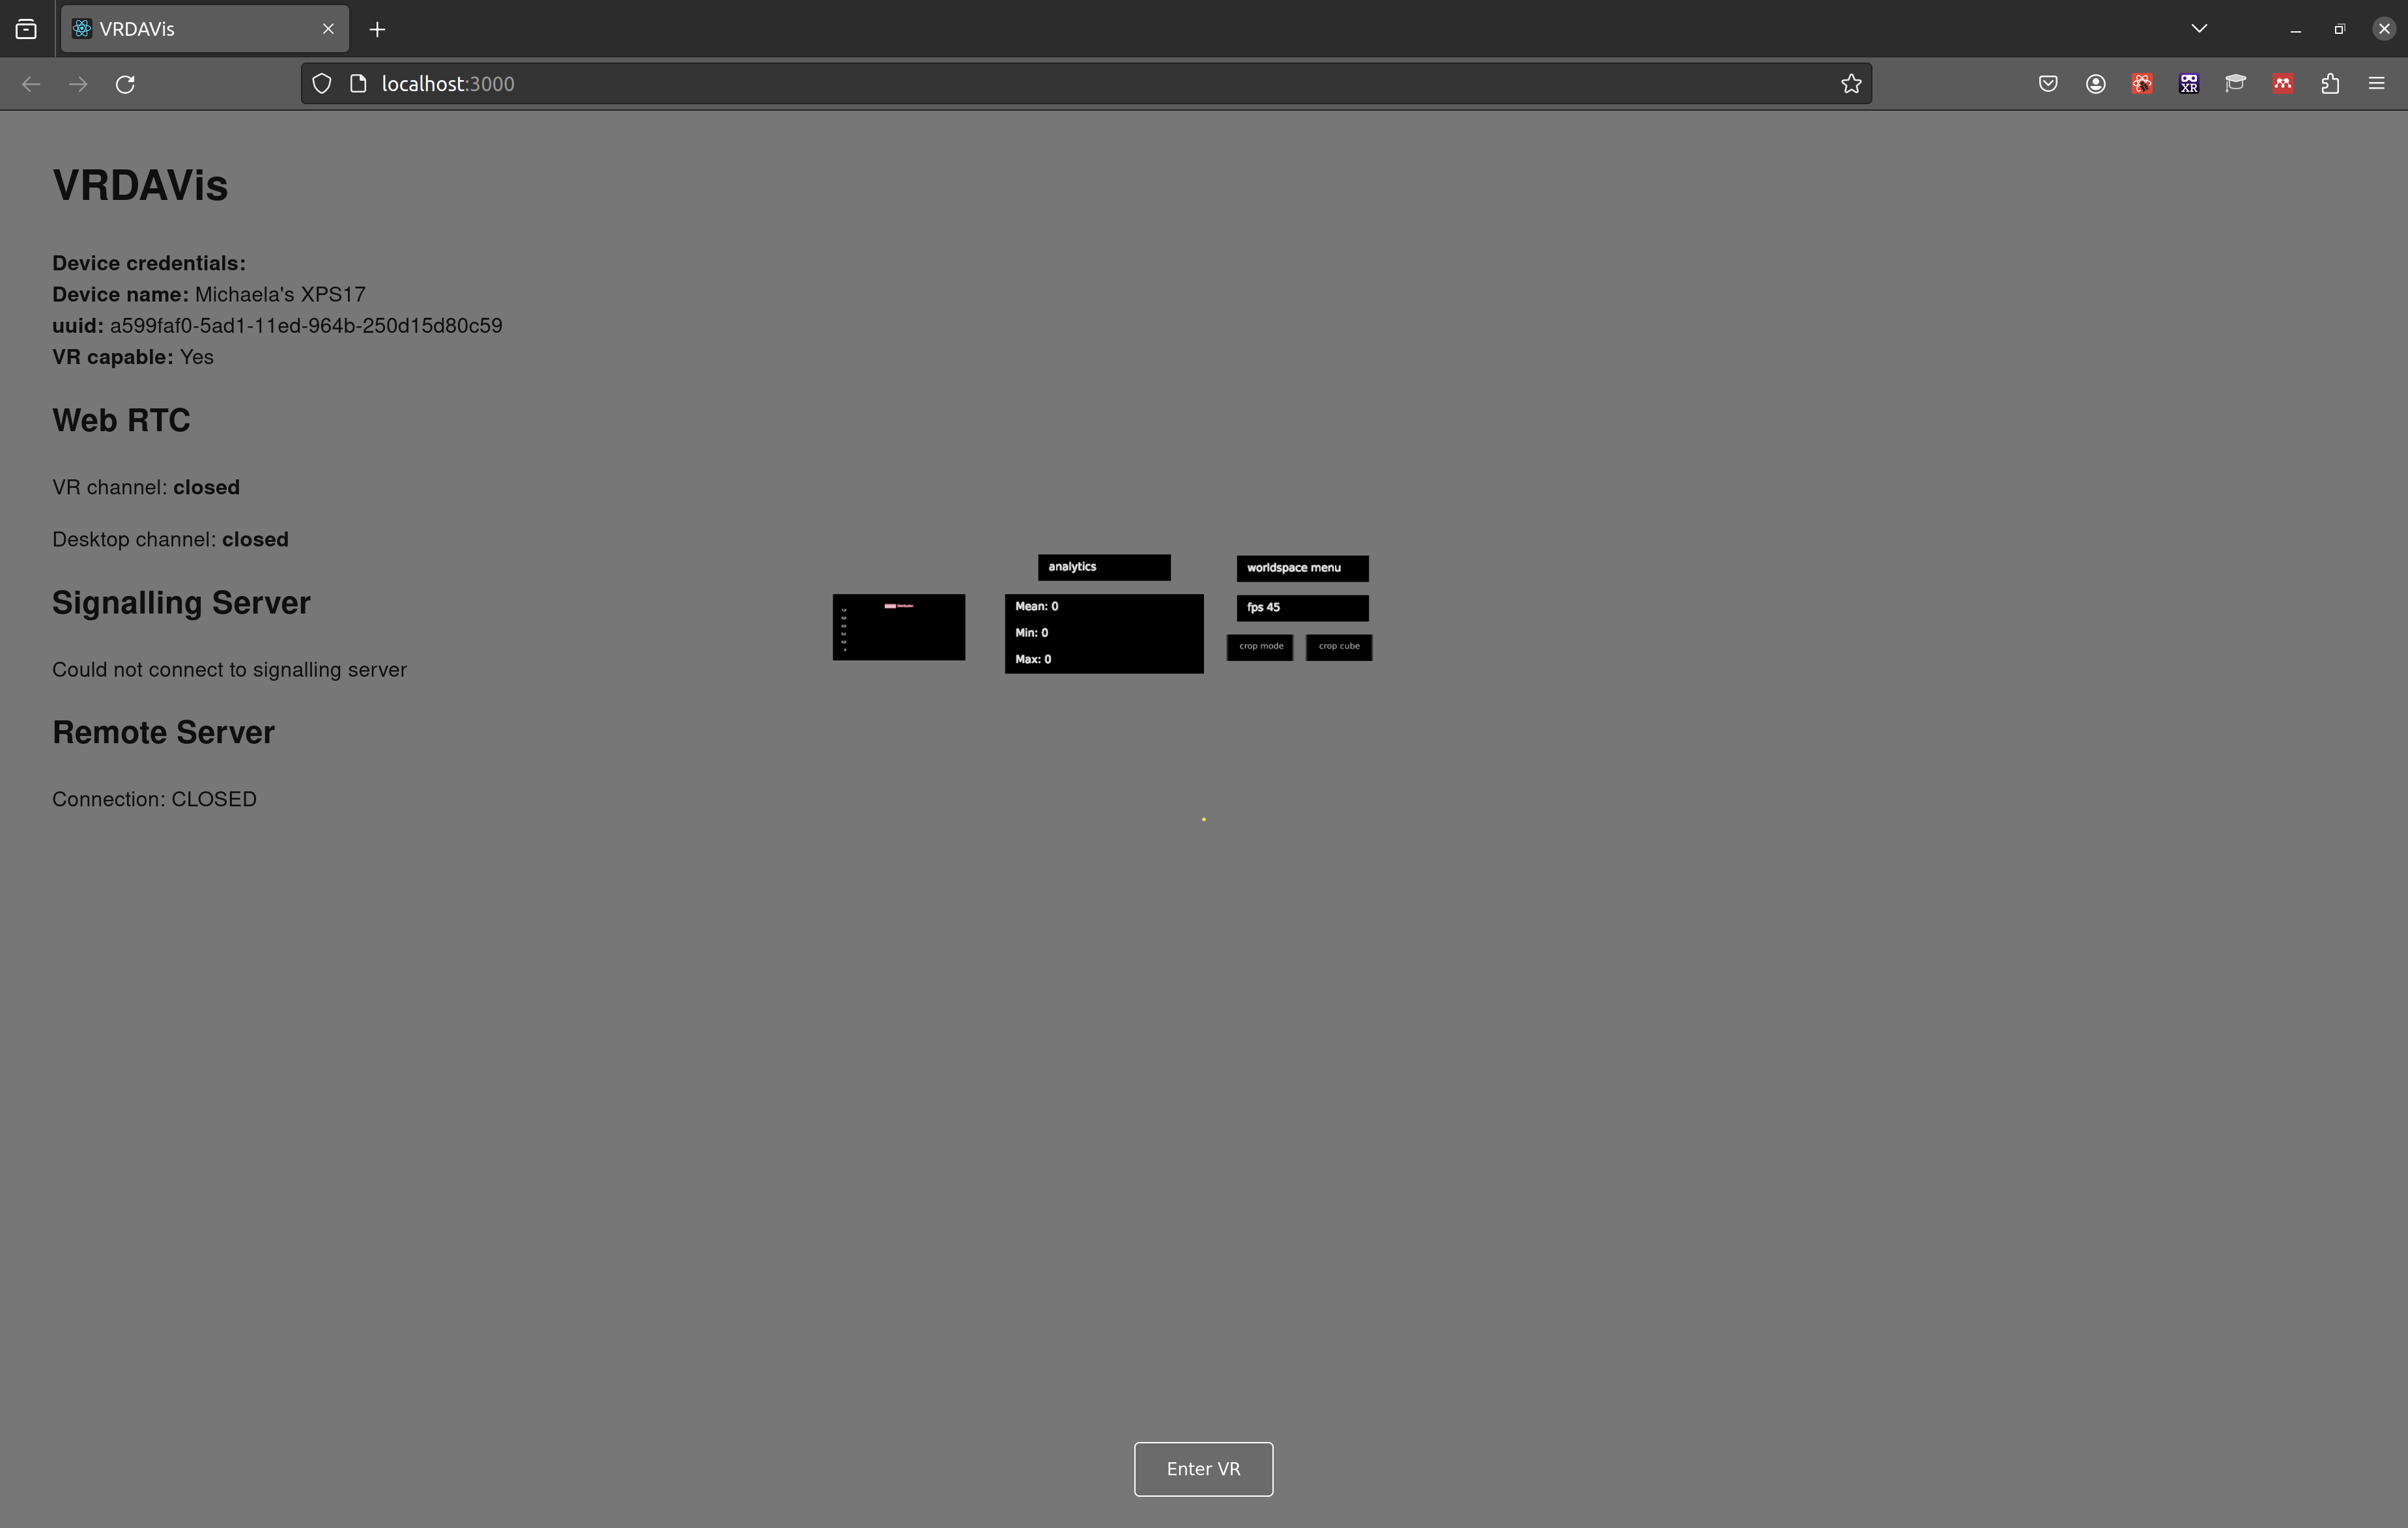
\includegraphics[width=\linewidth]{figures/screenshots/4.png}
    \caption{The appearance of the browser application when none of the remote services are available; there is no peer-to-peer connection, no connection to the signalling server, and no connection to the remote server.}
    \label{fig:screenshot-4}
\end{figure}

The data server sends the file list, and the user can choose which file they would like to explore. 
The user's file choice is sent to the data server, and the data server sends back some information pertaining to the selected file, such as dimensions and the size of the file. 
The client determines which cubelets it requires to generate the initial visualisation and requests them from the data server, while also specifying which analytics the data server needs to compute using the full-resolution data. 
The data server opens the file, reads the cubelets the client requested, compresses these cubelets into individual messages, and sends them to the client. 
Once the analytics are computed, they are also sent to the client.

When a cubelet reaches the client, it is decompressed and loaded into the GPU cache. 
The cubelet is then added to the three-dimensional, one at a time, until all the cubelets have been received and added. 
This three-dimensional texture is then rendered by the ray-casting shader.

\begin{figure}
    \centering
    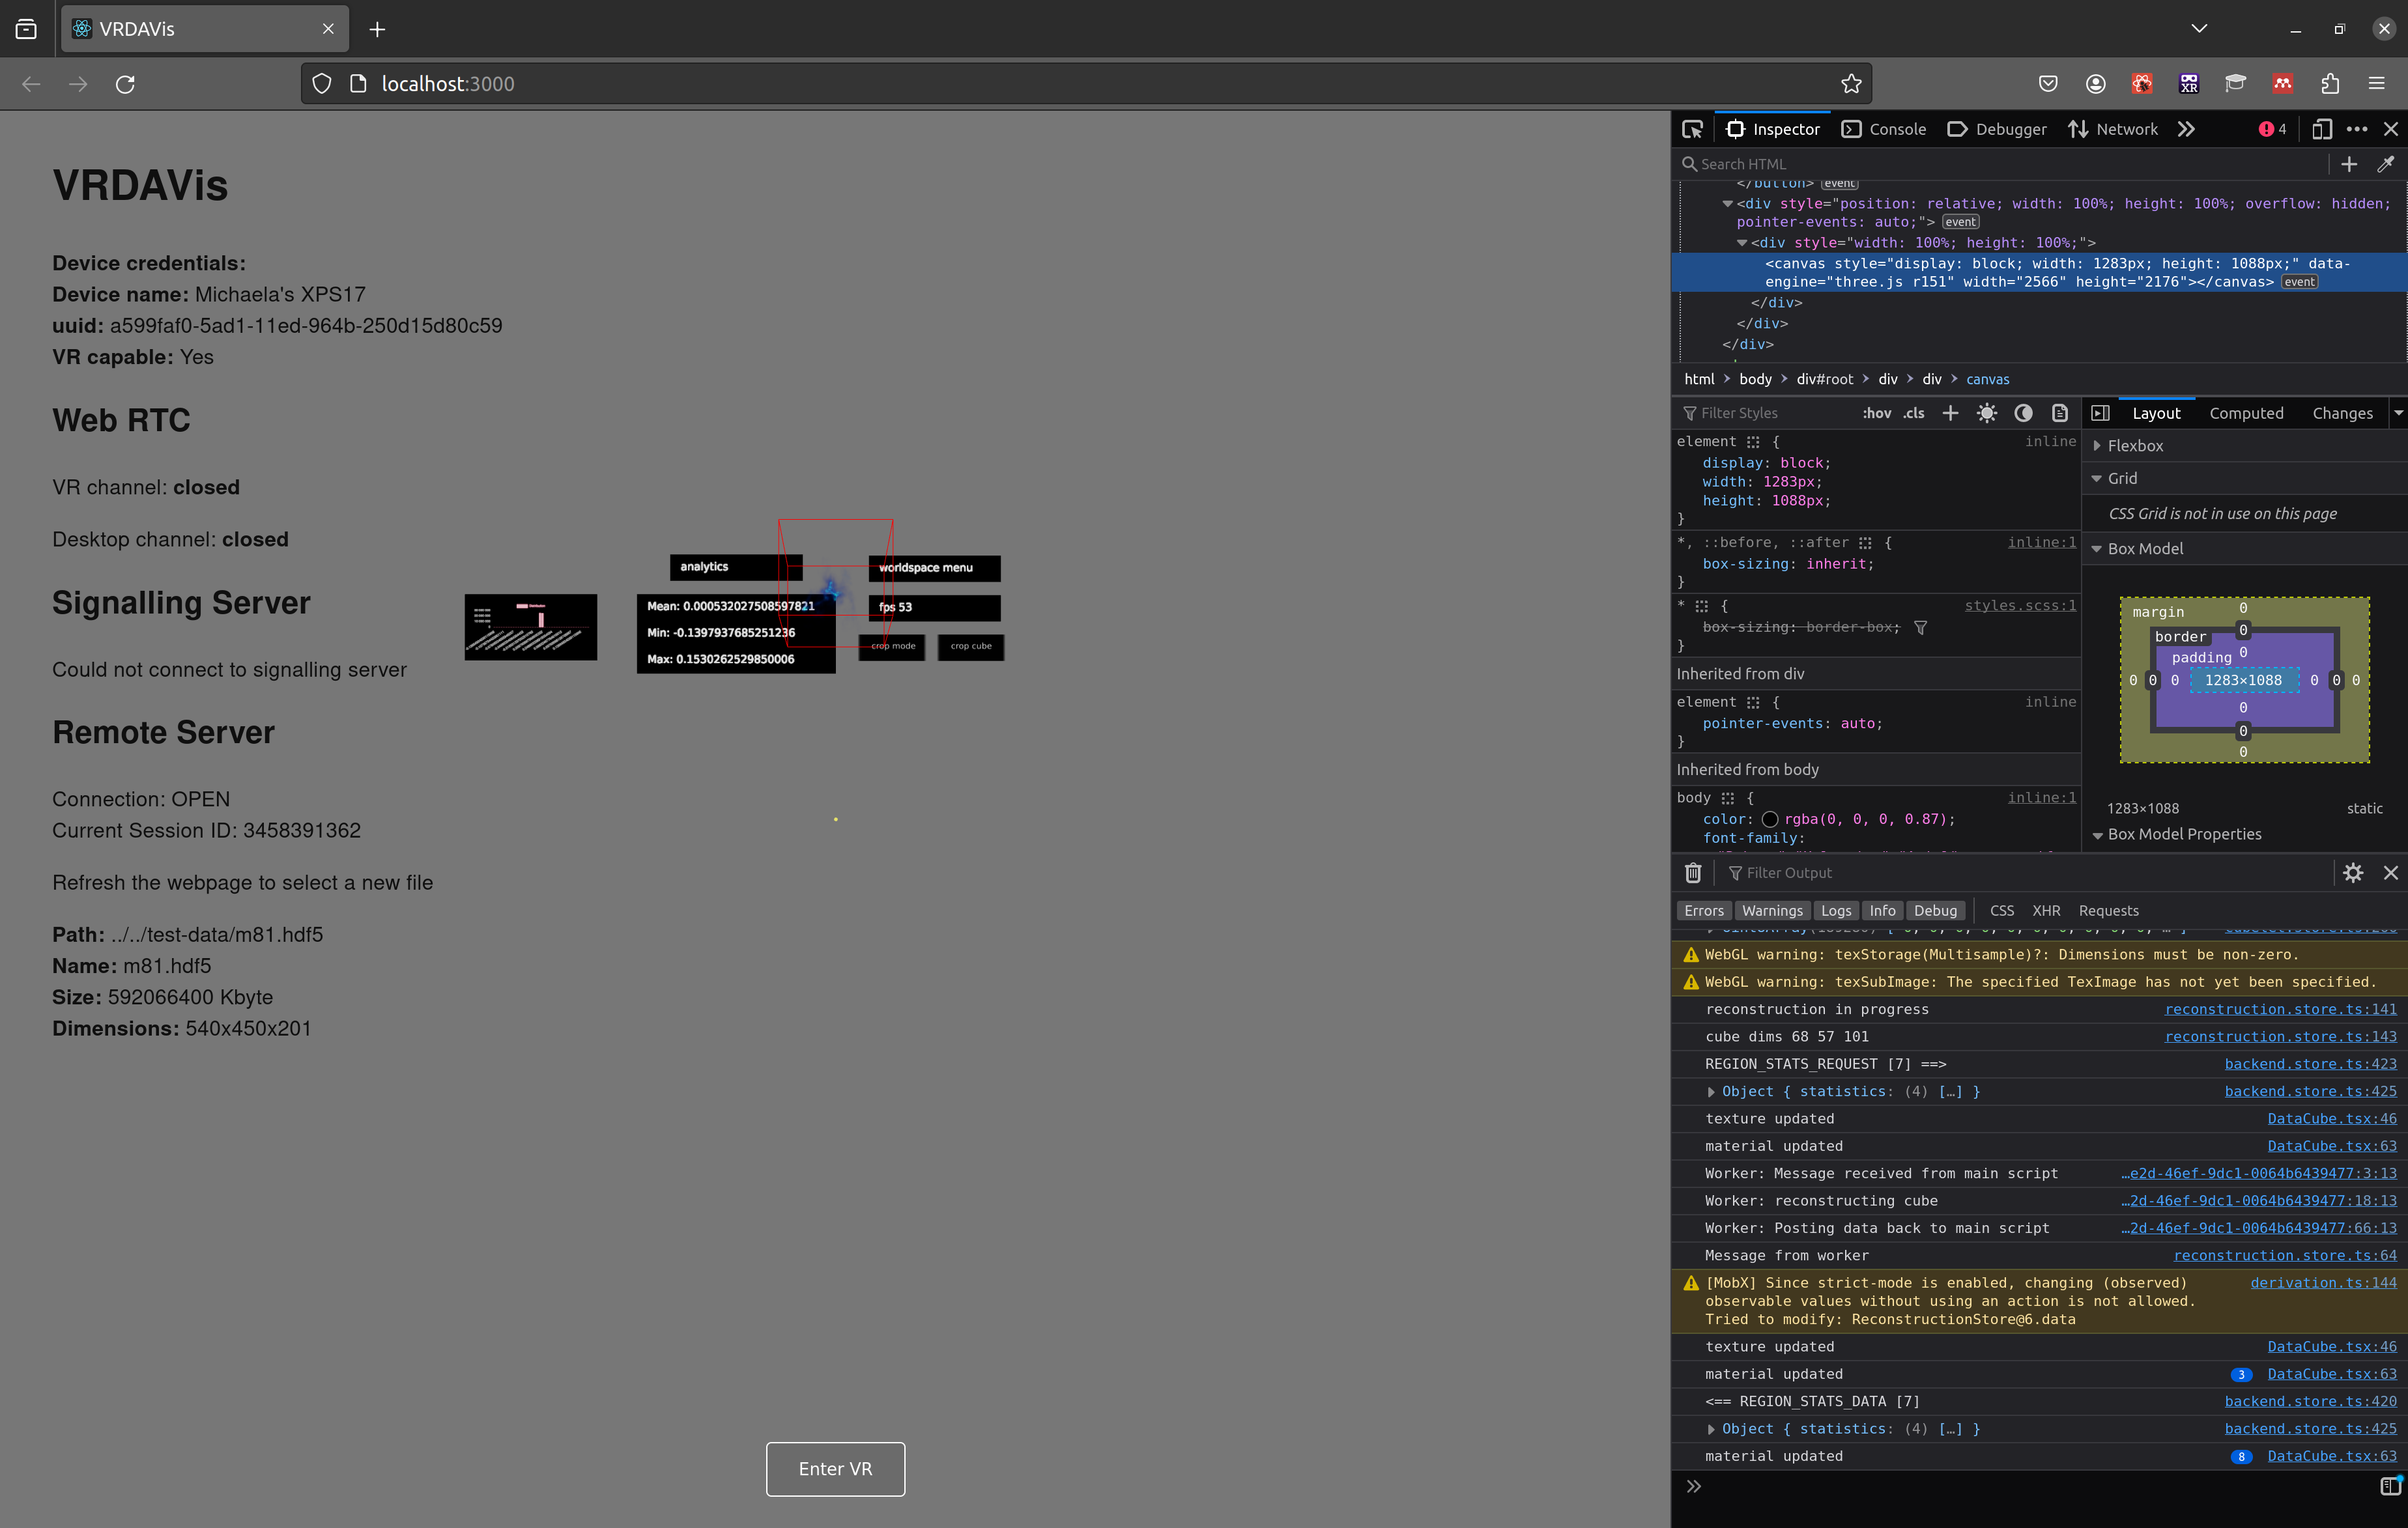
\includegraphics[width=\linewidth]{figures/screenshots/5.png}
    \caption{The view of the web browser application when a file has been selected and an initial visualisation of the data cube is within the VR environment. Some additional information about the data cube is displayed under the Remote Server heading; the path of the file on the remote server, the name of the file, the size in kilobytes, and the dimensions of the data cube.}
    \label{fig:screenshot-5}
\end{figure}

The user can then choose to switch to viewing the visualisation on the standalone VR headset. 
If the user switches to the headset, all the state information is sent over the peer-to-peer connection. 

The headset client uses the state information to start its own session on the data server and request the same cubelets as on the desktop client instance. 
The VR instance does not need the desktop instance to function; the user can choose to start the entire visualisation process on the VR headset by starting the client browser application on the browser. 
The main difference between the instance of the application on the desktop and the VR headset is that the VR headset client instance has the entry point to the VR environment, whereas the desktop does not have the capabilities to view a VR environment.

When the user enters the VR environment, they can interact with the visualisation in a three-dimensional space and view the analytics of the data. 
\begin{figure}
    \centering
    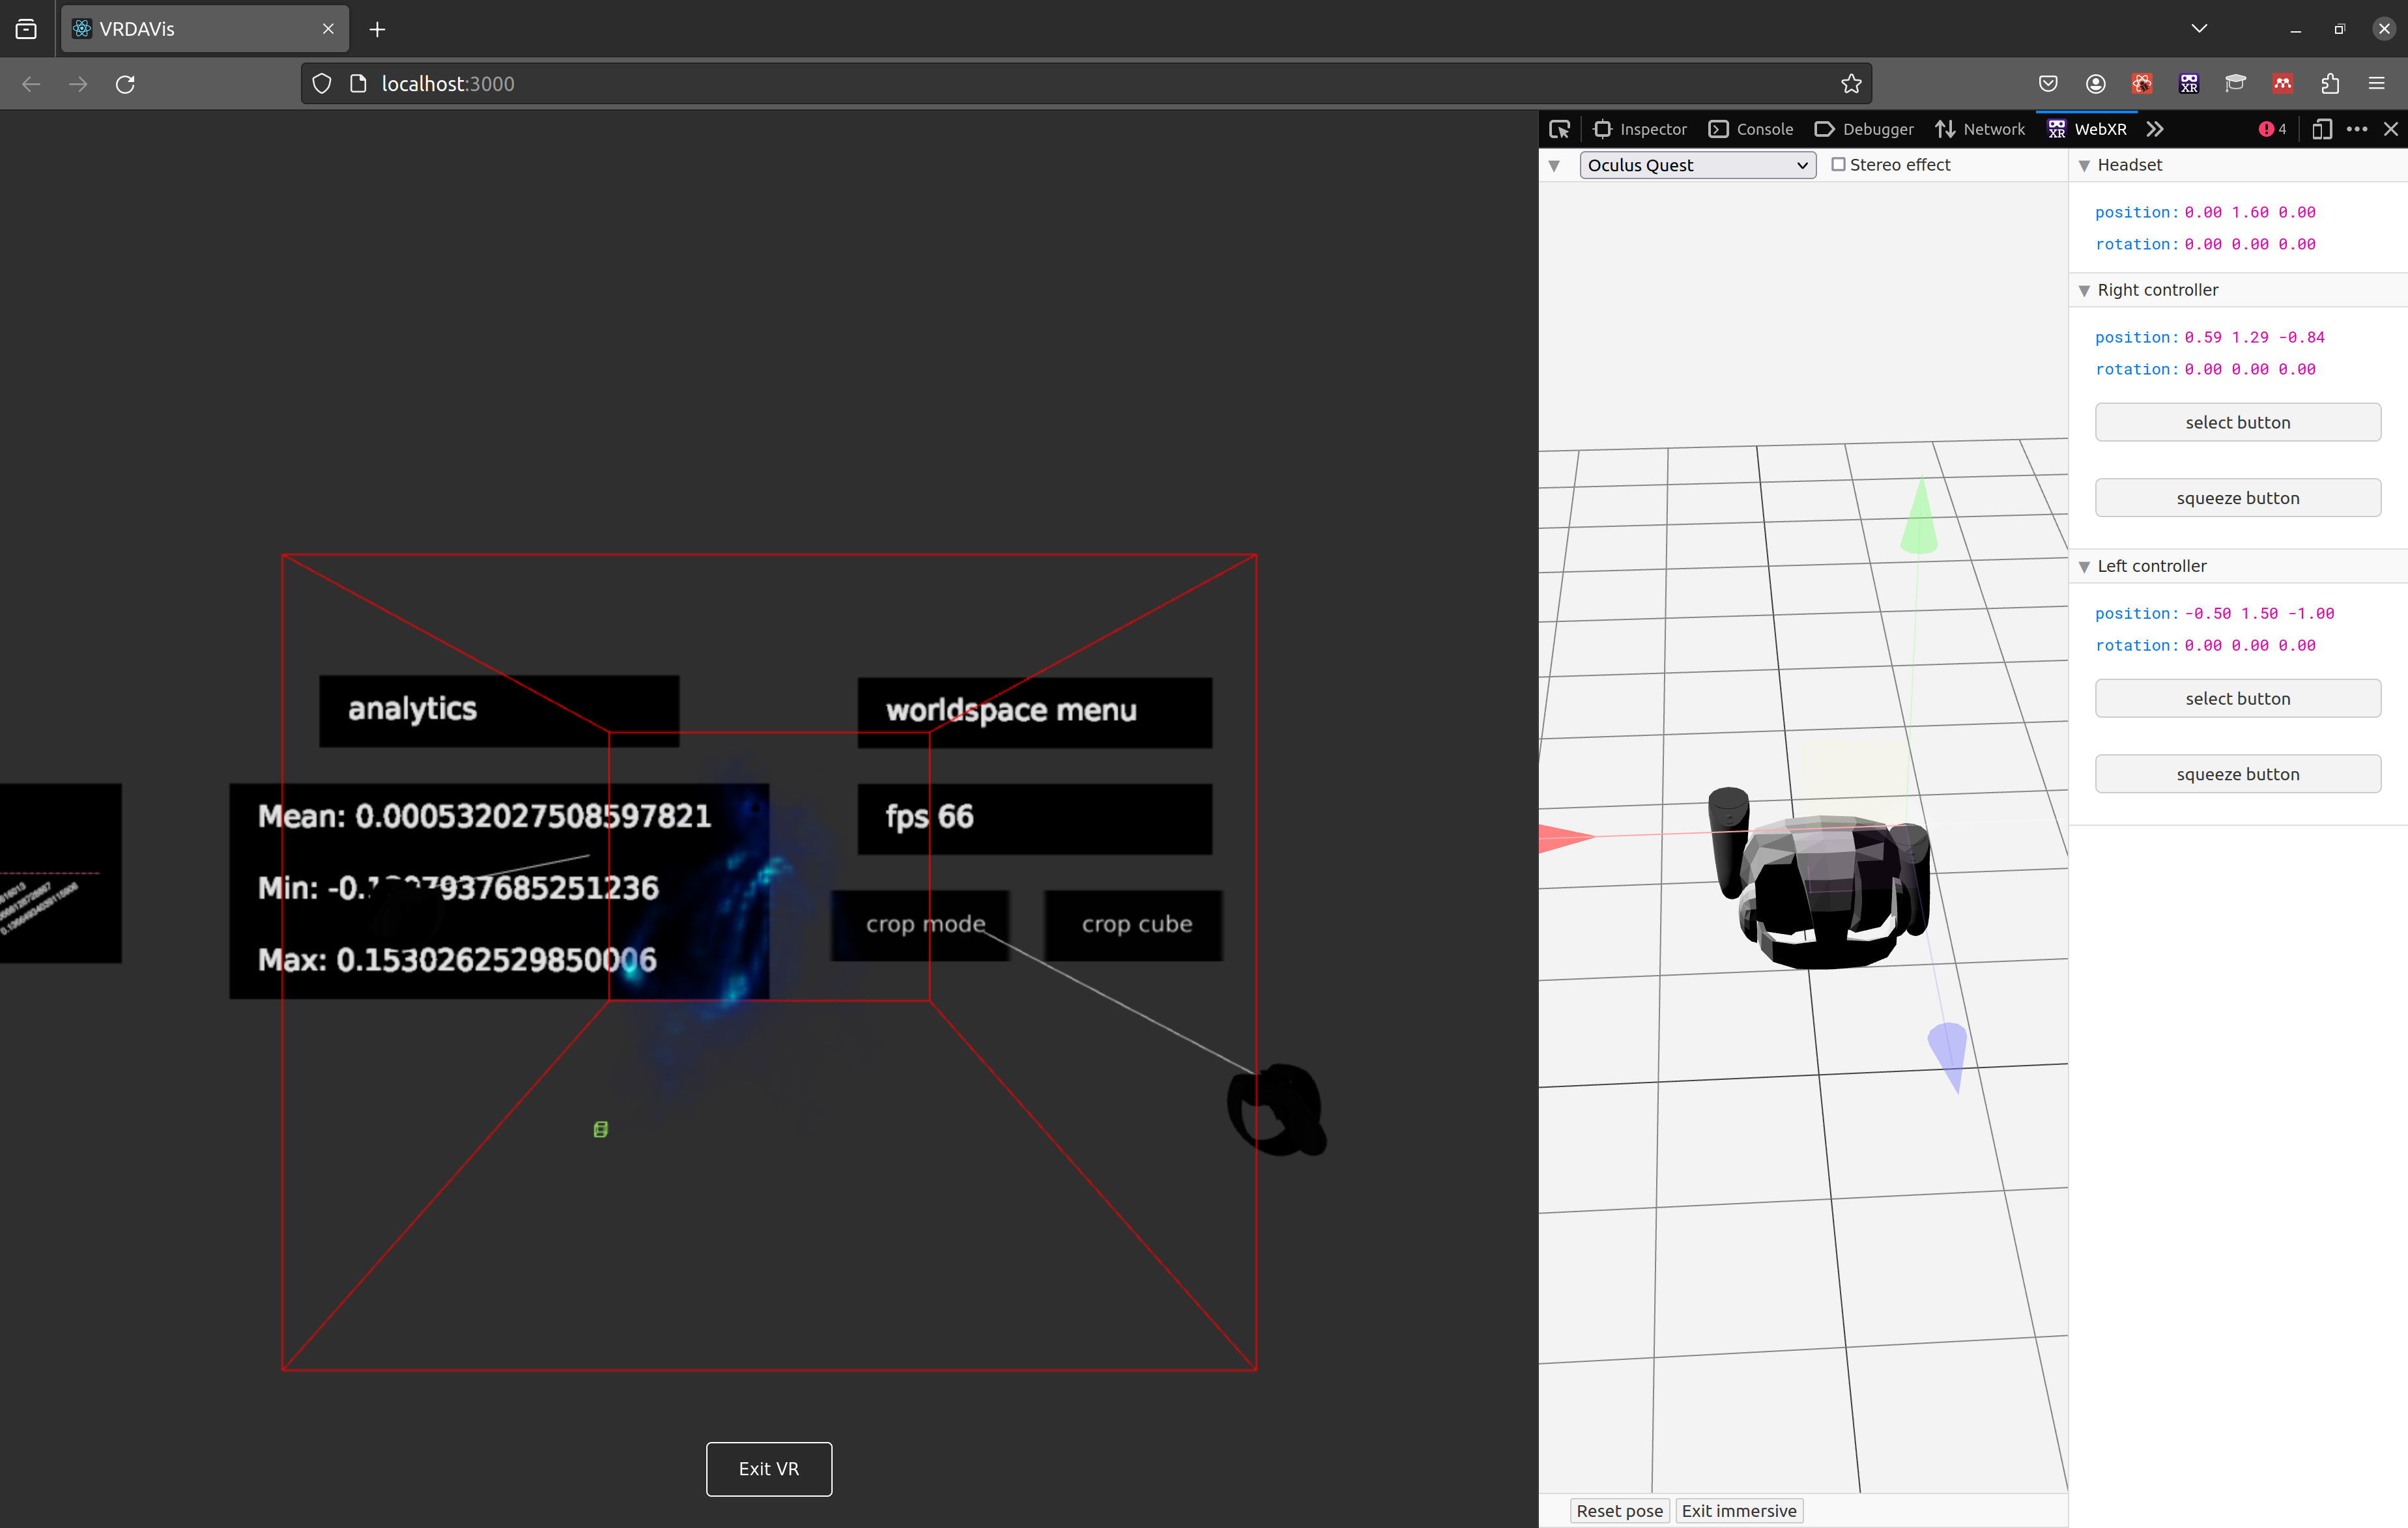
\includegraphics[width=\linewidth]{figures/screenshots/9.png}
    \caption{The view from inside the VR environment. The assets which could be seen on the centre of the view are now tangible within the VR environment. The data-cube is now a three-dimensional object and the analytics menu can be seen behind it. The WebXR browser plugin is used to view the VR environment from the browser window on a conventional screen. The plugin interface is displayed on the right side of the browser window.}
    \label{fig:screenshot-9}
\end{figure}
The user can crop the visualisation to get a higher-resolution version of the data by using the crop function; the user drags a box over the section they would like to take a closer look at and then selects the crop button. 
The client application determines which resolution level is appropriate for cubelet selection and sends a list of cubelets to the data server. 
The server fetches the cubelets and computes the analytics in the same way as it did for the initial visualisation. 
This process happens every time the cube is cropped until it reaches the highest resolution level, which is the full-resolution data. 
The size of the cubelets is determined by predetermined, internal values in the remote and front-end services.

\begin{figure}
    \centering
    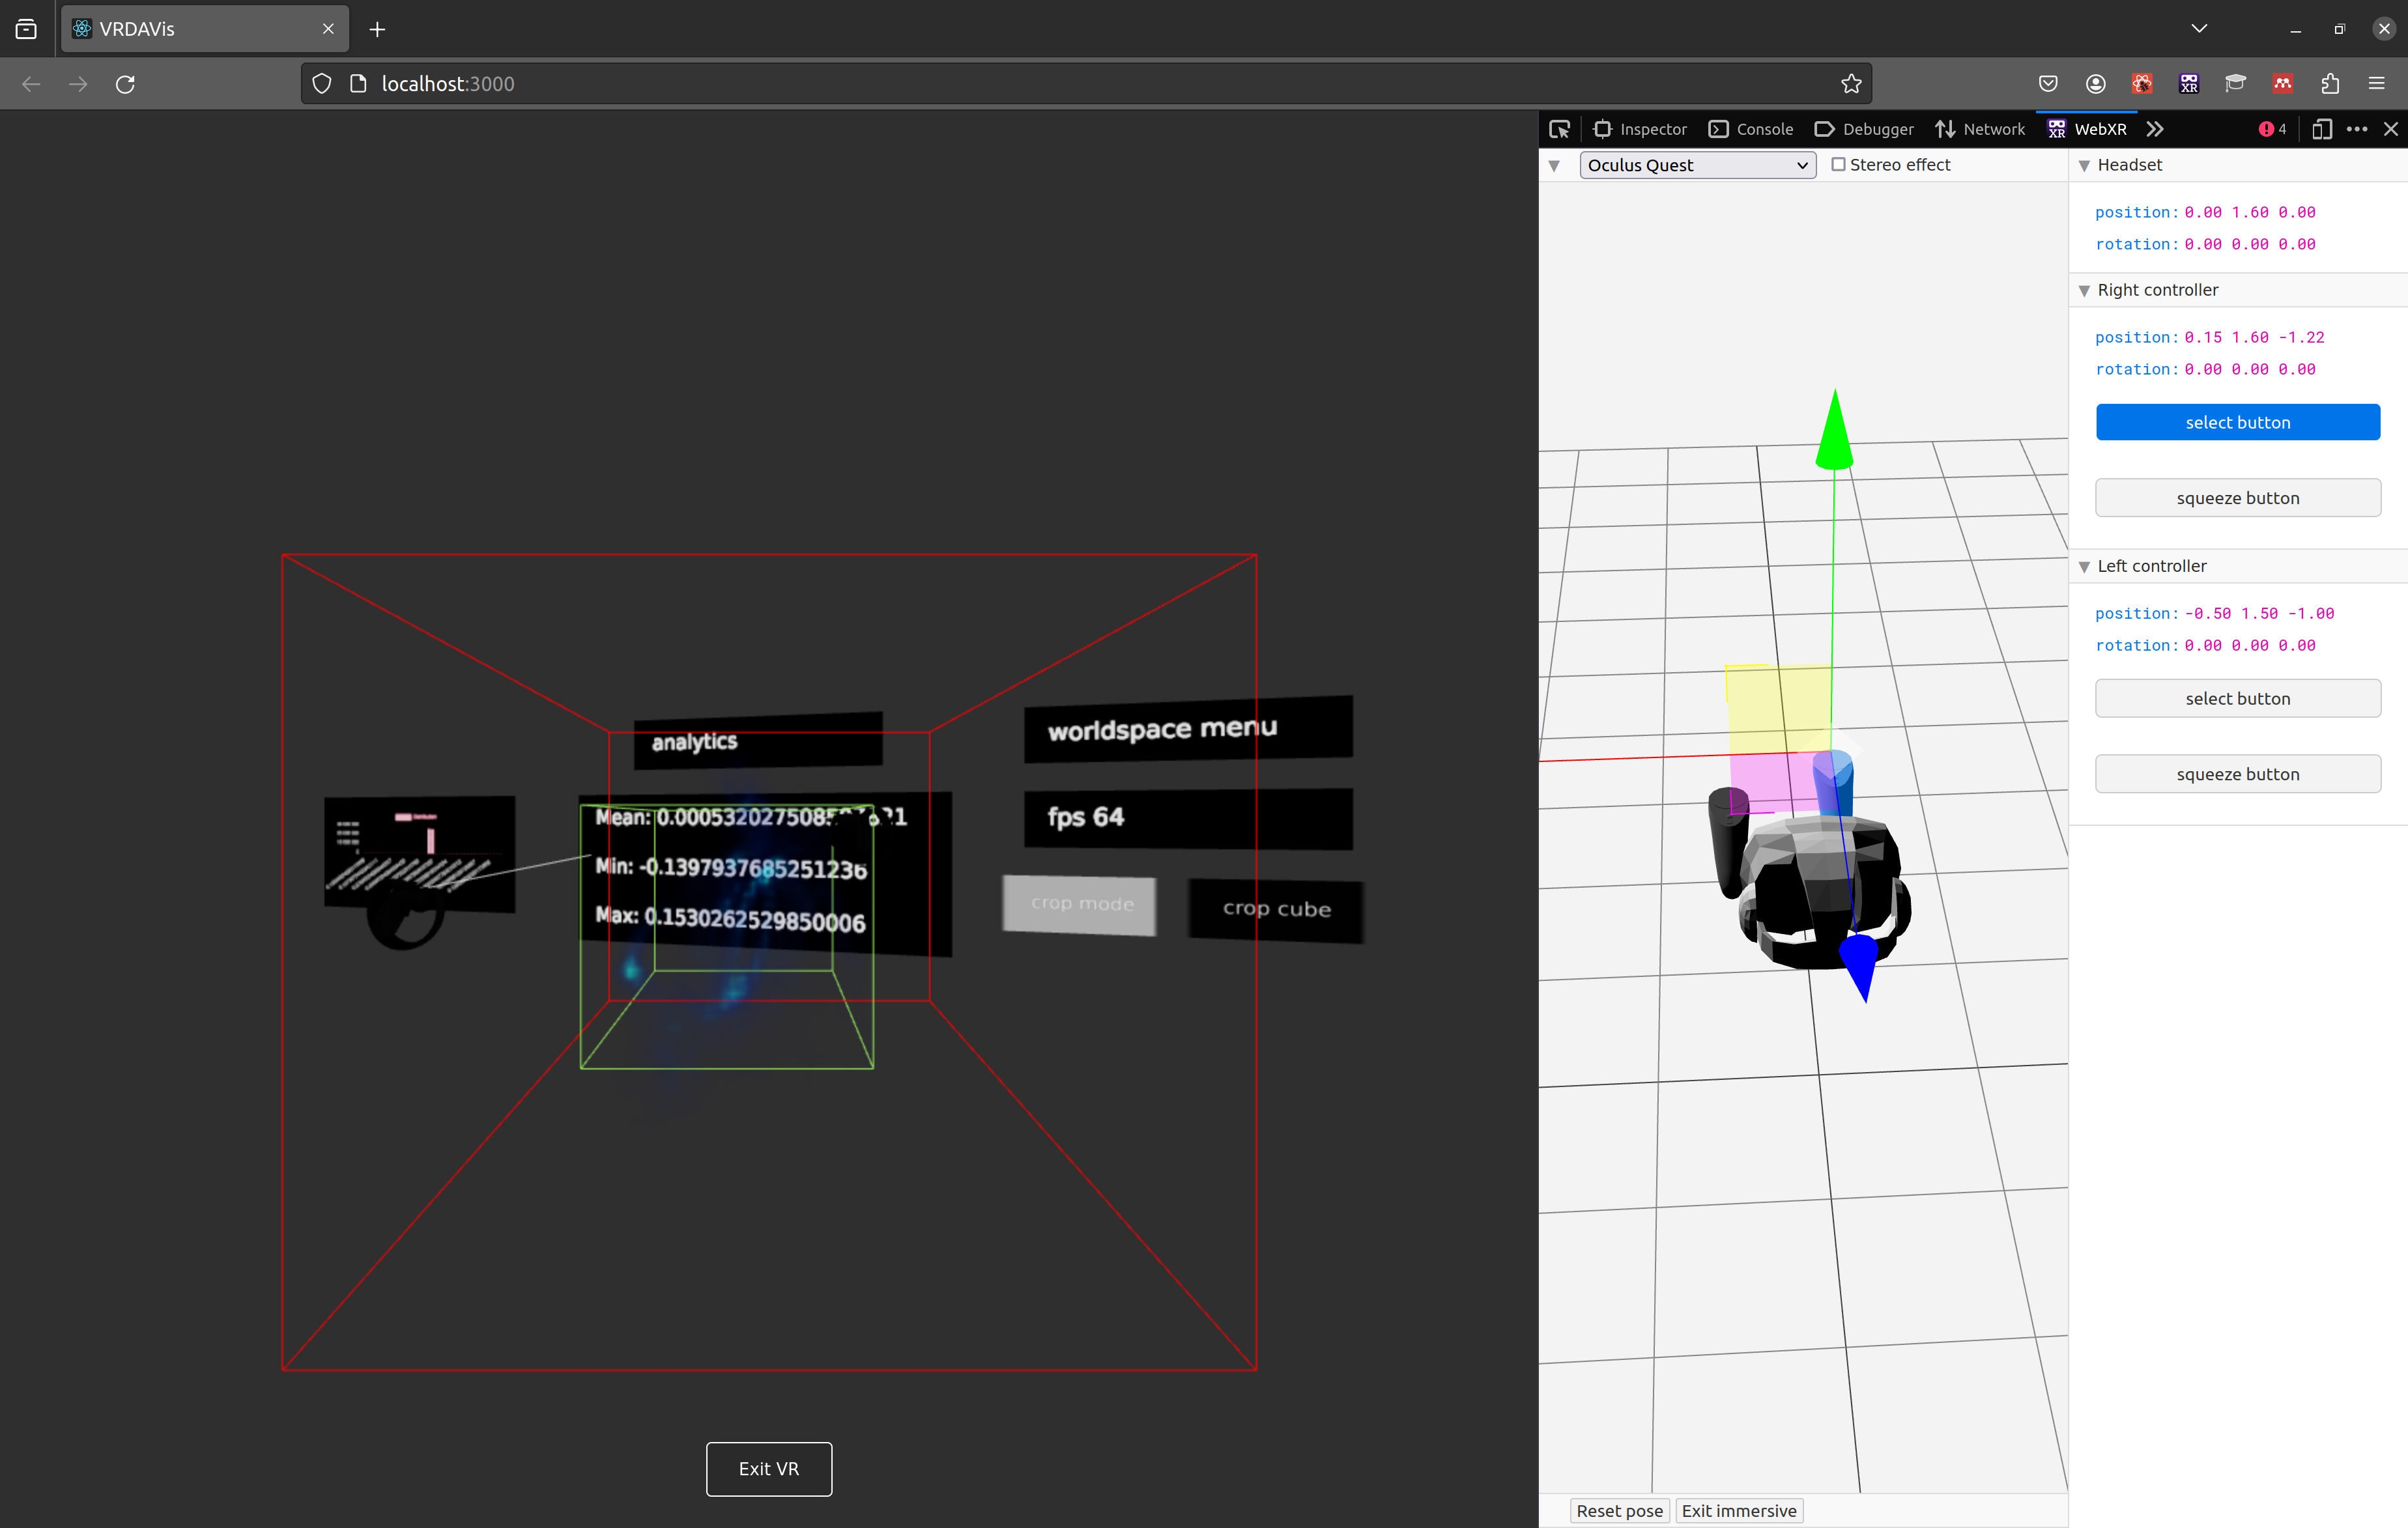
\includegraphics[width=\linewidth]{figures/screenshots/10.png}
    \caption{An example of a data cube displayed in the VR environment. The red cube represents an area within full dimensions of the data cube, and the green cube shows the selected crop area.}
    \label{fig:screenshot-10}
\end{figure}

\newpage
\section{Initial Evaluation}
\label{sec:initial-evaluation}

% have industry experts review the system and log their feedback to come to a conclusion

% intro
%   explain scope
%   this evaluation is designed to judge the sentiment of industry experts
%   open a line of communication with potential users 
%   receive feedback and guidence on future improvements
%   the system is optimised for user experience on the standalone VR headset, therefore, their feedback is crucial
%   semi-structured interviews guides the participants through their interactions with VRDAVis and allow them to progress at their own pace
%   some questions will be asked once they are finished with their evaluations
The evaluation was designed to judge the sentiment of expert users and open a line of communication to receive feedback and guidance on future improvements. 
These expert users were individuals who are researchers in the astronomy field; they also required some experience with VR and experience of using a similar system such as i-Davie. 
They are aware of the requirements of a successful VR experience, as well as a successful astronomy data visualiser.
VRDAVis is an experimental system and has some shortcomings that may confuse a novice user. 
The VRDAVis system is optimised for user experience on the standalone VR headset, which makes their feedback crucial. 
Semi-structured interviews guided the participants through their interactions with VRDAVis, allowing them to progress at their own pace. 
Additionally, some questions were asked once they had finished their evaluations to further refine the system based on their insights and experiences.

% methodology
% the design of the experiment
%   the user will be asked to use the system from starting from the laptop and themoving to the vr headset
%   the user will be asked to complete tasks such as
%       select a file to view on the laptop
%       transfer the state to the VR headset
%       enter the VR environment via the VR headset
%       manipulate the visualiasation of the file
%           this invloves translating, rotating, and scaling the visualisation
%       crop the visualisation 
%   all the participants use the same system
In the experiment, the participant will be asked to start using the system on a laptop and then move to the VR headset. 
The participant will be required to complete tasks such as selecting a file to view on the laptop, transferring the state to the VR headset, entering the VR environment via the VR headset, and manipulating the visualisation of the file. 
This manipulation involves translating, rotating, and scaling the visualisation, as well as performing an action where the visualisation's resolution is scaled up as it is cropped. 
All participants will use the same system to ensure consistency in the experiment.

\subsection{Participants}
% participants
%   the participants were pre selected from member if the Instituite of Data-intensive astronomy
%   all paticipants are briefed on tasks they will perform as well as the protocol if they start feeling nauseous while using the VR headset, this is known as simulator sickness
%   they are all asked to sign a consent form belfore the comensment of the evaluation
%   the participants evaluating the VRDAVis system are industry experts in astronomy and computer science
%   these participants are also well versed in VR technology
%   they are regular users of VR interfaces
%   also have experience using VR systems designed to visualise astronomy data
%   such as i-Davie
%   VRDAVis is an experimental system and has some shortcomings which may confuse a novice user
%   having some experience in VR bolsers the user from becoming disorientated and ahelps them avoid simulator sickness
%   during the duration of the evaluation if a user does begin to experience simulator sickness the evaluation is stopped to tend to the participant
%   once the participants recovers from the simulator sickness they can their continue with the evaluation or they can stop the evaluation

The participants in the experiment were pre-selected from members of the Institute of Data-Intensive Astronomy. 
All participants were briefed on the tasks they would perform as well as the protocol to follow if they start feeling nauseous while using the VR headset.
% This phenomena is a condition known as simulator sickness, and is common occurrence in users not well acquainted with the sensations that occur while using a VR headset.
% No long term harm comes from this as the feelings of nausea pass once the VR headset is removed.
All participants were all asked to sign a consent form before the commencement of the evaluation. 
It reiterates the tasks they will performing and what data will be collected during the experiment.

\subsection{System Set-up Description}
% System set-up description
%   a system used to visualise astronomy data cubes
%   a laptop and VR headset which communicate with remotes systems as well as each other
%  all for the purpose of visualisaing an astronomy data cube on laptop or VR headset
%   full description of the VRDAVis system can be found in the system design section
To conduct the evaluation, a carefully designed set-up is essential to ensure smooth transitions between the laptop and VR headset, as well as to capture the participants' interactions and feedback accurately. 
The environment is a quiet, controlled space free from external disturbances, equipped with chairs and adequate lighting. 
The equipment includes a laptop with the necessary software for viewing and manipulating the selected file, along with a standalone VR headset and the required controllers. 
Participants will begin by selecting and viewing the file on the laptop, then transition to the VR headset and interact with the visualisation.
These actions include translating, rotating, scaling, and cropping the visualisation. 
The procedure involves a briefing area where participants are informed about tasks and protocols, including handling simulator sickness, and sign consent forms. 
The task area houses the laptop, while a designated transition spot allows for easy movement to the spacious VR area. 
Monitoring and support are provided to the participants by the conductor of the experiment, who observes for signs of discomfort and offer immediate assistance, with video and audio recording equipment capturing interactions and feedback. 
Post-evaluation, participants relax in the briefing area where they discuss their experience and answer some questions from the conductor. 
Clear guidelines are in place for handling simulator sickness, including the option to stop and resume the evaluation. 
This set-up ensures a controlled, supportive environment, prioritising participant well-being and enabling the collection of detailed feedback on the VRDAVis system.

% metrics / questions
%   gather qualitative data about the user's experience
%       anything the user highlights during their time using the system
%   see which taks they struggle with the most
%   how well they interact with the user interface
%   what they think of seeing the data-cube visualised in three-dimensional space
%   what they think of interacting with the data-cube visualised in three-dimensional space
%   what they think of the workflow of the system
\subsection{Metrics}
During the evaluation, several metrics were collected to assess the VRDAVis system. 
Qualitative data about the user's experience was gathered, including any highlights or noteworthy comments they made while using the system. 
Observations were made to identify which tasks participants struggled with the most and how well they interacted with the user interface. 
Feedback was collected on their impressions of seeing the data cube visualised in three-dimensional space and their thoughts on interacting with it. 
Participants were asked for their opinions on the overall workflow of the system, providing valuable insights into its usability and effectiveness.

\newpage
\section{Evaluation Results}
\label{sec:evaluation-results}

% introduction
The goal of the evaluation was to gain insight and feedback from users regarding the VRDAVis system. 
Feedback was gathered by having users evaluate the VRDAVis system, and the results highlight both the successful parts and areas for improvement.

% PARTICIPANT 1 - ALEX
%   developer of i-Davie

% ### Feedback Summary

% #### Participant's Perspective on i-Davie vs. Current Software

% 1. **Visualization and Interactivity**
%    - **Strengths:**
%      - Standalone visualization is appreciated.
%      - Volumetric rendering on a standalone device is seen as a significant achievement.
%      - Performance is commendable; it runs smoothly without noticeable stutter.
%    - **Weaknesses:**
%      - Lack of interactivity: The participant finds the interactive elements, such as the selection box, not very intuitive
%      - Immersion: The 3D space does not feel immersive, partly due to the absence of a cursor to show point values and coordinates.
%      - Menu System: Menus feel awkward and are not optimised for VR, affecting usability.

% 2. **Comparison with i-Davie**
%    - **Differences:**
%      - i-Davie is praised for its interactivity, which is perceived as lacking in the current software.
%      - Selection mechanism: i-Davie allows for precise selection, which the current software does not replicate well.
%    - **Suggestions:**
%      - Implement real-time interaction features to show values and coordinates.
%      - Improve the selection mechanism to be more intuitive and precise.

% 3. **Menu and UI System**
%    - **Issues:**
%      - The current menu system feels off and not user-friendly.
%      - UI libraries are not designed specifically for VR, leading to performance trade-offs.
%    - **Suggestions:**
%      - Emulate familiar UI interactions from desktop environments (e.g., dragging menus by the top banner).
%      - Make UI elements more VR-friendly and responsive.

% 4. **Workflow Integration**
%    - **Process:**
%      - Participants prefer starting with the desktop to select files and then transitioning to VR for 3D visualisation.
%      - Direct file selection in VR is less preferred due to occasional need for quick adjustments.
%    - **Feedback:**
%      - Integration is seen as more of a workflow endpoint rather than a seamless process.
%      - Lack of productivity features: Users need a way to export or record data from VR sessions effectively.
%    - **Suggestions:**
%      - Enhance the workflow by enabling productive output from VR sessions.
%      - Ensure straightforward crash recovery to prevent workflow disruptions.

% #### Interviewer's Response

% - **Acknowledgment:**
%   - Recognised the feedback about interactivity, menu usability, and workflow integration.
%   - Acknowledged the limitations due to the current UI library and its performance impact.
% - **Future Improvements:**
%   - Plans to address interactive elements and menu usability in subsequent updates.
%   - Intends to focus on polishing and adding necessary features based on the feedback received.

Participant 1 noted a positive experience with the visual quality and interactive aspects of VRDAVis, specifically praising the ease of use for cropping and analysing different data segments. 
They highlighted the significance of having an immersive experience for visualising complex data, which they found to be more intuitive compared to traditional two-dimensional methods. 
However, they mentioned the importance of improving the system’s stability, as they experienced some technical glitches. 
They also suggested that additional features, such as more sophisticated data manipulation tools and enhanced resolution, could further enhance the usability and effectiveness of VRDAVis. 

% leave out immediate summaries
% The feedback highlights key areas for improvement, including interactivity, UI/UX design, and workflow integration. 
% The participant appreciates the strengths in visualisation and performance but suggests enhancing the interactive experience and refining the menu system for better usability in VR. 
% They concluded that while VRDAVis shows promise, it would benefit from iterative development and refinement to fully realise its potential in complementing existing tools like i-Davie.

% PARTICIPANT 2 - Lucia
% ### Feedback Summary

% #### Participant's Perspective on i-Davie vs. Current Software

% 1. **Selection Mechanism and Interaction**
%    - **Challenges:**
%      - The current selection mechanism is not intuitive compared to i-Davie.
%      - Participant's familiarity with i-Davie influences their expectations and interaction comfort.
%    - **Suggestions:**
%      - Refine the selection shape to be more intuitive and user-friendly.
%      - Adjust controls to match more familiar schemes or provide a customizable option for users.

% 2. **Motion and Performance**
%    - **Strengths:**
%      - The participant did not experience motion sickness or jitter, indicating stable performance.
%    - **Weaknesses:**
%      - Historical issues with jitter due to the UI library, which have since been mitigated.
%    - **Suggestions:**
%      - Continue optimizing performance to prevent any motion sickness and improve stability.

% 3. **Computational Load and Hardware**
%    - **Observations:**
%      - Current software relies on the headset's computational power, unlike i-Davie which utilizes a more powerful desktop setup.
%    - **Feedback:**
%      - Acknowledge the difference in hardware capabilities and optimize processes accordingly.

% 4. **Data Visualization Quality**
%    - **Issues:**
%      - The current software lacks the definition and detail in data visualization compared to i-Davie.
%      - Participant likened the current visual experience to outdated sci-fi depictions, indicating a need for improved clarity and detail.
%    - **Suggestions:**
%      - Enhance the rendering quality to provide more detailed and clear visualizations.
%      - Incorporate better algorithms for data display to match or exceed i-Davie’s capabilities.

% 5. **Workflow Integration**
%    - **Process:**
%      - Participant finds the workflow from laptop to headset acceptable but feels biased due to their involvement with i-Davie.
%    - **Challenges:**
%      - Handling large datasets: It’s crucial to reduce data before immersion in VR due to size and complexity.
%    - **Suggestions:**
%      - Develop capabilities for data reduction and filtering before VR visualisation.
%      - Consider how different types of scientific analysis might necessitate various workflow adjustments.

% 6. **Comparison with i-Davie**
%    - **Observations:**
%      - i-Davie is more mature and intuitive, especially in terms of interaction and data rendering.
%      - Current software feels experimental and less refined in comparison.
%    - **Strengths of i-Davie:**
%      - Intuitive grabbing actions and control mapping.
%      - Better rendering clarity and comprehensive analytics.
%    - **Suggestions for Improvement:**
%      - Aim to merge the strengths of both systems: use i-Davie’s intuitive interaction and analytics with the innovative aspects of the current software.
%      - Focus on perfecting user interactions and rendering details.

% #### Interviewer's Response

% - **Acknowledgment:**
%   - Recognized the feedback on selection mechanism, interaction comfort, and the need for more detailed visualization.
%   - Addressed the historical jitter issue and explained the steps taken to mitigate it.
% - **Future Improvements:**
%   - Plans to refine the interaction controls and improve the data visualization quality.
%   - Continue optimizing performance and consider the differences in computational capabilities between headset and desktop setups.

Participant 2 found the initial experience counter-intuitive, primarily because they were accustomed to the control mapping of i-Davie. 
% They noted some difficulty with the controls but acknowledged that this was partly due to their familiarity with a different control mapping. 
Despite the learning curve, they did not experience motion sickness and appreciated the smoothness of the system on the VR headset. 
They highlighted the need for better visual definition and clearer data details. 
The participant emphasised the importance of being able to reduce data before immersion in VR and noted that VRDAVis and i-Davie have complementary strengths, suggesting a potential marriage of the two systems for handling big data effectively.
% leave out immediate summaries
% The feedback underscores the need to improve the selection mechanism, enhance data visualisation quality, and refine user interactions. 
% They emphasised the importance of intuitive controls and detailed rendering seen in i-Davie.

% PARTICIPANT 3 - Sushma
% Workflow with i-Davie - takes very long to set-up and load the cube
% VRDAVis is very fast to set-up an use compared to i-Davie
% more features
% more refined features

% ### Feedback Summary

% #### Participant's Perspective on Current Software vs. i-Davie

% 1. **Headset Experience**
%    - **Challenges:**
%      - Initial discomfort with the headset, which improves with usage.
%    - **Feedback:**
%      - No major issues, just a matter of getting used to the device over time.

% 2. **Feature Set and Functionality**
%    - **Weaknesses:**
%      - Current software lacks certain features, especially related to contrast adjustments.
%      - Difficulty in seeing emission lines due to inadequate contrast.
%    - **Suggestions:**
%      - Enhance contrast features to improve visibility of high and low-density features.
%      - Add options to adjust the scale, including maximum and minimum values, to tailor the view based on the features of interest.

% 3. **Comparison with i-Davie**
%    - **Observations:**
%      - i-Davie is more mature and feature-rich, especially in handling larger data cubes.
%      - Current software has the advantage of being accessible from any computer, which is highly appreciated.
%    - **Strengths of Current Software:**
%      - Accessibility from anywhere without needing a specific machine.

% 4. **Visualization Quality**
%    - **Feedback:**
%      - Visual quality is generally good but can be improved with better contrast adjustments.
%      - Important to visualize different density features and backgrounds more effectively.
%    - **Suggestions:**
%      - Improve the visualization by allowing finer control over contrast and scaling settings to highlight specific data features.

% #### Interviewer's Response

% - **Acknowledgment:**
%   - Recognized the feedback regarding headset comfort and the need for more features.
%   - Agreed that the current software is less mature than i-Davie but appreciated the feedback on accessibility.
% - **Future Improvements:**
%   - Plans to work on enhancing contrast features and adding options for adjusting scale values.
%   - Acknowledged the importance of continuing to iterate and add more features to match user needs.

Participant 3 did not encounter significant struggles with the headset, noting that familiarity would improve with use. 
They suggested that the system could benefit from enhanced contrast to improve the readability of the visualisation. 
Comparing VRDAVis to i-Davie, they found i-Davie to be more feature-rich but appreciated VRDAVis’s ease of accessibility. 
% They indicated that better contrast would improve visualisation of high-density and low-density features. 
% leave out immediate summaries
% Their feedback highlights the importance of enhancing contrast and visualisation features to better distinguish data features in high and low densities. 
% The comparison with i-Davie underscores the maturity and feature richness of i-Davie, while appreciating the accessibility of VRDAVis.
% Overall, they found the system’s workflow between laptop and VR headset to be effective and valued the capability to adjust visual parameters based on their needs.

% PARTICIPANT 4 - Omri
% astronomers what a quick and easy way of viewing the cube in VR

% ### Feedback Summary

% #### Participant's Perspective on Current Software vs. i-Davie

% 1. **Overall Experience**
%    - **Strengths:**
%      - The participant found the experience impressive and effective for visualizing data cubes.
%    - **Weaknesses:**
%      - Difficulty in turning and maneuvering the data cube.
%      - User interface issues, such as the cube going behind the menu and the crop cube persisting.

% 2. **User Interface**
%    - **Challenges:**
%      - Maneuvering the data cube and the interface could be more streamlined.
%      - Occasional issues with the cube overlapping with menus.
%    - **Suggestions:**
%      - Improve the user interface to make navigation and interaction more intuitive.
%      - Address issues with menu and cube overlapping.

% 3. **Workflow Integration**
%    - **Feedback:**
%      - Positive response to the workflow of integrating CARTA with VR.
%      - Appreciated the ability to visualize cubes in VR, which is sometimes difficult in CARTA alone.
%    - **Suggestions:**
%      - Continue developing the integration to enhance the seamless transition between desktop and VR environments.

% 4. **Comparison with i-Davie**
%    - **Observations:**
%      - i-Davie offers a more streamlined and clearer interface for maneuvering and visualizing the data cube.
%      - Visual clarity is higher in i-Davie due to the higher-powered hardware it runs on.
%    - **Strengths of Current Software:**
%      - Quick and convenient for a preliminary look at the data without needing a high-powered machine.
%    - **Weaknesses Compared to i-Davie:**
%      - Lower resolution and visual clarity due to performance limitations of the headset.
%      - Maneuvering and interface not as smooth and intuitive as i-Davie.

% 5. **Performance and Resolution**
%    - **Feedback:**
%      - Acknowledged the performance trade-off in the current software due to hardware limitations.
%      - Understood the importance of the crop functionality for improving resolution as one drills down into the data.
%    - **Suggestions:**
%      - Continue optimizing the resolution and performance balance, possibly by enhancing the crop functionality and data loading techniques.

% #### Interviewer's Response

% - **Acknowledgment:**
%   - Recognized the feedback on maneuvering difficulties and user interface issues.
%   - Explained the performance and resolution trade-offs due to hardware limitations compared to i-Davie.
% - **Future Improvements:**
%   - Plan to refine the user interface to make it more intuitive and address overlapping issues.
%   - Continue working on optimizing performance to improve visual clarity and interaction smoothness.

Participant 4 was impressed by the system but faced difficulties in rotating the data and managing the interface when the cube was ocasionally obstructed by the menu. 
They found the workflow from laptop to VR headset to be advantageous, particularly for its ability to provide a more immersive visualisation. 
They noted that while VRDAVis still had some user interface issues, it had the potential to be a helpful tool for quick looks at data. 
Comparing VRDAVis to i-Davie, they found i-Davie to be more streamlined in terms of manoeuvring and visual clarity, which is likely due to i-Davie using a specialised standalone computer to run on.

% leave out immediate summaries
% Their feedback highlights the importance of improving the user interface and manoeuvring capabilities to match the intuitive experience of i-Davie. 
% The participant appreciated the current software's quick and convenient visualisation capabilities, despite the lower resolution due to hardware limitations.

% PARTICIPANT 5 - Nabeelah
% crop data envelops the user after new data is loaded 
% much easier quicker and easier to load and view the cube in VR

% ### Feedback Summary

% #### Participant's Perspective on Current Software vs. i-Davie

% 1. **Initial Struggles**
%    - **Challenges:**
%      - Initial difficulty in zooming in and out.
%      - Moving the menu away was initially tricky but manageable after some practice.

% 2. **Visualization Quality**
%    - **Feedback:**
%      - Found the visualization of the masked image to be great.
%      - Expressed interest in seeing what an unmasked image would look like for comparison.

% 3. **Comparison with i-Davie**
%    - **Interface:**
%      - The participant found VRDAVis to be simpler and quicker to get into compared to i-Davie.
%      - Recalled an issue with the FITS file in i-Davie that made it take about 10 minutes to open the cube, highlighting the ease of VRDAVis.
%    - **Functionality:**
%      - Mentioned not performing all actions with VRDAVis that were done with i-Davie but appreciated the simplicity.

% 4. **Integrated Workflow**
%    - **Feedback:**
%      - Appreciated the integrated workflow between the computer and the headset.
%      - Liked the flexibility of being able to put on the headset at any time to look at something.

% #### Interviewer's Response

% - **Acknowledgment:**
%   - Recognized the initial struggles with zooming and menu movement.
%   - Noted the participant's interest in comparing masked and unmasked images.
%   - Highlighted the ease of getting into VRDAVis compared to i-Davie.
%   - Appreciated the positive feedback on the integrated workflow.

Participant 5’s main struggle was initially handling the zoom and moving the menu but found these manageable over time. 
They appreciated the quality of the image used for visualisation.
They noted that VRDAVis’s interface was simpler to access compared to i-Davie, which they found cumbersome to open and load data. 
They valued the integrated workflow between the laptop and VR headset, highlighting its convenience for quickly checking data without needing an elaborate setup.
% leave out immediate summaries
% Their feedback underscores the user-friendly nature of VRDAVis, particularly in terms of ease of access compared to i-Davie. 
% Initial difficulties with zooming and menu navigation were noted but manageable with time. 
% The participant found the visualisation quality of masked images to be good and expressed interest in viewing unmasked images. 
% The integrated workflow was well-received, with the participant appreciating the flexibility and convenience it offered. 
% The feedback suggests that while VRDAVis is user-friendly and efficient, further enhancements in initial navigation and exploring different types of visualisations could improve the overall experience.

% PARTICIPANT 6 - Kyra

% ### Feedback Summary

% #### Participant's Perspective on Current Software vs. i-Davie

% 1. **Initial Struggles**
%    - **Challenges:**
%      - Accidental activation of the crop mode at the beginning of the evaluation.
%      - Interface errors, specifically clicking through the cube without realizing it, but found it manageable.

% 2. **Workflow**
%    - **Feedback:**
%      - Appreciated the workflow of starting from the laptop and transferring the state to the headset.
%      - Found this process quicker than loading the data directly into the headset, comparing it favorably to i-Davie which takes longer to load.

% 3. **Comparison with i-Davie**
%    - **Feedback:**
%      - Found VRDAVis and i-Davie to be quite similar in terms of functionality.
%      - Acknowledged that VRDAVis might be a basic version as it lacks some advanced features like moment maps and cropping cubes, which are present in i-Davie.

% 4. **Visualization Quality**
%    - **Feedback:**
%      - Described the visualization quality as good and comparable to i-Davie.
%      - Even with a low-quality cube, the participant could discern different intensities, emissions, and depth within the cube.

% #### Interviewer's Response

% - **Acknowledgment:**
%   - Recognized the initial struggle with the crop mode and interface errors.
%   - Noted the positive feedback on the workflow between the laptop and the headset.
%   - Acknowledged the comparison between VRDAVis and i-Davie, highlighting the similar functionality but noting the advanced features of i-Davie.
%   - Appreciated the feedback on the visualization quality, ensuring that even low-quality cubes provide discernible data.

Participant 6 encountered an issue with the crop mode activation at the beginning of the evaluation but found the problem minor. 
They appreciated the efficient workflow that allowed quick transitions between the laptop and VR headset, contrasting it favourably with i-Davie’s longer loading times. 
They found VRDAVis similar to i-Davie in terms of basic functionality, though they acknowledged i-Davie’s additional features like moment maps. 
They were satisfied with the quality of the visualisation, noting its ability to display different intensities and emissions clearly.

% Their feedback indicates a generally positive experience with VRDAVis, highlighting its user-friendly workflow and good visualisation quality, even with lower resolution data. 
% Initial struggles with interface errors were noted but found to be manageable. 
% The participant found the workflow of starting on a laptop and transferring to the headset to be efficient, comparing it favorably to the longer loading times of i-Davie. 
% While recognizing that VRDAVis might be a basic version lacking some advanced features of i-Davie, the participant found both systems to be quite similar in functionality. 
% The feedback suggests that VRDAVis provides a foundation for efficient and clear data visualisation, with potential for further enhancement in advanced features and interface usability.

% PARTICIPANT 7 - Henco

% ### Feedback Summary

% #### Participant's Perspective on Current Software vs. i-Davie

% 1. **Initial Struggles**
%    - **Challenges:**
%      - The crop button being in the line of sight, with the cube obstructing access to the button.
%      - Suggested solution was to move the cube to the side to access the crop button.

% 2. **Workflow**
%    - **Feedback:**
%      - Found the proposed workflow great and seamless once the cube is uploaded to the system.
%      - Highlighted the advantage of eliminating the "middle man" in the process of opening cubes, which would streamline their work.
%      - Suggested it would be beneficial if there was a way to take the headset off, use it for a different task, and then put it back on to manipulate and load different cubes.

% 3. **Comparison with i-Davie**
%    - **Feedback:**
%      - Participant mentioned they didn’t personally upload data to i-Davie, but usually had someone else do it.
%      - Appreciated the potential for independence in handling data with the VRDAVis system.

% 4. **Visualization Quality**
%    - **Feedback:**
%      - Described the visualization quality as great and crystal clear.
%      - No issues with jittering, although scaling was not a smooth motion.
%      - Found the data itself to be fine and clear.

% #### Interviewer's Response

% - **Acknowledgment:**
%   - Noted the initial struggle with the crop button and the participant's suggested solution.
%   - Appreciated the positive feedback on the seamless workflow and the independence it offers compared to i-Davie.
%   - Recognized the need for smoother scaling motion and took note of the participant’s overall satisfaction with the data visualization quality.

Participant 7 noted the placement of some buttons as a minor issue since they sometimes interfered with the data cube.
The primary issue was the crop button being obstructed by the cube, but the participant found this manageable by moving the cube. 
They found the workflow seamless once the cube was uploaded, appreciating the efficiency. 
Having used i-Davie before, they saw the potential benefits of VRDAVis in eliminating intermediary steps for data handling. 
They were satisfied with the visualisation quality, though they noted that scaling the cube was not always smooth. 
% The visualisation quality was found to be excellent, with no jittering, though the scaling motion could be smoother. 

% Their feedback indicates a positive experience with VRDAVis, highlighting its user-friendly workflow and clear visualisation quality. 
% The workflow was praised for its seamless nature once the cube is uploaded, and the participant appreciated the potential for greater independence in data handling compared to i-Davie. 
% Overall, the feedback suggests that VRDAVis provides a solid and efficient tool for data visualisation, with minor interface adjustments needed.

\subsubsection{Key findings}
% key points that have been compiled from all of the interviews

\paragraph{User Interface and Interaction}
Some users had some initial difficulty with controls, such as zooming, moving menus, and the unstable crop function.
Interface elements sometimes obstructed the view of the data cube and vice versa.
Some suggested adjustments made by the users to make the user interface more intuitive and less obstructive, possibly repositioning or redesigning the interface elements to enhance usability.

\paragraph{Workflow Efficiency}
The ability to transfer the workspace state from the laptop or desktop computer and to the VR headset was seen as quick and efficient by the users.
They also appreciated the seamless switch between the respective environments.
When the workflow was compared to i-Davie's, it was noted that i-Davie requires more time to load data cubes and has more complex steps.
VRDAVis was praised for its simpler and faster setup, which can be beneficial for quick analyses.

\paragraph{Visualisation Quality}
Generally, the quality of visualisation in VRDAVis was considered good.
The participants were able to discern different intensities and areas within the data cube.
It was found that while the visual quality was good, i-Davie’s specialised hardware provides better resolution.

\paragraph{System Capabilities and Features}
The current features of VRDAVis, such as cropping and visualising different data sections, were appreciated.
The system was seen as basic yet capable of handling regular astronomy tasks efficiently.
The users emphasised the need for more features for adjusting visual contrast, manipulating data cubes, and additional analytical tools similar to ones implemented in i-Davie.
% Ability to visualise unmasked data and compare it with masked data.
% Integration of advanced functionalities like those in i-Davie, including moment maps.

\paragraph{General Sentiments and Recommendations}
Participants found VRDAVis to be a promising tool, particularly for its speed and ease of use.
The system's ability to offer quick insights without extensive setup was also highly valued, and the prospect of greater independence and flexibility in data handling was considered a significant advantage.
The users also provided constructive feedback which suggested user interface adjustments, enhancements in visual quality and smoother interactions, more features, and improvements to the overall user experience.

In summary, while VRDAVis is seen as a user-friendly and efficient tool for data visualisation in VR, improvements in user interface design, available feature, and interaction smoothness can enhance its effectiveness and user satisfaction. 
The participants appreciated the system's potential to streamline workflows and provide quick, clear three-dimensional visualisations of astronomy data.

\newpage
\section{Conclusion}
\label{sec:conclusion}
% reiterate questions
% Can an astronomy visualisation system using volumetric rendering by a VR device be implemented as a remote visualisation system with the proposed system architecture? How does it perform under production tests?
The first research question asks if the proposed architecture is appropriate for the goals of the system, which is to view three-dimensional visualisations of radio astronomy data and to interact with the visualisation within a VR environment.

VRDAVis implements a client-side rendering architecture which sends data from a remote server to a user application.
The data is then rendered in the user application on a client device.
The client device, which is a low to mid-range laptop or a Oculus Quest 2 VR headset.
The visualisation rendered on the client is dependent on the processing power of of the client device, and these devices are comparatively lower-powered in comparison to the dedicated systems which render full-resolution data cubes.
This resource constraint limits the amount of data that the client device can receive and process before its performance is negatively affected.
Unsatisfactory client performance puts the user at risk of simulator sickness, which is unacceptable.
The amount of data that is sent to the client device is therefore limited.
This limited amount is adjusted to fit the computational capabilities of most client devices.
This ensures that the client will only have to process a fixed amount of data at any given time.
The same amount of data will be sent to the client at any given point in time regardless of the size of the full resolution data cube stored in the remote server.
% that the client device will only need to process a comparatively small amount of data compared to full size of the data-cube.

The data requested by the client system is stored as a pre-processed file in a remote server.
Mipmaps are used to store data at various resolution levels, from full resolution broken up into fixed sized cubelets to the full data cube compressed into a single cubelet.
This means that the client system can request cublets at an appropriate level which will not overwhelm the client device with too much data.
This pre-processing of large data files is vital to the operation of the VRDAVis system, as this allows the client to retrieve the data that is needed at that point in time.

Compressing the data before it is sent to the client device reduces the amount of data transferred over the internet.
The time the client is waiting for data is then dependent on the bandwidth of the network connection, reducing the amount of data sent over the connection reduce the amount of time it takes to reach the client.
The amount of time the user waits before continuing their interactions is reduced because of the reduced amount of data.
% it takes less time to transfer the data when the amount of data which needs to be transferred is smaller
The caching system, although underutilised, allows the system to load data from the cache instead of making a request to the data server when that cubelet is needed.
Making a request to the server and waiting for the data to arrive requires much more time than fetching the locally stored cubelet from cache.
The caching system also stops the web application from fetching the same piece of data more than once.
% and therefore reduces the time the client has to wait to produce a visualisation.

None of the users noted that their workflow was interrupted by the need to wait for for the data to be transferred from the server and then processed into a visualisation on the VR headset.
Therefore, this system architecture has shown that it implements a capable strategy for exploring very large data cubes.

% not fit inside the memory of a VR device or desktop computer?
% Can the system produce performance metrics within certain thresholds when presented with a data cube several times the size of the device's memory?
% such as the Oculus Quest 2, without having a co-located computer take on the majority of the computational workload?
The second question asks if the system can generate the visualisations and handle user interaction without the assistance of specialised hardware such as a co-located computer.

The system's performance remained steady across cube of varying sizes.
Interaction time also remained consistent regardless of the size of the cube being accessed on the remote server.
The participants did not highlight any major performance issues while viewing the data cube within the VR environment.
They also noted that there was no frame-rate lag while they were using VRDAVis.
Although the visualisation which VRDAVis produced was not as high-quality as the visualisation i-Davie produced, they still found it satisfactory for viewing the internal structures of the data-cube and interacting with the visualisation.
The feedback from the participants noted satisfactory visualisation and interaction quality on the standalone headset.
Therefore, the VRDAVis system can produce quality visualisations and handle user interactions without the need for a co-located computer to perform processing.

% How does the proposed system using a standalone headset client, such as the Oculus Quest 2, compare to a system using a co-located computer to take on the majority of the computational workload?
The final question asks how VRDAVis compares to a system with similar functionality.
The visualisation system i-Davie was selected for this comparison, as there were many test participants available who had experience using the i-Davie system.

The main comparison mentioned by participants in the evaluation were the user interface, controls, visualisation quality, workflow, system maturity, and usability.

Participants found i-Davie's controls more intuitive and streamlined compared to VRDAVis. 
They mentioned that the action of grabbing and interacting with data in i-Davie felt more natural.
Participants noted some initial difficulties with the controls in VRDAVis, such as zooming, rotating, and moving the menu. 
However, they also acknowledged that some of these issues come from the learning curve of becoming acquainted with a new system and could be overcome with some practice.

The visual clarity and resolution of data in i-Davie was considered to be of better quality than in VRDAVis. 
This was attributed to i-Davie running on a higher-powered computer, which allowed for more detailed and clearer visualisations.
While the visualisation quality in VRDAVis was considered good, it was noted that the system did not have sufficient contrast for the details to be seen clearly.

Loading large data cubes into i-Davie was described by the participants as time-consuming. 
However, once the data was loaded, the system's capabilities and features were appreciated.
Participants appreciated the workflow presented by VRDAVis, which allowed for seamless transitions between the desktop computer and the VR headset. 
They found this ability to move quickly between devices to be a significant advantage, which made it easier to visualise data in VR quickly without the need for prolonged loading times.

i-Davie was considered to be the more mature and feature-rich system with advanced data manipulation tools and analytics.
VRDAVis was recognised as an experimental system, still in need of further development. 
Participants acknowledged its potential and the advantages of VR visualisation but noted that it lacked some of the advanced features and polish of i-Davie.

Participants felt more comfortable using i-Davie because of familiarity and a more refined user interface. 
The learning curve was described as less steep for those already accustomed to the system.
Although some participants experienced a learning curve, they found that VRDAVis became more manageable with use and enjoyed the seamless seamless workflow with the advantages of VR for immersive data exploration. 
Future improvements in interface design, visualisation quality, and feature expansion could mature VRDAVis into a system similar to i-Davie.

In conclusion, VRDAVis fulfils its goals as a system for exploring large astronomy data cubes, as it implements an architecture which maintains a standard of performance across various large data cubes on lower-powered hardware such as laptops and VR headsets, particularly the Oculus Quest 2.
While user testing confirmed its functional similarity to a mature system such as i-Davie, it also acknowledged that VRDAVis is experimental and not yet ready to be used in a research context.
The VRDAVis system requires more development to add more features and improve the existing ones.

\subsection{Future Work}
Because of the time constraints imposed on the development of the prototype system, decisions about the system architecture had to be made prior to implementation.
Some of these decisions might not have been optimal in hindsight, but were chosen as they still fulfilled the project's objectives.
Some of the problems encountered during the development process could be addressed through more development iterations.

\paragraph{User Interface Improvements}
It was found that the VRDAVis system would benefit from some general polish to the user interface in the VR environment.
The user interface elements would sometimes interfere with some of the user's actions, causing some frustration.
Participants also mentioned difficulties with initial handling, such as zooming, rotating the data, and moving the menu. 
Making these controls more intuitive and user-friendly would improve the overall experience.
Also, ensuring that buttons and controls are not obstructed by the cube or other elements would enhance usability. 
This includes repositioning or redesigning interface elements to prevent accidental activation.

Even though the user can see the larger context of the dataset during the initial visualisation, the context can still be lost as the user drills further into the dataset.
A mechanism for keeping track of where the user is within the larger context of the data cube could help alleviate confusion from the user's perspective.

\paragraph{Visualisation Enhancements}
A common request was for the contrast and clarity of the visualised data to be improved, especially for high-density and low-density features. 
This involves the implementation of a more advanced and interactive colour transfer function to manipulate the appearance of the visualisation.

\paragraph{Feature Expansion}
The addition of more features could be added for data manipulation, such as advanced cropping options, moment maps, and the ability to adjust visualisation parameters within the VR environment.
As well as a feature providing options to view both masked and unmasked data.

\paragraph{Workflow Optimisation}
Participants appreciated the ability to transfer state between devices.
However, the state transfer is only supported in one direction, and the user must transfer the state manually using interface commands.
To improve on this feature must be expanded to include more variables, support bidirectional transfer, and sync automatically when the state changes, without the need for user intervention.
% expand on the peer-to-peer functionality
%   allow the headset to send data back to the computer
The efficiency data loading can also be improved, if users are provided an option to upload their own data.
This would reduce the reliance on middlemen to upload and process the data for the users.
Participants noted that i-Davie sometimes takes a long time to load data, so optimising this process for VRDAVis would be beneficial.

\paragraph{Stability and Performance}
% the browser application can be unstable at times and requires a refresh if an error occurs
Some technical issues around system stability need to be addressed to ensure that the system runs smoothly without the need for constant reloading.
An area that requires notable improvement is the cropping functionality, the main problem is that the algorithm used to selected the required cubelets is not robust enough.

The current implementation of this algorithm is somewhat rudimentary and does not account for some corner cases.
It attempts to select cubelets which do not exist in the bounds of the preprocessed data cube and in some cases the cubelets fetched does not match the space the user selected in larger cube.
Also, considering the limitations of VR hardware compared to higher-powered computers, future iterations must find ways to optimise the system to run more efficiently on VR headsets.

The cache system implemented in the front-end services was not effectively utilised.
This is because the system does not allow the user to zoom out of the visualised data-cube, only to zoom in.
This means that the cache system continuously fetched new data and did not utilise data already in cache.
The cache system was also reset often because the system was at times unstable and required many refreshes to reset the web application.

\paragraph{Iterative Development}
Integration with a production system will need to address the issues uncovered during the evaluation.
Continuous development with continuous integration with more user testing and feedback would incrementally improve upon shortcomings.
The continuous incorporation of user feedback must be included into the development cycle to refine and improve the system.
Placing users at the centre of the development process will ensure that the system is considered usable.
This type of development cycle is much more in line with how production software and systems are currently made.

% \bibliographystyle{acm}
\bibliographystyle{ACM-Reference-Format}
\bibliography{references}

% \newpage
% \appendix
% \section{Participant 1}
% \begin{description}

  \mich Do you have any thoughts? On the experience or just any feedback?

  \alex I mean, yeah, I guess. am I allowed to put on my i-Davie hat.

  \mich It's actually quite beneficial that you compare it to i-Davie?

  \alex Well, I think one of the things that people notice right away with i-Davie. I can't speak for other people. But when it comes to the, I guess what with this kind of software, it comes down to the visualisation and plus the interactivity. So this feels like it's really nice that I can actually I get that self contained standalone visualisation. That's awesome. It just the interactivity, I feel it's not there. Where it's like, yeah, I can draw the box, the box felt a little bit funny. Like, I didn't feel like it was like one-to-one, like going through the cube. Like, I don't know if it was growing from the middle or? Yeah, whichever people have requested for i-Davie, but I don't like that. I think it's, it can be convenient for certain things. But others, I think it's actually off-putting because it's almost like I don't know, I mean, because I've always used like, Photoshop and things like that. Be aware, I'll never have a situation where I click and hold and then uh, then the selection box gets bigger and smaller, right? I just I select this, and I still and it's like one to one what I want to have selected, right. And it's maybe a little bit inconvenient for us. I want to select around maybe an object of interest, which astronomers do. And the thing to kind of notice. And then it kind of goes. And then that being that, maybe that could be a separate mode, I don't know. That's not the only interactive kind of element that makes it feel bad, that the cube seems kind of distant and I'm not actually interacting with it. And I think that's especially the case where I don't actually have a cursor on my hand to show like, Okay, this is the value of that point. There's value in that point. So I think that would definitely be kind of a earliest add on, I guess to this is adding the real time kind of interaction of like, this is the value of that point. And that is the what he called the coordinate to that point. And then I can move it through the cube and then actually find where I'm at because otherwise it's a little bit yeah, even though it is the 3D space. I don't feel like the the the the immersion is kind of gone. The presence, I guess is also kind of gone.

  \mich That drag from the middle function of the selection box was just the easiest to implement at the time.

  \alex That makes sense to use. Because it probably for in the case of astronomy is probably a lot more useful. Because usually astronomers are worried about individual spots and they want to select that region and then just get a designated kind of radius around that to crop to it. That makes sense. But, yeah, and then the menus did feel a little bit funny. Yeah, because I don't know what. Yeah, when you're dealing with all these, like very low level kind of libraries, then you need to add into your seeing, versus like us where we deal with Unity, where a lot of things are built for us. And it's definitely a challenge. But I think with menus, it comes down to a lot of the time, too, if you can emulate what people are used to. So when I want to move a menu, in, in Windows, I need to grip the side of the mouse and move it around, I just literally click the ribbon at the top and drag it around, right. And in VR, that makes sense for me as well. You just have to maybe make it a little bit fatter, that banner at the top just to make sure they can drag it around. Be I think other than that, it's it's stunning. To me, the main thing is that is the volumetric rendering that you got in on the standalone device. It's incredible. And then the performance didn't seem that bad, it look like didn't stutter at all.

  \mich The stutter was awful. Like when I took him to Taiwan, it was so bad because the UI library I was using was running additional loops, like every frame. So it was just making the computation of the scene just astronomical. As soon as I took that library out it ran so smoothly. So then that's that's why they have janky menu, because that's what is the trade off for performance.

  \alex And that's not a menu said like a UI system that's made for VR.

  \mich No it's not specifically made for VR, it's just canvases on plains, but I did manage to get chartJS onto one of those. So that's a dynamic chart that changes with the data. Which I'm also very happy with.

  \alex Yeah, I mean, at the end of the day, it's it's quite the task you add without using Unity. Because for us, it was just dragging things in and they were kind of tested to work already versus doing a lot of things from scratch on your end. They I think it's certainly a good, a good start.

  \mich What do you think of the workflow integration? Successful? How do you feel about it?

  \alex So between the desktop?

  \mich Yeah, so if you had to start with the desktop, and then move on to the VR side of the headset? Do you find that if the astronomers want to look at a cube in VR, they typically just start from the VR?

  \alex You know, I mean, I definitely would think that like a similar system, where I'm selecting the file from the menu on the desktop, and then going into VR to do what VR is good for. And that's this to see things in 3D. That's to see things in 3D, navigate around the cube. I don't want to have to select a cube from within VR unless necessary, because sometimes, maybe I just made one little mistake. Maybe I'm setting parameters on the cube or something and I want to go back really quick. There wouldn't be or maybe there was a second cube. And it'd be nice to load up really quick. But that's not worth putting a whole file selection. And I think basically keep VR to a VR is good at and that especially that's in both directions. So basically sending things, though, so before I put on the VR, and then after I take off the headset, what am I getting out of it? I mean, there I didn't. I didn't feel like I was producing anything yet. And it's difficult because I'm seeing stats, I'm seeing the graph. And maybe downside point to an area. But I mean a lot of these numbers. I do have a paddock and write it down or something. So I don't know if I'm exporting or, or putting, like what actually productive I'm getting out of the session, I feel because there's not a other direction thing yet. And that's kind of lacking. So in terms of being in the workflow, it's more of a work endpoint. But yeah, it's good that I can select the file from the desktop and then go in. And then I just have it as well. It's really nice that when things did crash, it was really straightforward just to do just to refresh and then that was actually quite nice. That things didn't just like it catastrophic. And then you have to ask you who's the expert at it. To grab the cube then fix it for me like it actually was quite straightforward. Just reload the scene.

  \mich Okay, that's really nice. I was like, yeah, it's just a lot of like, polish stuff. Additions like next steps. Yeah, that's, that's what I'm getting from the feedback. So I'm very happy because I'm like, Oh, this is this is garbage Oh, that's great feedback. Okay. Thank you so much. That's great feedback.

\end{description}
% \section{Participant 2}
% \begin{description}
    \lucia That was quick. Yeah, I think yeah. If you because of the of the selection, that is a shape that is not attached to the cube. It's also because I'm so familiar with how i-Davie works, right? You have all these other things. So it's actually what I expect to do I guess. Yeah. So so maybe that's why I found it a little bit counter-intuitive, but it's also because I'm used to the mapping already. But it's working in the transfer minimum data search its a matter of perfecting it a little but there is something there.
    
    \mich It does require more polish, I do completely understand what you mean by the controls. They are a little weird, and more thought needs to be put into it which will be a done though the iterative development process.
    
    \lucia But I didn't have any problem with motion sickness, maybe I want it to be forgiven with respect to...there was not a lot of jitter. So I guess it just didn't do it that it didn't like go crazy.
    
    \mich At a stage it was jittering to the point where I was getting sick. So that was that was because of the UI library we were using was adding extra rendering frames within the rendering loop. each frame has a rendering loop. So every rendering function it was adding more loops inside the render function. So it's just crazy, but we counteract the jittering by scaling down the steps it takes with the raycast shader. So the loop would just stop. We just tried to keep it as smooth as possible, because it is a comparatively lower powered hardware compared to the computer you use to run i-Davie on.
    
    \lucia So but then the you're, you're using the headset computer to do some of this calculation, or all of them.
    
    \mich Yeah, all of them. An I just wanted to ask you some questions. It's just to make sure I don't forget anything. So obviously the struggles you encountered was with actual interacting with the cube.
    
    \lucia Yeah, yeah. But as I said, because I'm used to interacting with the cube in a different way. Also, my, my way of reaching to the wrong bottom and need to remember the now okay, this is the trigger. And this is the other one says different words. 
    
    \mich Yeah, its just a learning curve.
    
    \lucia Yeah. But it's not difficult to you know, if I wasn't used to the other one, I would probably just do it. It's just that I'm used to do something else.
    
    \mich You know, obviously, you've seen data like this being displayed in this way in VR. So yeah, what do you think about?
    
    \lucia Well, I think our right marching is better to see the definition of the data. This one, it's really, almost, I can't wait. You know, when you see those sci-fi movies of the 70s, where there are the space travel, things of those lines appearing and disappearing in that world, believe me, as I perceive that vision, so you can't really see much of the data details. So that's, that is a little bit limiting in that respect. But again, I'm so used to see how we do it a different way that I guess I'm a little bit less forgiving than others, maybe you know.
    
    \mich But that's absolutely fine. What did you think of this, this workflow, moving from the laptop, to the headset?
    
    \lucia I'm thinking it would work? I mean, I think I'm a little bit biased because I work in this project (i-Davie). But, yeah, I think because of the size of the data we will have to deal with, I think its going to be important to have capability of reducing the data into the data of interest before you immerse yourself. This is of course with the idea that people will try visualise a cube of an entire survey in one go and go to the single source to analyse. Depends really on what type of science...of pipeline people will use. Which is a new thing. We don't know really because we've never had the capacity to do that. So I don't know. Having both sides of the thing, because VR does not good to do everything perfectly because it's so different to the screen.
    
    \mich I don't thing the system displayed its capabilities of being able to drill down into the cube. It's a little bit funny. A little but temperamental. Sometimes you get a good piece of the data. Which is something I would like to correct. An just one more, how does it compare to i-Davie?
    
    \lucia Well, how tricky, I mean, I really such a mature thing right now. I mean, you can see this is still experimental. I like it better how we grabbing things in the i-Davie, to be honest, I find the more intuitive or we have put ourselves into understanding how people and also maybe now I decide I'm so used to that, that I find it easier. So the grabbing of this, this action of grabbing space, instead of the trigger, I find it more intuitive because it's really grounding in the concept. So for example, the mapping of the control if you want the rendering also, to be clear, in i-Davie because of that, and of course, I mean, i-Davie has all the analytics. But I think the i-Davie problem is dealing with big data, this algorithm that works, you can have the marriage of the two. That's the idea I guess

\end{description}
% \section{Participant 3}
% \begin{description}
    \mich So I'm just going to ask you a few questions about how you feel about the experience and stuff like that. Okay so what do you think was the main point that you struggled with, well obviously the headset. Did you feel like you struggled with anything?
    
    \sushma No, I think you get used to the headset in time and unfortunately that's not something you can control. But it was fine it was very quick, who you use headsets will get better the more you use it. But no specific thing. Obviously it would be useful to have more features, especially the contrast, because even for just looking at it, it was hard to see the emission lines.
    
    \mich So since you have used i-Davie before, how do you think the two systems compare? 
    
    \sushma Its difficult to comment. I have used it (i-Davie) with much larger cubes, so it would take time to load. But I don't know how that compares, and it also has more features.
    
    \mich i-Davie is definetely the more mature software.
    
    \sushma But it's nice that it can be opened from anywhere, that's very very good. Because then you don't have to come to a machine all the time, you are just at your computer and you can use it. Yeah that's really nice.
    
    \mich That's great feedback. Obviously you've looked at data-cubes in VR, so how did you find the visualisation, the quality of the visualisation?
    
    \sushma I think I can only say that more if there's, I mean, I just felt that contrast could have been better. For example visualising the high density gas, low density features, and the background. I mean its good already.
    
    \mich Yeah, this where we find the things we can work on. And than you so much for your feedback.
    
    \sushma And it is also nice to change the scale like the maximum and the minimum, but that us based on what you want to look at right? Like really faint features or depending on what I want to look at, an option to change the values.
    
    \mich Yeah, so basically more features that's really great feedback to hear.
\end{description}
% \section{Participant 4}
% \begin{description}
    \mich Now we are just going to move onto some free-form questions about what you experience. Okay so obviously you've worked with VR astronomy data visualisation software before. Do you have any feedback on the experience as a whole?
    
    \omri I mean very impressive, I think i was saying the hardest part for me was turning the data. Aside from that it seems its quite clear to see what's in the cube and I did find also you know when the cube goes behind the menu then one has to find a way to move around that.
    
    \mich Yeah so some user interface issues which are common.
    
    \omri And then I guess the fact that the crop cube sticks around.
    
    \mich User interface issues, completely understandable. And then what do you think of the workflow, of like having a cube open in CARTA you just go to the VR headset, do whatever you need to do in VR and then just go back to the computer when you're done and all the data from VR is back on the computer. How do you feel about that workflow?
    
    \omri That sounds like that would be great, because I mean CARTA to have the slices in CARTA and just looking at it like that it's sometimes hard to get a good visualisation of what the cube is doing.
    
    \mich It seems like you've had a very positive experience with VRDAVis. Most of the time these post-test interviews determine what the major issues are. I see you didn't find any major issues with the system itself. It's value proposition is still there even with a clunky interface.
    
    \omri I think it would be a very helpful thing to have. As a way to have a quick look in VR for just regular astronomy use.
    
    \mich And then one last question, since you have used i-Davie before how do you think the two systems compare?
    
    \omri I mean, so as I say just general interface, turning and manoeuvring the cube is more streamlined in i-Davie and I mean I think also the general clarity of the data in the cube. I don't know much about the technicalities of how that works but it did seem visually clearer on i-Davie, I don't know why that would be.
    
    \mich The reason for that is i-Davie run on a higher powered machine compared to this headset, so it can load in more data, so the resolution of the cube you are looking at looks a lot nicer. This tries to counteract having to load in so much data for performance by loading in pieces. This is why the crop functionality is a core feature. So like as you drill down the data becomes higher resolution.
    
    \omri I mean, I think for the purpose of having a quick look at something instead of having to load it up in a whole i-Davie, it would serve its purpose.
\end{description}
% \section{Participant 5}
% \begin{description}
    \mich So, a few questions. While you were using the system did you struggle with anything?
    
    \nabeelah The most annoying thing is probably initially getting a handle on zooming in and zooming out, and moving the menu away. But after a while you kind of get used to it.
    
    \mich What did you think of the quality of the visualisation? The big floating cube.
    
    \nabeelah It was fine. Was it a masked image?
    
    \mich Yeah, it might just be. Other ones I looked at were quite noisy, that one is masked.
    
    \nabeelah It was great at looking at the masked one, I would like to see what a unmasked one would look like.
    
    \mich How do you think it (VRDAVis) compares to the i-Davie system?
    
    \nabeelah I will say the actual interface, like getting into the VR thing was a lot simpler than i-Davie. The one time I used i-Davie it took 10 minutes to open up the cube and get into the platform because there was an issue with the FITS file. Other than that it was quite chilled. I obviously didn't do everything I did with i-Davie on this bad-boy.
    
    \mich Okay, great. An then what did you think about the integrated workflow between the laptop/desktop and the headset.
    
    \nabeelah That was cool. I liked that a lot actually. I like the idea that i could randomly put on the headset and look at something. Yeah, that was great.
\end{description}
% \section{Participant 6}
% \begin{description}

    \mich So I'm just going to ask you a few questions about your experience that you had. Do you feel like you struggled with anything in particular.
    
    \kyra Not really. Just the crop mode at the beginning (they are referring to accidental activation of the crop mode at the beginning of the evaluation).
    
    \mich So just some interface errors and stuff like that.
    
    \kyra I think I clicked without realising. It was through the cube, but that was fine.
    
    \mich What do you think of the proposed workflow. Starting from the laptop and transferring the state to the headset?
    
    \kyra That's quite nice. It seemed to be quicker than loading it into the headset, using i-Davie for that I know takes a while. So it is quite nice to be able to jump between them.
    
    \mich An then, since you have used i-Davie before, how do you think the two systems compare?
    
    \kyra I found them pretty similar, and I presuming this is like a basic version because I know i-Davie has moment maps and crop the cubes but quite similar.
    
    \mich How did you find the quality of the visualisation?
    
    \kyra Good, good. Like I said, just like i-Davie, pretty good. And then also with the low quality cube, I could discern the different intensities, the emissions in the cube, and depth, 

\end{description}
% \section{Participant 7}
% \begin{description}

\mich Did you feel like you were struggling with anything in particular while you were using the system?

\henco I think the only thing was the crop button was in my line of sight. The cube was between me and the crop button. But it would make sense for me to move the cube to the side, move here and then crop it again. That was the only thing.

\mich So how do you feel about this proposed workflow that this system implements?

\henco I think it's great. I guess once your cube is uploaded to the system its pretty seamless.

\mich Great! And then you have used i-Davie before?

\henco Yes.

\mich So how to you think the two systems compare to each other?

\henco Um, well, so when I used i-Davie I didn't upload anything myself. So usually I would give my cube to be opened up. But I mean it would cut out the middle man. If there was a way for me to take the headset off, use it an put the headset on and then manipulate and maybe load a different cube. Yeah I can see the benefits in this.

\mich The only extra bit of admin around loading a cube onto this system, they just have to pre-processed before you can use them. 

\mich How did you find the quality of the visualisation in the VR space?

\henco Yeah it was great, crystal clear.

\mich No jittering and stuff like that.

\henco No. I mean when I was scaling it, it wasn't a smooth motion. But the data itself was fine.

\mich Okay great, fantastic. That's all the question I have for you.

\end{description}

\end{document}
